\documentclass[12pt, floatsintext, jou]{apa6}
\usepackage{amssymb}
\usepackage{graphicx}
\usepackage[outdir=./]{epstopdf}
%\DeclareGraphicsExtensions{.eps}

\usepackage{mathtools}
\usepackage{enumerate}
\usepackage{apacite}
\usepackage{listings}
\usepackage{multirow}
\usepackage{todonotes}
\usepackage{svg}
\usepackage{booktabs}


\newcommand{\den}[2][]{
\(
\left\llbracket\;\text{#2}\;\right\rrbracket^{#1}
\)
}

\synctex=1
\usepackage{soul}

\newcommand{\KL}[2]{\ensuremath{D_{KL}({#1}\, \| \, {#2})}}
\newcommand{\E}[2]{\ensuremath{\mathbb{E}_{#1}\left [#2 \right]}}

\newenvironment{figurehere}
	{\def\@captype{figure}}
	{}

\usepackage{lipsum}
%\pagenumbering{gobble}
%\usepackage{apacite}

\linespread{1}
\usepackage{textcomp}
\usepackage{lingmacros}

\DeclareGraphicsRule{.tif}{png}{.png}{`convert #1 `dirname #1`/`basename #1 .tif`.png}
\graphicspath{{./figures/}}
 
 \definecolor{Green}{RGB}{10,200,100}
\newcommand{\ndg}[1]{\textcolor{Green}{[ndg: #1]}}  


\makeatother

\title{Reason to the goal: \\Social inference and signaling in questions and answers}
\shorttitle{Questions and answers in dialogue}
\author{Robert X.D. Hawkins, Noah D. Goodman}
\affiliation{Stanford University} 

\abstract{
What makes a question useful? What makes an answer helpful? 
Asking questions is one of our most efficient and reliable means of learning about the world. 
Yet we do not often pose these questions to an impartial oracle; we ask other social agents, in dialogue. 
In this paper, we reconcile formal models of optimal question-asking with classic psycholinguistic effects of social context by extending recent probabilistic cognitive models of goal-relevant communication. 
Agents hear an utterance, update their beliefs through social reasoning, and select an utterance in response. 
The utility of producing a question in this framework is the expected reduction in uncertainty about the aspects of the world relevant to the speaker's goal upon hearing an answer from their partner. 
Critically, this suggests that the question itself can be a signal to the speaker's underlying goals, and that a helpful answerer should be informative with respect to inferred goals, beyond the literal meaning of the question. 
We evaluate models of both the questioner and answerer within this framework based on both computational simulations and novel empirical data.
First, we account for classic effects in psycholinguistics showing that the same question can yield different answers depending on the context.  
Second, we introduce a Hidden Goal paradigm for eliciting both questioner and answerer behavior in scenarios where there is uncertainty about the questioner's goal. 
We report data from three experiments in this paradigm and show how our core computational framework can be composed with more sophisticated question semantics, hierarchical goal spaces, and a persistent state over which repeated dialogue can unfold.
We find that social reasoning is needed to account for critical aspects of the data. \\ 
\hl{DRAFT 2/13//2018: THIS PAPER HAS NOT BEEN PEER REVIEWED. PLEASE DO NOT COPY OR CITE WITHOUT AUTHOR'S PERMISSION}
}

\keywords{pragmatics, language, computational modeling, active learning, questions, answers}

\authornote{This report is based in part on work presented at the 37th Conference of the Cognitive Science Society. Correspondence concerning this article should be addressed to Robert X.D. Hawkins, e-mail: rxdh@stanford.edu}

\begin{document}
\maketitle
\section{The pragmatics of asking and answering}
Asking questions is one of our most valuable methods of gathering information and learning from others. 
At a very young age, children can strategically select \emph{who} to ask \cite{LegareEtAl13_QuestionsChildhood} and \emph{what} to ask \cite{Chouinard07_ChildrenQuestions, RuggeriLombrozo15_ChildrenAdaptQuestions} in order to solve problems and test lay theories \cite{CallananOakes92_PreschoolerQuestions}. 
Robots that ask questions to clarify commands \cite{DeitsTellex___Roy13_HumanRobotDialog} or obtain assistance with a task \cite{FongThorpeBaur03_RobotQuestions} make for better collaborators. 
In tutoring scenarios, students who ask better questions tend to be more successful \cite{GraesserPerson94_QuestionAskingTutoring}, and scientists who design their studies to ask better questions can obtain much more informative results \cite{ClarkSchober92_InfluencingAnswers, MyungPitt09_OED}.

A question is only as useful as its answer, however, and not all answers are equal. How does an answerer select from the broad range of possible responses? This is straightforward in some cases. For direct, factual questions, an answerer can use the explicit meaning of the question, which specifies a particular gap in the questioner's knowledge, and respond with the requested piece of information (if it is known): 
\enumsentence{
	Q: Who was the 16th president of the U.S.?\\
	A: Abraham Lincoln.}
This response strategy has been implemented in sophisticated semantic parsers that extract the logical form of the query and efficiently search a database for an entity that satisfies it \cite<e.g.>{BerantChouFrostigLiang13_FreebaseQAPairs}. 

Many questions in everyday conversation, however, are not so straightforward to answer. 
For a class of questions called indirect speech acts, the questioner typically will not be satisfied with a simple yes/no answer; they expect the answerer to go \emph{beyond} the literal meaning to address the questioner's true interests \cite{Clark79_IndirectSpeechActs}:  
\enumsentence{
	Q: Do you know the time?\\
	A: It's a quarter past 3.}
%\enumsentence{
%	Q: Do you know how to get to the campus bookstore?\\ 
%	A: It's on the other side of campus, but there's a shop just down the street with a better selection.}
 
Indeed, answerers often go beyond the literal meaning even for \emph{direct} questions. A recent corpus study found that 14\% of responses to direct yes/no questions used a full statement instead of a simple ``yes'' or ``no'' \cite{DeMarneffeGrimmPotts09_IndirectAnswersCorpus}:

\enumsentence{
	Q: Is it in Dallas?\\
	A: Uh, it's in Lewisville.}

In many contexts, radically underspecified questions are the rule rather than the exception. Teachers, doctors, technical troubleshooters, concierges, and others in the service industry are regularly faced with the challenge of responding helpfully even when the questioner may not be clear about precisely what information they need:

\enumsentence{
	Q: What's wrong with my answer to \#1?\\ 
	A: Well, let me remind you how to compute a derivative...}

What do these exchanges have in common? Q chooses a question that manages to send a signal to A about her intentions, while sometimes being unable or unwilling to specify exactly what those intentions are. They may be impolite or embarrassing, they may be too long or costly to fully explain, or she may just not know enough about the topic she's interested in to articulate them.

A, in turn, reasons under uncertainty beyond the overt question and provides an answer that addresses Q's true interests. Depending on the circumstances, he can adjust his response to be over- or under-informative with respect to the direct question, or to address a different question altogether.  This subtle context-sensitive interplay between a questioner choosing a question to ask and an answerer choosing a response raises two specific questions for formal models of linguistic behavior: What makes a question useful? And what makes an answer helpful? 

We suggest, following \citeA{VanRooy03_QuestioningDecisionProblems} and other recent approaches \cite<see>[for a thorough review]{coenen2018asking}, that the value of a natural-language question is the extent to which it can be expected to elicit useful information. 
More specifically, however, the value of a question is the expected information gained relevant to the questioner's interests, given the set of likely answers it may provoke \emph{from another agent}. The value of an answer, then, is the extent to which it resolves questioner uncertainty over the \emph{goal-relevant} aspect of the world. 

This paper makes two key theoretical contributions. First, while psychologists have learned a lot about questioner behavior and answerer behavior by studying the two processes in isolation, we argue that there are significant theoretical benefits in viewing them as deeply intertwined \emph{social} inferences. Second, we formalize this view in a probabilistic model of pragmatic language understanding, bridging the gap between the simple queries used in psychological research on optimal information search and the natural language questions studied by linguistics. 
This is the first time that such pragmatic language models have been extended beyond single utterances and hence provides a first step toward modeling longer dialogues.
%

The rest of this paper is structured as follows. 
First, we review previous experimental and formal modeling efforts to situate question-asking and question-answering in a social context. 
We then lay out the details of our computational framework, formalizing different hypotheses in distinct questioner and answerer models. 
Finally, we evaluate these models in two ways: through a set of computational experiments capturing three classic \emph{answerer} sensitivity effects, and through three novel behavioral experiments addressing a longstanding paucity of data on social reasoning in \emph{questioner} behavior. 
These behavioral experiments develop a novel cooperative communication paradigm where different questioner and answerer models can be rigorously distinguished through both qualitative predictions and quantitative model comparison. 
In particular, this paradigm addresses the experimental challenge of inducing uncertainty for the answerer over the questioner's private goal.
By showing how the model handles graded concept knowledge, structured goals, and multi-round dialogue, we demonstrate how our core computational framework can be elegantly composed with different cognitive components and representations to capture a wide variety of phenomena.

% Finally, we demonstrate how smoothly our framework interfaces with insights from linguistics: incorporating \emph{salience} into the interpretation of the definite article improves predictions on our experimental data.
%we specify a family of questioner and answerer agents, highlighting some points of divergence from previous RSA models. 
%We then formally individuate literal, explicit, and pragmatic models in this family, which represent different hypotheses about how questioners and answerers reason about their task. 
%In particular, we compare a pragmatic answerer making inferences about the questioner's goals to two simpler models: one that takes into account only that an answerer wants to be maximally informative with respect to the explicit question asked (without inferring the questioner's underlying decision problem) and one that provides a literal answer to the question (without attempting to be maximally informative).  
% We close with a brief discussion of how our approach grounds question-asking and answering in social cognition, noting the potential scalability of our framework to more complex discourse contexts, natural language understanding, and active learning.

\subsection{Empirical background}

A number of psycholinguistic studies have provided evidence that answerers are both sensitive to a questioner's goals and attempt to be informative with respect to those goals.
For instance, in Clark's \citeyear{Clark79_IndirectSpeechActs} classic study, researchers called liquor merchants and asked ``Does a fifth of Jim Beam cost more than \$5?'' Before asking the question, they provided some context for their call by saying either ``I want to buy some bourbon'' (the \emph{uninformative} condition) or ``I've got \$5 to spend'' (the \emph{five dollar} condition). 
These contexts were designed to signal different speaker goals. In the uninformative condition, the goal is simply to buy whiskey, hence the exact price would be useful information; in the five dollar condition, the goal was literally to find out whether or not the speaker could \emph{afford} the whiskey, so a yes/no answer would suffice. 
If merchants inferred these goals from the context signal and responded with respect to these goals, we would expect different types of answers in the two conditions. Indeed, merchants gave a literal yes/no answer more often in the latter condition than the former, where an exact price was more common. 

Goals can also be inferred from non-linguistic environmental cues. For instance, \citeA{DerHenstCarlesSperber02_RelevanceTellingTime} investigated answers to questions like ``Do you have the time?'' that permit answers with different degrees of approximation to the true time \cite<see also>{GibbsBryant08_OptimalRelevance}. In a baseline condition, participants approached in public typically rounded their answers to the nearest 5 or 10 minute interval even when they were wearing a digital watch. 
%This showed that answerers were not simply reducing their \emph{own} effort, since rounding a time displayed on a digital watch requires an extra processing step. 
When the experimenter mentioned that they had an appointment at a given time, however, answers became more precise as the true time approached the appointment time, indicating sensitivity to implicit time-related goals like being on time.  
%In a later study,  introduced a condition in which this question was preceded by the statement ``My watch stopped,'' and found that answerers were more likely to make their response precise to the minute. 
%An approximate time is sufficiently informative with respect to most common goals, like making it to a meeting on time, yet answerers were able to adjust their response after inferring a less common goal, like setting a watch, which required more precise information.

% investigated the relationship between questioner goals and answerer sensitivity using the Cards corpus, a collection of transcripts and associated contextual information from a two-person collaborative game. 
%In the game, two players were placed in a virtual world where they were instructed to collect cards with six consecutive numbers from the same suit. Each player could only hold three cards at a time, and neither player could see the other, thereby requiring the players to explicitly coordinate their locations. 
%Using an information-theoretic measure to quantify a response's degree of specificity, Potts found that answers tended to be more specific when the questioner was trying to meet up or direct the answerer to a specific card, and less specific when developing a general search strategy. 

Linguists interested in pragmatic accounts of answerer behavior have noted a number of additional scenarios with more nebulous goals. 
Questions like ``where are you?'' permit answers at many degrees of specificity: \emph{the United States}, \emph{my apartment}, and \emph{by the big tree} are each perfectly appropriate in some context and highly inappropriate in others \cite{Potts12_CardsDialogueCorpus}. 
Identification questions like ``who is X?'' can be resolved in many ways  \cite{BoerLycan75_KnowingWho, Gerbrandy00_Identity, Aloni05_ConceptualCovers}. 
For example, if an undergraduate asked ``Who is Noam Chomsky?'' in an introductory course, it would be appropriate to respond ``The influential scholar who wrote \emph{Aspects of the Theory of Syntax}'' or ``The father of modern linguistics.'' 
If a potential donor asked the same question at a fundraiser that Chomsky was attending, though, it would be more appropriate to point at him in the crowd. 
Similarly, if a child asks ``What's that?'' while pointing at a common household object, a parent's response will be much different than if one of their adult friends asked the same question. 
More specific \emph{wh}-questions like ``Who passed the examination?'' are also context-sensitive: answers can be understood to mean either an \emph{exhaustive} or \emph{selective} list of relevant entities depending on the scenario \cite{SchulzVanRooij06_ExhaustiveInterpretation}.

% "WHY ARE WE DOING THIS?" paragraph
Taken together, this body of work suggests that \emph{goal-relevance} is a critical feature of question-answering: answerers routinely go beyond the literal meaning of a question to help the questioner achieve their underlying goals. Note that the vast majority of prior work on question-answer behavior has focused on the \emph{answerer}, holding the question constant and investigating the effect of different contexts. 
However, questioners must also select between many alternative questions in order to achieve their goal and it remains unclear to what degree their choice is affected by social context. Next, we review a set of formal proposals about the questioner's role in dialogue.  

\subsection{Modeling background}

An artificial agent capable of flexibly answering questions posed in natural language would be valuable for a diversity of practical applications, from customer service and technical support to health care and financial consulting. It's no surprise, then, that the problem of question-answering has attracted attention from researchers in the artificial intelligence community for decades \cite{Simmons65_QuestionsComputer, Lehnert77_QuestionAnswering, AllenPerrault80_IntentionUtterances, GreenCarberry94_IndirectAnswersModel, MollaVicedo07_QARestrictedDomains}. Some of these classic systems are highly domain-restricted interfaces for databases, such as the kind that could be used to show airline customers flights that meet their criteria, but many built on insights from early work in cognitive science to represent questioner intentions as schemas or plans. For instance, the system designed by \citeA{AllenPerrault80_IntentionUtterances} uses a set of logical rules to generate a space of possible plans, searches this space using a set of heuristics, identifies obstacles to fulfilling this plan, and takes a set of actions to address the obstacles. 

At the same time, linguists have developed formal theories of what questions and answers mean in the first place, mainly focusing on the notion of informativeness. In Groenendijk and Stokhof's \citeyear{GroenendijkStokhof84_SemanticsOfQuestions} foundational work on question and answer semantics, asking a question induces a partition over the space of possible worlds, where each cell of the partition corresponds to a possible complete answer. An answer, then, consists of eliminating cells in this partition, and the most useful answers are those that eliminate all relevant alternatives to the true world. However, as van Rooy \citeyear{VanRooy03_QuestioningDecisionProblems} and others \cite{Ginzburg95_ResolvingQuestions} have pointed out, this predicts that wh-questions like ``Where do they sell Italian newspapers in Amsterdam?'' can only be fully resolved by exhaustively mentioning whether or not such a newspaper can be bought at each possible location in the city. Clearly, this is not the case: a single nearby location would suffice. Even theories that allow for `mention-some' answers cannot account for contextual variation in what counts as a useful answer: if a media executive asked this same question at a corporate meeting, they might legitimately be requesting an exhaustive list.

More recent linguistic theories have tried to fix these problems by introducing some consideration of the questioner's goals. \citeA{VanRooy03_QuestioningDecisionProblems}, for instance, formalizes these goals in terms of a decision problem faced by the questioner and assumed to be in common ground. He considers two proposals for how meanings depend on this decision problem, ultimately arguing for the second. 

In the first proposal, questions have a context-independent meaning -- in the sense that an interrogative sentence always creates the same partition on worlds -- but the extent to which an answer is \emph{useful} or \emph{resolving} is determined by the decision problem. In particular, a useful answer under this account is one that maximizes the expected value of the questioner's decision problem, even if it is not a complete semantic answer. 

In the second proposal, the meaning of a question is \emph{underspecified} and its interpretation depends on the decision problem. In particular, because the questioner is assumed to be rational, the answerer chooses the interpretation that would maximize the expected value of the answer. We take these proposals as a starting point for the meaning of questions in our models.

\section{A Rational Speech Act model of \\questions and answers in dialogue}

\subsection{Overview}

% WHAT PROBLEMS NEED TO BE SOLVED IN DIALOGUE?
%We begin by presenting a general computational framework for agents in dialogue, then focus on the problem of question-asking and answering in particular. 
Broadly speaking, an agent must solve two problems to participate in a dialogue. 
First, they must \emph{listen}, interpreting the meaning of their partner's utterance and updating their own beliefs accordingly. 
Then they must \emph{speak}, producing an utterance that informatively addresses the current goal or topic of conversation. 
At either stage, the utterance may be a statement, a question, or another more exotic kind of speech act. 

\begin{figure*}[t]
\begin{center}
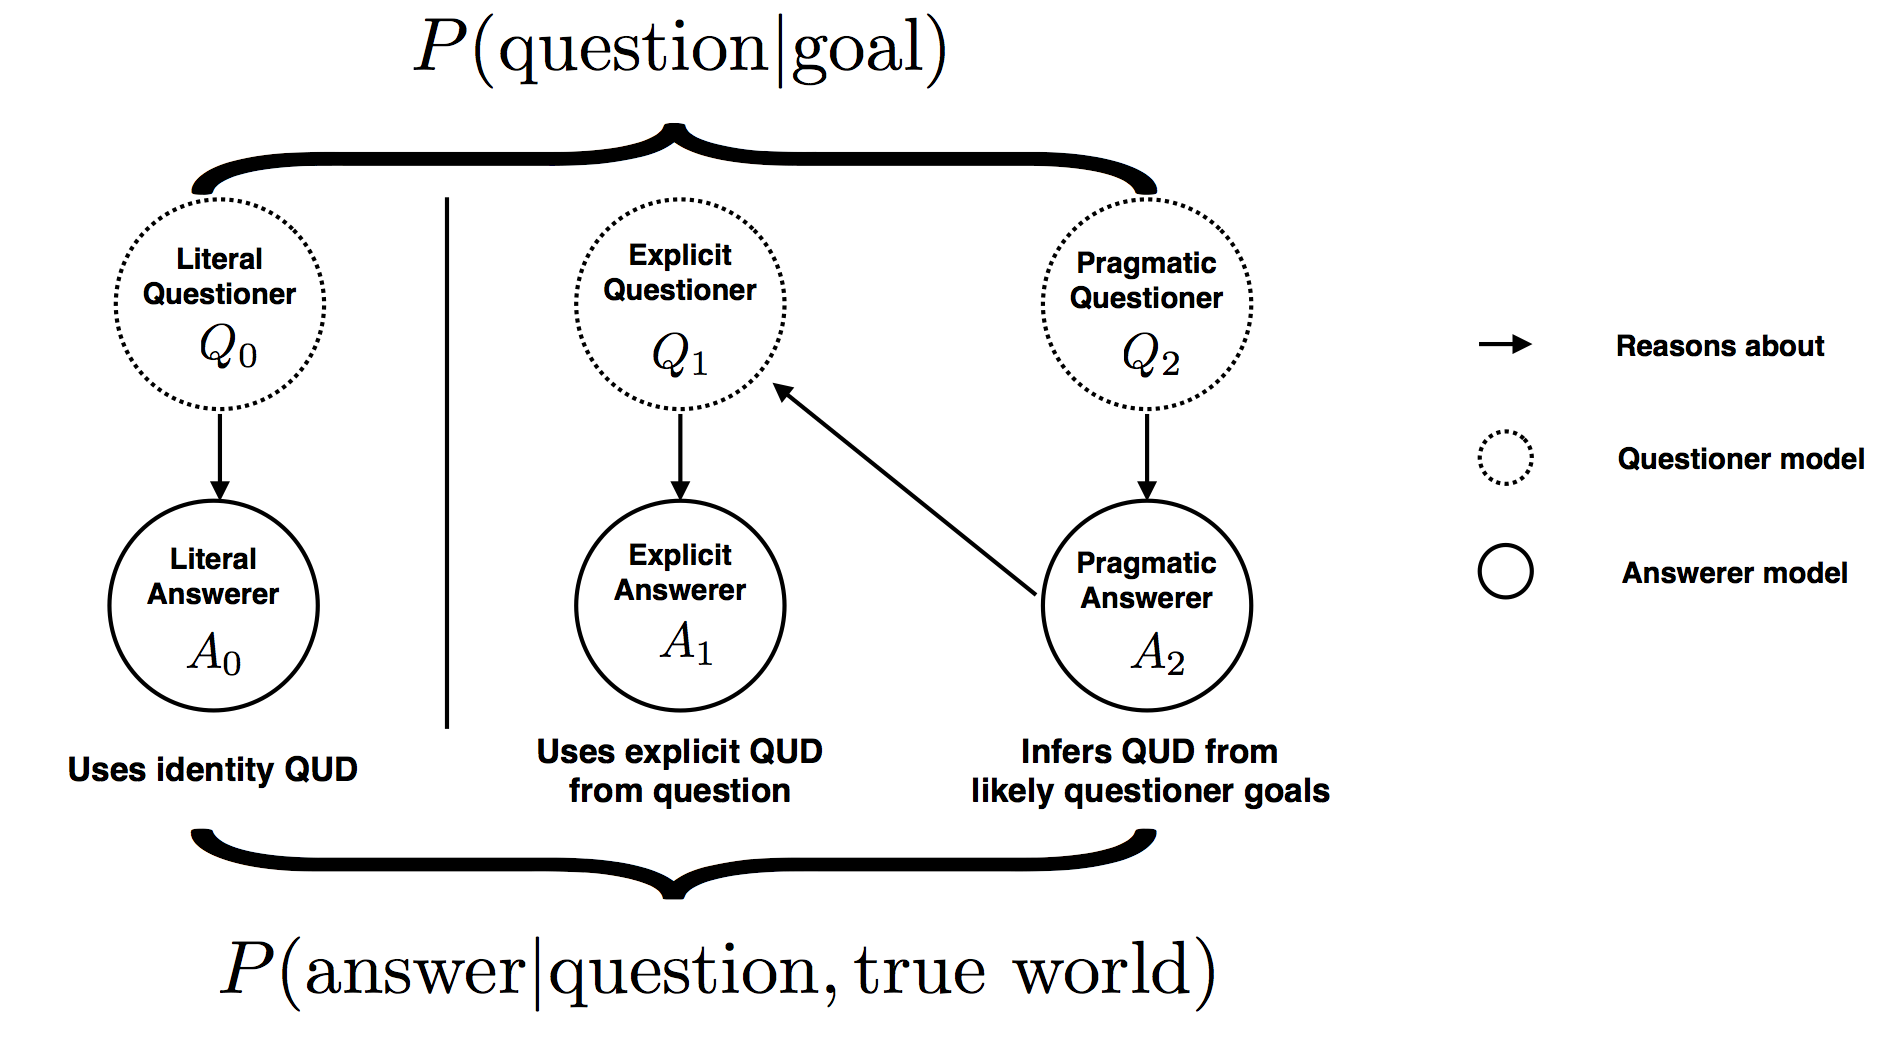
\includegraphics[scale = .5]{models.png}
\end{center}
\caption{Schematic of the questioner and answerer models we consider, showing their recursive relationships. Note that there are two possible ``base cases'' where the recursion can terminate: in a \emph{literal} answerer that ignores the question and simply attempts to be informative with respect to the world, and in an \emph{explicit} answerer that uses the semantics of the questions.}
\label{fig:models}
\end{figure*}

% HOW ARE THESE ADDRESSED IN RSA?
The listening problem and the speaking problem have been addressed separately in prior work within the Rational Speech Act (RSA) framework \cite{FrankGoodman12_PragmaticReasoningLanguageGames, GoodmanStuhlmuller13_KnowledgeImplicature, GoodmanFrank16_RSATiCS}, in which language understanding is formalized as recursive Bayesian inference. 
Pragmatic speaker agents choose utterances to maximize their partner's surprisal about the true state of the world -- a basic epistemic goal -- and pragmatic listener agents interpret utterances by inverting the speaker model. 
This basic framework has been used to account for a number of diverse pragmatic phenomena including 
scalar implicature \cite{GoodmanStuhlmuller13_KnowledgeImplicature}, %prosody \cite{BergenGoodman15_StrategicUseOfNoise},
%the acquisition of word meanings \cite{FrankGoodman14_InferringWordMeanings}, and
generic language \cite{TesslerGoodman16_Generics}, and
interpretation of context-sensitive adjectives like ``tall'' or ``cheap'' \cite{LassiterGoodman15_AdjectivalVagueness}.

% HOW IS GOAL-RELEVANCE FORMALIZED IN RSA?
RSA models have also recently been extended to incorporate the critical notion of \emph{goal-relevance} into the speaker's utility \cite{Roberts96_InformationStructureDiscourse, WilsonSperber12_MeaningRelevance}. 
Instead of attempting to be maximally informative about the \emph{full} state of the world, a goal-relevant speaker ignores irrelevant dimensions and only attempts to be informative about the relevant feature or summary statistic. 
RSA models with relevance have been used to capture non-literal language use like metaphor, irony, and hyperbole. 
In the case of hyperbole, for instance, a speaker who says ``It took a million years to get a table'' may be intending to be informative about the topic of their affective state (e.g. their frustration) rather than the exact time it took to get a table \cite{KaoWuBergenGoodman14_NonliteralNumberWords}.

% HOW IS OUR MODEL DIFFERENT FROM PAST MODELS (DIALOGUE!)
Although the social interplay between questioner and answerer may superficially resemble that of the \emph{speaker} and \emph{listener} agents in previous RSA models, the minimal form of dialogue introduced by a question-answer pair present fundamentally new challenges.
Here, we build upon these recent modeling advances in several ways. 

First, while the role of a speaker in prior models is limited to production, and the role of listener is limited to interpretation, question-answer dialogue requires unifying the listening problem and speaking problem in a single agent. 
Addressing this problem in a rational model requires derivating of the appropriate contingency between linguistic input and output.
Different kinds of input shift an agent's beliefs in different ways, motivating different kinds of responses. 

Second, the utilities considered in previous rational models of language use cannot straightforwardly capture the utility of a question, since questions -- as utterances -- don't provide direct information about the world to the listener.
While a declarative statement in our framework provides evidence about the true state of the world, as in previous models, we conjecture that a question provides evidence about the \emph{speaker's goals}. 
Rather than defining the meaning of a question in terms of its possible answers, as in traditional linguistic theories, we treat it as a \emph{signal} that the listener can use to update their beliefs about the goals of the question-asker. 
When it is the listener's turn to speak, they can then generate statements that better address the goal-relevant aspects of the world. 
In the next section, we review the basic RSA framework and explore several different proposals for how agents interpret and respond to questions within this framework.

%This is a first step toward chaining together more complex multi-utterance discourse phenomena.

% HOW IS OUR MODEL DIFFERENT FROM PAST MODELS (QUESTIONS!)
%\footnote{That is, the literal meaning of a question does not seem to be new information about the world, per se. Questions do, of course, end up conveying information about the speaker's knowledge, needs, and so on---it is this conveyed information that we attempt to derive below.}. 

 %This diverges from previous RSA models in that the value of a question depends on information gained by the speaker (rather than listener), and that this information comes later in the (very short) conversation. 

%The account of questioner and answerer behavior we propose in this section is a an effort to synthesize linguistic theories of question semantics with rich, quantitative cognitive models of language understanding. 
%We jointly model the questioner's choice of question and the and answerer's choice of answer through recursive social reasoning, allowing the answerer to \emph{infer} the questioner's private goal from observing the context and question utterance. 

%If the questioner determines what question to ask by reasoning about likely answers, we must specify what kind of answerer they are reasoning about. We explore three increasingly sophisticated kinds of answerers, which serve as possible internal models used by the questioner, yielding three increasingly sophisticated kinds of questioners; these three models serve also independently as models of actual answerers. 
%The simplest agent, the literal answerer, simply attempts to be maximally informative about the true state of the world, ignoring the question;   
%the explicit answerer assumes that the question has a context-independent meaning and attempts to be informative with respect to that meaning (without inferring the questioner's underlying interests);  
%the pragmatic answerer treats the question as a signal to the questioner's underlying goals, infers the most likely underlying interests of the questioner, and then informatively addresses those interests (see Figure \ref{fig:models})\footnote{In terms of \citeA{VanRooy03_QuestioningDecisionProblems}, the meaning function used in the explicit models corresponds to the first proposal of context-independent semantics, while our pragmatic models roughly correspond to the second.}. 
%The latter model uses an extension of RSA to reason about the topic of conversation, as proposed by \citeA{KaoWuBergenGoodman14_NonliteralNumberWords}; it goes beyond previous work by using the explicit question as a (potentially indirect) cue to this topic. 

\label{sec:model}

\subsection{Preliminaries}

Our mathematical formalization of dialogue begins with four primitive sets that agents take to be in common ground. For concreteness, we use the scenario from \citeA{Clark79_IndirectSpeechActs} as an example throughout: 
\begin{description}
\item[$\mathcal{W}$:] a set of true states of the world, such as the true price of a bottle of whiskey \{\$1, \$2, \dots, \$10\}. In principle, this may also include other features of the world, such as the current weather, the location of nearby caf\'es, or the kinds of payment that the store accepts.
\item[$\mathcal{G}$:] a set of possible underlying questioner goals, such as learning the actual price of the whiskey or learning whether or not one can afford to buy the whiskey at all. 
We formalize the key notion of an informational goal $g \in \mathcal{G}$ as a projection function $g: \mathcal{W} \rightarrow \widehat{\mathcal{W}}$ that maps a world state $w$ to a particular feature or set of features that the questioner cares about, which we denote $\widehat{w} = g(w)$; this is similar to the notion of a question-under-discussion \cite<QUD;>{Roberts96_InformationStructureDiscourse}. For example, the customer's goal of learning the actual price of the whiskey is given by the identity function $g_{=}(w) = w$, while the goal of learning whether it is affordable is given by 
$$g_{<}(w) = \left\{\begin{array}{rcl}
1 & & w < 5 \\
0 & & \textrm{otherwise}
\end{array}\right.$$
such that all worlds where the agent can afford the whiskey are mapped onto one state, and all other worlds are mapped onto a different state.
\item[$\mathcal{Q}$:] a set of possible question utterances , such as ``Does a fifth of Jim Beam cost more than \$5?'' or alternatives like ``Do you accept credit cards?'' We take the literal meaning \den{$q$} of a question to be of the same type as informational goals, such that a particular question utterance corresponds to a particular goal projection\footnote{This is equivalent to the more common partition semantics of \citeA{GroenendijkStokhof84_SemanticsOfQuestions}, as can be seen by considering the pre-image of such a question projection: $q^{-1}(\hat{w})$.}. For example, the literal meaning of the question ``Does a fifth of Jim Beam cost more than \$5?'' is a function that maps all worlds $w$ such that $w > \$5$ to one value and all other worlds to a different value. Note that the correspondence between questions and goals is not necessarily symmetric: while every question corresponds to a goal, we do not expect that every possible goal corresponds to a question utterance.
\item[$\mathcal{A}$:] a set of possible declarative utterances, such as ``It costs \$7.'' or ``Yes, it costs more than \$5.'' We take the literal meanings of these declarative utterances \den{$a$} to be truth-conditional: a map from world states to booleans. For instance, the utterance ``A fifth costs \$8.'' would be true in the world where $w = \$8$ and false otherwise. 
\end{description}
%QUDs are often used in formal linguistic models to capture \emph{relevance}: there are many informative sentences one can use to convey a full world state, but only a few of those are informative with respect to the current topic of discussion. \ndg{this comment about relevance seems out of place.}

\subsection{$A_0$: Informative Answerer}

We begin by considering the problem of how a dialogue agent ought to interpret and respond to a question utterance. The simplest baseline answerer, $A_0$, attempts to be informative about the state of the world without considering his partner's goals. In other words, $A_0$ is a rational speaker without any corresponding listener component to interpret and relevantly address its input. 

Formally, $A_0$ hears a question utterance $q \in \mathcal{Q}$ with private knowledge about the true world state $w \in \mathcal{W}$. He then uses a soft-max decision rule to choose an utterance $a \in \mathcal{A}$ proportional to the epistemic utility of that utterance to his communication partner: 
$$P_{A_0}(a | q, w) \propto \exp(\alpha U_{A_0}(a;w))$$ 
where $\alpha$ is a soft-max optimality parameter. 

We define the epistemic utility of the utterance using the information-theoretic measure of surprisal: the increase in an imagined interpreter $I$'s certainty about the true state of the world after hearing $a$: 
\begin{equation}
\label{eq:A0utility}
U_{A_0}(a;w) = \ln P_I(w|a)
\end{equation}

Critically, $A_0$ assumes that $I$ uses Bayesian inference to update their beliefs about worlds, conditioning on the literal meaning of the utterance $a$ being true:
$$P_I(w|a) \propto \delta_{\textrm{\den{a}}(w)} P(w)$$
where $\delta_{e}$ is the delta function returning 1 when $e$ evaluates to true and 0 otherwise, and $P(w)$ is a prior over true states of the world. 
%In other words, the interpreter constrains the prior on worlds to the subset of its support that is consistent with the given utterance, and $A_0$ attempts to (soft)-maximize the probability of the true world in this posterior. 

This formulation of $A_0$ is equivalent to the pragmatic speaker $S_1$ for declarative statements in previous RSA models \cite{GoodmanFrank16_RSATiCS}. It thus serves as a useful baseline model for several reasons: for one, it chooses utterances using the same basic utility as the more sophisticated models we consider, thus serving as a ``lesioned'' speaker to evaluate the necessity of the listener component. At the same time, it is a more charitable baseline than a purely random speaker: if asked about a fifth of Jim Beam knowing that it costs \$8, $A_0$ would prefer ``It costs \$8'' to ``It costs more than \$5'' or (falsely) ``It costs \$4'' simply because the former leads to an interpreter placing more probability on the true state of the world ($w = $ \$8).

%%%
%\footnote{For the purposes of this paper, we assume answers are always full sentences, corresponding to truth-functional propositions that can be evaluated in a given world. The interpreter described is the simplest required to model such answers. For fragments such as `yes' or `Bob,' which can be used to answer questions like `Is dinner at 7pm?' or `Who got the promotion?' we would require a more sophisticated interpreter that can compositionally expand the fragment into a valid proposition, using the question. This is a standard operation in formal semantic models, and an interesting target for future research, but is not necessary for the experiments we report.}

\subsection{$A_1$: Relevantly Informative Answerer}

While $A_0$ is informative, he is not particularly \emph{relevant}. When asked about the weather, he is just as likely to inform his partner about what he ate for breakfast as he is to say ``it's sunny.'' How do we incorporate relevance into the answerer's utility? 

Following \citeA{KaoWuBergenGoodman14_NonliteralNumberWords}, we formalize speaker relevance by means of a projection function. Instead of trying to increase the listener's certainty about the most fine-grained true world state, a relevant speaker only cares about the listener's certainty in a coarser space in which irrelevant features have been collapsed together. That coarser space is the image $\widehat{\mathcal{W}}$ of the goal-projection $g$.
%$$\widehat{P^g}(w') = \sum_{w\in\mathcal{W}} \delta_{w' = g(w)} P(w)$$ 
Thus, we modify the utility from Eq. \ref{eq:A0utility} to define a relevantly informative answerer $A_1$: 
\begin{equation}
U_{A_1}(a; g, w) = \ln \sum_{w' \in \mathcal{W}} K_g(w, w') P_I(w' | a)
\end{equation}
where $K_g(w,w')$ is a similarity function (or kernel) between worlds, given by the goal. For the discrete space of goals considered in the current work, we use the delta function $K_g(w,w') = \delta_{g(w)=g(w')}$ which combines the probabilities of all worlds that map to the same value in $\widehat{\mathcal{W}}$\footnote{Note that $g$-projection is a generic operation on any probability distribution $P(w|\,\cdot)$, which we denote: 
$$\widehat{P}^g(w|\, \cdot) = \E{P(w'|\, \cdot)}{K(w,w')}$$
%\todo[inline]{rdh: not 100\% satisfied with this notation}
}.

%$$
%\begin{array}{rcl}
%U(a; g, w) & = & \ln \widehat{P^g_I}(g(w)|a) \\
%                 & = & \ln \sum_{w'\in\mathcal{W}} \delta_{g(w) = g(w')} P_I(w' | a) \\
%                 & = & \ln \sum_{w'\in\mathcal{W}} K_g(w,w')P_I(w' | a)
%\end{array}
%$$
This modified utility suggests simply using the semantics of the question $q$ itself as the goal projection:
$$P_{A_1}(a|q,w) \propto \exp(\alpha U_{A_1}(a; q,w))$$
This implements the most common theory of answerers in dialogue: $A_1$ directly interprets a question as an epistemic goal, then informatively produces an utterance that reduces the questioner's uncertainty under that goal projection. 

$A_1$ may be sufficient for many simple, fact-based questions, like ``Who was the 16th president of the U.S.?'' given a rich enough semantic parser to supply the semantics of $q$ \cite{BerantChouFrostigLiang13_FreebaseQAPairs}. Still, the dazzling display of context-sensitivity and indirectness displayed in everyday communication suggests that deeper social reasoning may be at play. To explore more sophisticated answerers that reason about context and their partner's underlying goals, we must first address the problem of how a speaker chooses between questions.

\subsection{$Q_i$: Questioners}

If the utility of uttering a declarative statement is imparting information about the true state of the world, what is the utility of uttering a question? We begin by assuming that a questioner aims to \emph{learn information relevant to a private goal}.
%
In order to choose a question that results in useful information, the questioner reasons about how her dialogue partner would respond in different possible states of the world. She then selects a question that results in an answer that tends to reduce her own uncertainty about goal-relevant information.
%

% This is a divergence from previous RSA models, where agents choose utterances with the goal of imparting information about the state of the world.

More formally, a questioner agent takes a goal $g \in \mathcal{G}$ as input and returns a distribution over question utterances $q \in \mathcal{Q}$ by solving a simple planning problem involving two components: (1) which answers are likely to come back after asking this question, and (2) how much would be learned from each of those answers. Critically, in order to solve either of these parts, the questioner must have in mind an imagined answerer who hears her question and responds appropriately: thus, we have a family of questioners $Q_i$, each using the corresponding answerer $A_i$:
%
$$
\begin{array}{lcl}
P_{Q_i}(q|g)  & \propto & \exp\{\alpha U(q;g)\} \\
U(q;g) & = & \E{P(a|q)}{IG^g(a,q)} \\
	 & = & \sum_{w\in\mathcal{W}} P_{A_i}(a|q,w)P(w) IG^g(a,q)
\end{array}
$$
%

The expectation over likely answers $P(a|q)$ is computed by running an imagined answerer model forward, marginalizing over the possible worlds $w \in\mathcal{W}$ they might have knowledge of. The value of an answer depends on its \emph{information gain} $IG^g(a,q)$: the gap between the questioner's beliefs about the $g$-relevant state of the world before and after hearing an answer. Drawing again upon information theory, we formalize the notion of information gain using the Kullback-Leibler divergence between the $g$-projected prior distribution and posterior after hearing $a$.
%
$$
IG^g(a,q) = \KL{\widehat{P^g}(w|q, a)}{\widehat{P^g}(w)}\\
$$
%

In order to anticipate her posterior beliefs after hearing an answer, the questioner must again make use of an imagined answerer, but now imagining herself as a listener in the future and inverting that model to infer the true world the answerer was trying to communicate:
$$P(w|q,a) \propto P_{A_i}(a| q, w)P(w)$$

Note that $Q_0$, who plans their question by reasoning about the likely responses of $A_0$, does not prefer any utterance over any other, because they will all lead to the same distribution of (informative) answers. $Q_1$, on the other hand, expects $A_1$ to directly interpret her question as a goal and respond informatively and relevantly, thus allowing for some questions to be better than others. It therefore instantiates the same expected information gain measure of usefulness as proposed by current Optimal Experiment Design (OED) models of human inquiry \cite{coenen2018asking}. Critically, in contrast to \citeA{GroenendijkStokhof84_SemanticsOfQuestions} and \citeA{VanRooy03_QuestioningDecisionProblems}, the questioner's behavior is not governed fully by the semantics of the question she asks, but by what she actually expects her partner to say after hearing it. They may be the same when reasoning about the simple $A_1$ answerer, but we next turn to a more socially perspicacious answerer where they diverge.

\subsection{$A_2$: Goal-Sensitive Answerer}

%How should an answerer choose between answers to a question? What should a questioner assume about the answerer when choosing a question? We next describe three different answerer models; the questioner could assume any one of them, leading to three corresponding versions of the questioner model. From here on, we index the questioner and answerer models by $i$ to formulate different questioner models $Q_i$ which reason about different answerers $A_i$ (see Figure \ref{fig:models}).
%All answerers take a question $q \in \mathcal{Q}$ and a true world state $w^* \in \mathcal{W}$ as input and return a distribution over answers $a \in \mathcal{A}$.
%

%The \textbf{literal answerer} simply chooses answers by trading off prior answer probability (interpreted here as cost) and how well that answer conveys the true state of the world to an interpreter:
%%
%$$P_{A_0}(a | q,w^*) \propto e^{P_I(w^* | \,a) - C(a)} $$
%\ndg{isn't there a $\ln$?}
%%

% \todo[inline]{this is wrong (should prefer \emph{it costs 8})}
%For a fixed question, this is equivalent to the speaker in previous RSA models. They seek to be maximally informative about the state of the world, but do not adjust their response for different question utterances or contexts. This model is of interest primarily as a null model that is nonetheless more realistic than a random speaker. 
%

%\begin{table*}[h!]
%\centering
%\begin{tabular}{ p{5.15cm} | p{4cm} | p{7cm}}
%Case study &	Cue to goals	& Model variations \\
%\hline
%Clark (1979); Exp 4 &	prior verbal context	& likely goals depend on context \\
%\hline
%Groenendijk \& Stokhof (1984) & non-verbal features & multi-dimensional world representation, expanded space of answers \\
%\hline
%Gibbs Jr. \& Bryant (2008)  &	current world state &	expanded space of possible goals\\
%\hline
%Clark (1979); Exp 5 & choice of question & expanded space of question alternatives 
%\end{tabular}
%\\[1.5pt]
%\caption{Overview of the key features of the case studies we consider, and the modeling choices we make in each case. Note that while representations of sets $\mathcal{W}, \mathcal{Q}, \mathcal{A},$ and $\mathcal{G}$ adjust to capture the details of each scenario, the overall model framework is held constant.} 
%\end{table*}

Now that we have defined the utility of asking a question, we can construct our final pragmatic answerer: $A_2$. The speaker component of this answerer attempts to informatively and relevantly address the questioner's goal like $A_1$. The listener component, however, accounts for the generative process of an asker with an underlying goal rather than taking that goal to be identical to the literal meaning of the question. That is, $A_2$ assumes that the question was produced by a rational agent $Q_1$, who is trying to address a private goal $g \in \mathcal{G}$, and then attempts to be relevantly informative with respect to his posterior over \emph{underlying} goals $P(g|q)$ given the question:
\begin{equation}
U_{A_2}(a; q, w) = \sum_{g \in \mathcal{G}} P(g|q) \widehat{P^g_I}(w|\,a)
\end{equation}

%The \textbf{pragmatic answerer} also evaluates answers with respect to how well they address the questioner's goal, but doesn't take the question's explicit meaning at face value. Instead, the pragmatic answerer reasons about which underlying goals $g$ are likely given that a question $q$ was asked, and chooses answers that have high expected informativity:
%
Reasoning backwards from questions to goals is a simple Bayesian inversion of $Q_1$ using a prior on goals:
$$
P(g|q) \propto P_{Q_1}(q|g)P(g)
$$

By defining $A_2$ recursively in terms of $Q_1$, we implicitly give rise to an arbitrarily deep chain of nested reasoning where $A_{i}$ infers a posterior over underlying goals by inverting $Q_{i-1}$, and so on. This recursion terminates in the base case $A_1$, which uses the literal question semantics. For our purposes, however, we only consider models up to a depth of $i=2$, after which there are no qualitative changes in the model's behavior in the cases we examine\footnote{Recent systematic model exploration by \citeA{frank2017rational} suggests that recursive depth trades off with the soft-max optimality parameter $\alpha$. Because these two parameters are not generally identifiable, we fix the maximal level of recursion and achieve the behavior of higher levels of recursion by allowing $\alpha$ to vary.}. In particular, we are interested in $Q_2$, which can be interpreted as an agent who rationally selects a question not simply for its literal meaning but for the signal it provides about her underlying beliefs. This concludes our specification of the model space, giving a set of three answerers and three corresponding questioners that reason about them (see Fig. \ref{fig:models})\footnote{We have implemented these models in WebPPL, a probabilistic programming language \cite{GoodmanStuhlmuller14_DIPPL}. Reproducible experimental materials as well as code for all reported analyses and model simulations is available at \url{https://github.com/hawkrobe/Q\_and\_A}}.
 

%For all of the questioner and answerer models, we can vary how strongly optimizing they are---that is, to what extent they are sampling from the distributions defined above, and to what extent they deterministically choose the most likely element. For any such distribution over utterances, we introduce an optimality parameter $\alpha$ and transform it by $ P'(x) \propto P(x)^{\alpha} $. Furthermore, we have set the answer prior in all answerer models such that outright false responses are excluded. The answerer models naturally assign very low, but non-zero probability to these options (because they are minimally informative). However, we set them to zero probability for the sake of simplicity in reporting and visualizing predictions.
%



\section{Case studies in answerer sensitivity}

In this section, we illustrate our \emph{answerer} models through several classic goal-sensitivity effects reported by \citeA{Clark79_IndirectSpeechActs}. These case studies center around three empirical observations about the factors determining answerer behavior in dialogue. First, and most obviously, answers should be sensitive to the surface form of the question utterance: ``What time do you close tonight?'' should elicit a different distribution of responses than ``What is the price of a fifth of Jim Beam?''. Second, answers should be sensitive to context: the \emph{same} question utterance elicits different responses across contexts where different goals are more or less likely. Third, and most subtly, answers should be sensitive to the cue provided by the question utterance itself toward the questioner's underlying goals\footnote{These examples are implemented and runnable at \url{forestdb.org/models/questions-answers.html}}.


% We proceed to demonstrate the way our model addresses four classic examples of question and answer pragmatics from the psycholinguistics literature. There has been little use of questioner behavior as a dependent variable in previous literature, hence our examples explore the sensitivity of the answerer to plausible goals of the questioner. 
%These examples do not serve as a strong test of our model's predictions, because we will have to make post-hoc assumptions about prior distributions or goal spaces in each study.

%Yet it is important to show that our framework can accommodate these results.
%We see two additional benefits to re-formulating explanations from the original studies within our modeling framework: (1) the case studies are instructive as examples of how different components of the model interact to generate results and (2) by placing all four studies in a common framework, we more clearly see their commonalities and differences. 

%\ndg{i feel like this section gets pretty quickly lost in the weeds.... maybe we can reorganize it around the effects or model components explored? and move some of the details and conceptually redundant pieces to appendices?}

% \begin{figure*}[t!]
%\begin{center}
%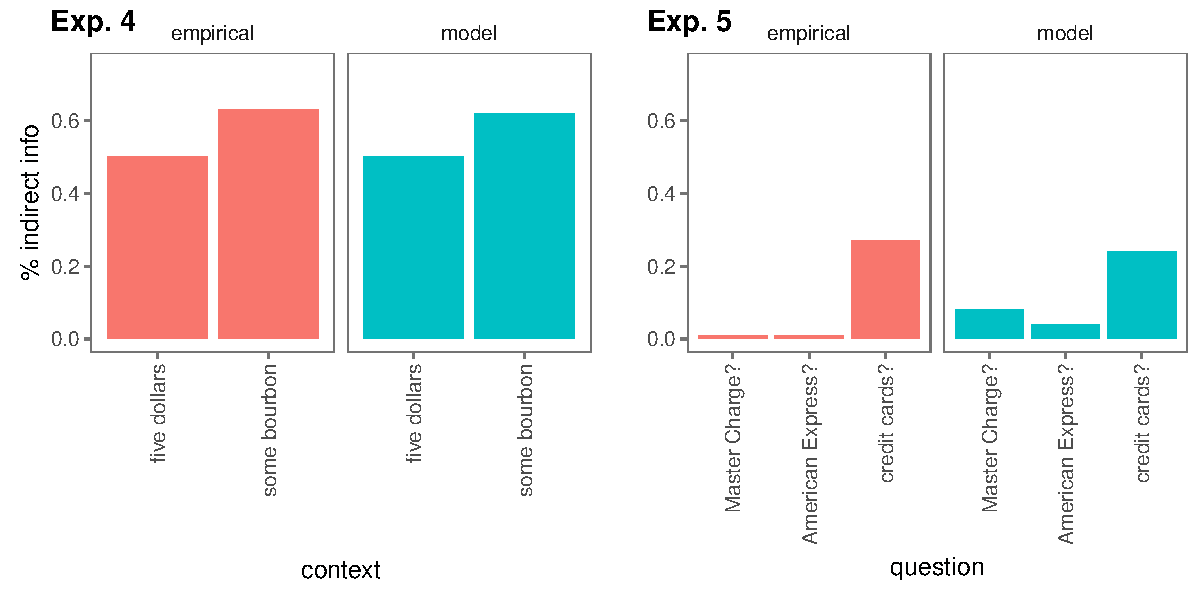
\includegraphics[scale = .6]{clarkCaseStudies.pdf}
%\end{center}
%\vspace{-.25cm}
%\caption{Comparison of questioner goal posteriors that the pragmatic answerer model infers after hearing two different question utterances in Clark (1979), Experiment 5.}
%\label{fig:clarkResults}
%\end{figure*}

%\begin{table*}[t]
%\centering
%\begin{tabular}{ p{3cm} | r | r ||||||  r | r }
%& \multicolumn{2}{c||||||}{Empirical} & \multicolumn{2}{c}{Model} \\
%\hline
%&           \% literal &   \%  info &           \% literal &   \%  info    \\
%\hline
%``Some bourbon'' &   0.37 & 0.63 &  0.38 & 0.62 \\
%\hline
%``Five dollars''     & 0.50 & 0.50 & 0.50 & 0.50 \\
%\specialrule{2.5pt}{1pt}{1pt}
%``Master Charge cards?'' &   1.00 & 0.00 &  0.92 & 0.08 \\
%\hline
%``American Express cards?''     & 1.00 & 0.00 & 0.96 & 0.04 \\
%\hline
%``Credit cards?''     & 0.73 & 0.27 & 0.76 & 0.24 \\
%\end{tabular}
%\\[1.5pt]
%\caption{Comparison of model predictions and data from Clark (1979). Shows the proportion of responses to the question ``Does a fifth of Jim Beam cost more than \$5?'' when paired with two contexts: ``I want to buy some bourbon'' (``Some bourbon'') and ``I've got \$5 to spend'' (``Five dollars''). } 
%\label{table:clark79exp4}
%\end{table*}

\subsection{Sensitivity to question utterance}

The minimal requirement for any answerer model is that it behaves differently in response to different questions. This can also be considered a special case of the minimal requirement for a dialogue agent: that their behavior at time $t$ is in some way dependent on their partner's at $t-1$. %We briefly illustrate this phenomenon in our model using two example sentences lightly adapted from \citeA{Clark79_IndirectSpeechActs}.
Consider the problem faced by a liquor store cashier answering one of the phone calls reported by \citeA{Clark79_IndirectSpeechActs}: they may be asked one of two questions: $q_t$ (``What time do you close tonight?'') and $q_p$ (``What is the price of a fifth of Jim Beam?''). How do our answerer models respond to each of these questions?

To model this situation, we take a world $w \in \mathcal{W}$ to be a tuple containing the closing time and the price of Jim Beam at the store in question. Thus, $\mathcal{W}$ is the set of all possible tuples $w = (t, p)$, where $t$ is a time in the (simplified) set $\{9\textrm{pm},10\textrm{pm}\}$ and $p$ is a price in $\{\$4, \$5, \$6\}$. Similarly, we consider a simplified set of answers $\mathcal{A}$: an answerer may either state a time $a_{t_i}$ (``We close at 9:00.'') or the price of Jim Beam $a_{p_i}$  (``A fifth costs \$5.''). These utterances evaluate to true in a particular world $w$ if and only the stated dimension has the stated level.

Our informative answerer $A_0$ does \emph{not} reply differently to the two questions. In either case, he slightly prefers to inform the questioner about the price using $a_{p_i}$ because he reasons that a literal interpreter $I$, after hearing such an utterance, would be left with uncertainty over only two possible worlds (where the closing time is either 9:00 or 10:00) rather than the three possible worlds consistent with an utterance stating the true time (where the price is either \$4, \$5, or \$6).

Both $A_1$ and $A_2$, on the other hand, appropriately give different answers to the two questions, though for different reasons. $A_1$ gives different answers because the two questions simply have different literal meanings: $q_t$ projects a world $w_i = (t_i, p_i)$ to its first element:$$q_t(w_i) = t_i$$ whereas $q_p$ projects $w_i$ to its second element $p_i$. In this example, because we take the space of goals $\mathcal{G}$ to contain these same two projections, $A_2$ makes essentially the same inference. He reasons it's more likely, via Bayes' Rule, that a questioner agent $Q_1$ who chose to ask $q_t$ would have the goal of learning the closing time than the price, and updates his beliefs accordingly.

These answerers then choose an utterance that \emph{relevantly} addresses the goal they inferred. $a_{p_i}$, for instance, would leave the questioner with perfect information about $p_i$ but gives no information at all about $t_i$. Thus, it would be a preferred response to $q_p$ and a dispreferred response to $q_t$. This shows the desired sensitivity to question.

\subsection{Sensitivity to context}

Next, we show how our models can provide different---sometimes over- or under-informative---answers to the same explicit question, depending on context. For this illustration, we consider the results of Experiment 4 from \citeA{Clark79_IndirectSpeechActs}. Recall that liquor merchants were more likely to give over-informative answers (specifying exact price) to the question ``Does a fifth of Jim Beam cost more than \$5?'' in the uninformative context (``I want to buy some bourbon'') than in the five dollar context (``I've got \$5 to spend''). Which of our answerer models, if any, shows a similar sensitivity to context?

Our space of possible worlds consists of possible prices for the whiskey: $\mathcal{W} = \{\$1, \dots, \$10\}$. We consider two possible goals: $g_=$, learning the actual price of whiskey,  and $g_>$, learning whether or not the agent can afford to buy the whiskey at all (i.e. whether the price is greater or less than the amount the agent has in their pocket). The set of answers $\mathcal{A}$ includes exact prices $a~\in~\{\$1, \dots, \$10\}$ as well as ``yes'' and ``no.'' We use an answer prior that assigns equal probability to picking the category of ``yes/no'' answers and of ``price'' answers, then uniformly draws from the possible responses within each category. 

%Because the question was fixed in the experiment, the question space $\mathcal{Q}$ simply consists of the single question $q = $``Does a fifth of Jim Beam cost more than \$5?''\footnote{Note that because there are no alternatives for the ``pragmatic answerer'' to consider, they are not strictly engaging in Gricean reasoning; obvious alternatives like ``How much does Jim Beam cost?'' do not significantly change the model behavior in this case, but we omit them to isolate the effect of the QUD prior in this example.}  

We model the context sentence as a statement which the answerer must interpret before interpreting the question; we assume that it has the effect of shifting the answerer's beliefs about likely questioner goals $P(g)$ (presumably by shifting beliefs about how much money the questioner has to spend). When the context is ``I'd like to buy some whiskey,'' we assume that the the two goals are equally likely: $P(g_= | c) = P(g_> | c)$. When it is ``I only have \$5 to spend,'' we assume that it is more strongly in favor the agent learning whether or not they can afford it: $P(g_> | c)~=~.99$. 

$A_0$ is unable to show sensitivity to context for the same reason that he did not show sensitivity to the question utterance: he does not adjust his beliefs on the basis of what he hears. Thus, he always prefers to say the exact price (e.g. ``The whiskey costs \$6'') because it leaves less uncertainty about the true state of the world.

Because $A_1$ simply uses the literal meaning of the question, which is context-independent and not tied to the questioner's goals, he does \emph{not} give different responses in the two contexts. In either case, he is ambivalent between giving a yes/no answer and an exact answer because they are equally successful at distinguishing whether the true price is greater than or less than \$5. 

Finally, we see that $A_2$ is context-dependent in the same way as \citeA{Clark79_IndirectSpeechActs} observed. When the question is prefaced with ``I only have \$5 to spend,'' which shifts the answerer's beliefs about goals strongly toward $g_>$ (equivalent to the literal meaning of the question), then $A_2$ is equally likely to give both answers for the same reason as $A_1$ above. However, when the question is prefaced with ``I'd like to buy some whiskey,'' which leaves in place the answerer's uniform prior over goals, then the \emph{exact price} answer is favored more strongly. This answer is much more informative in the case when the questioner's goal is to know the exact price, and no worse in the other case. The expected value of the non-literal answer is thus higher, and the answerer responds proportionally. 
%The output of $A_2$ is shown in Fig. \ref{fig:clarkResults}, compared with empirical results from \citeA{Clark79_IndirectSpeechActs}\footnote{The responses in \citeA{Clark79_IndirectSpeechActs} were tallied in three categories: literal answer only $(n_l)$, information only $(n_i)$, or both literal answer \emph{and} information $(n_b)$. For the purposes of this case study, we are only interested in the ratio of literal answers to information answers: $p_l = n_l/(n_l+n_i)$ and $p_i = n_i/(n_l+n_i)$.}  
% This asymmetry arises in our model due to the fact that an exact price is much more highly informative than a literal response with respect to the ``exact price'' goal $g_=$, and if there is uncertainty over which goal is in fact the case, it is worth erring on the side of over-informativeness. This matches the empirical trend, which also favored the exact price answer (at probability $0.57$) over the literal answer (at probability $0.41$).

%This arises because both responses are equally informative with respect to learning whether or not the agent can afford the whiskey, $g_>$, so the response likelihoods fall back to the answer prior. This also matches the empirical trend, where the exact price and literal answer were equally likely.

%Note that the literal and explicit answerers do not take into account the questioner's underlying goals and therefore cannot reason about the way contextual factors may be informative about these goals. Hence, they do not make different predictions in the two contexts. The literal model predicts that the answerer is equally likely to say the true Boolean answer and the true numerical answer, and the explicit model predicts that the answerer will always give the true Boolean answer, since it is the explicit question being asked. This suggests that our pragmatic \emph{answerer} is consistent with human behavior in psychologically interesting situations, passing a first, qualitative, test. 

%\begin{table*}[t!]
%\centering
%\begin{tabular}{ p{5cm} | r | r ||||||  r | r }
%& \multicolumn{2}{c||||||}{Empirical} & \multicolumn{2}{c}{Model} \\
%\hline
%&           \% literal &   \%  info &           \% literal &   \%  info    \\
%\hline
%\end{tabular}
%\\[1.5pt]
%\caption{Comparison of model predictions and data from Clark (1979), Experiment 5. Shows the proportion of literal and over-informative responses restauranteurs gave to each of three different questions from a customer inquiring about credit cards.} 
%\label{table:clark79exp5}
%\end{table*}

\begin{figure*}[t]
\begin{center}
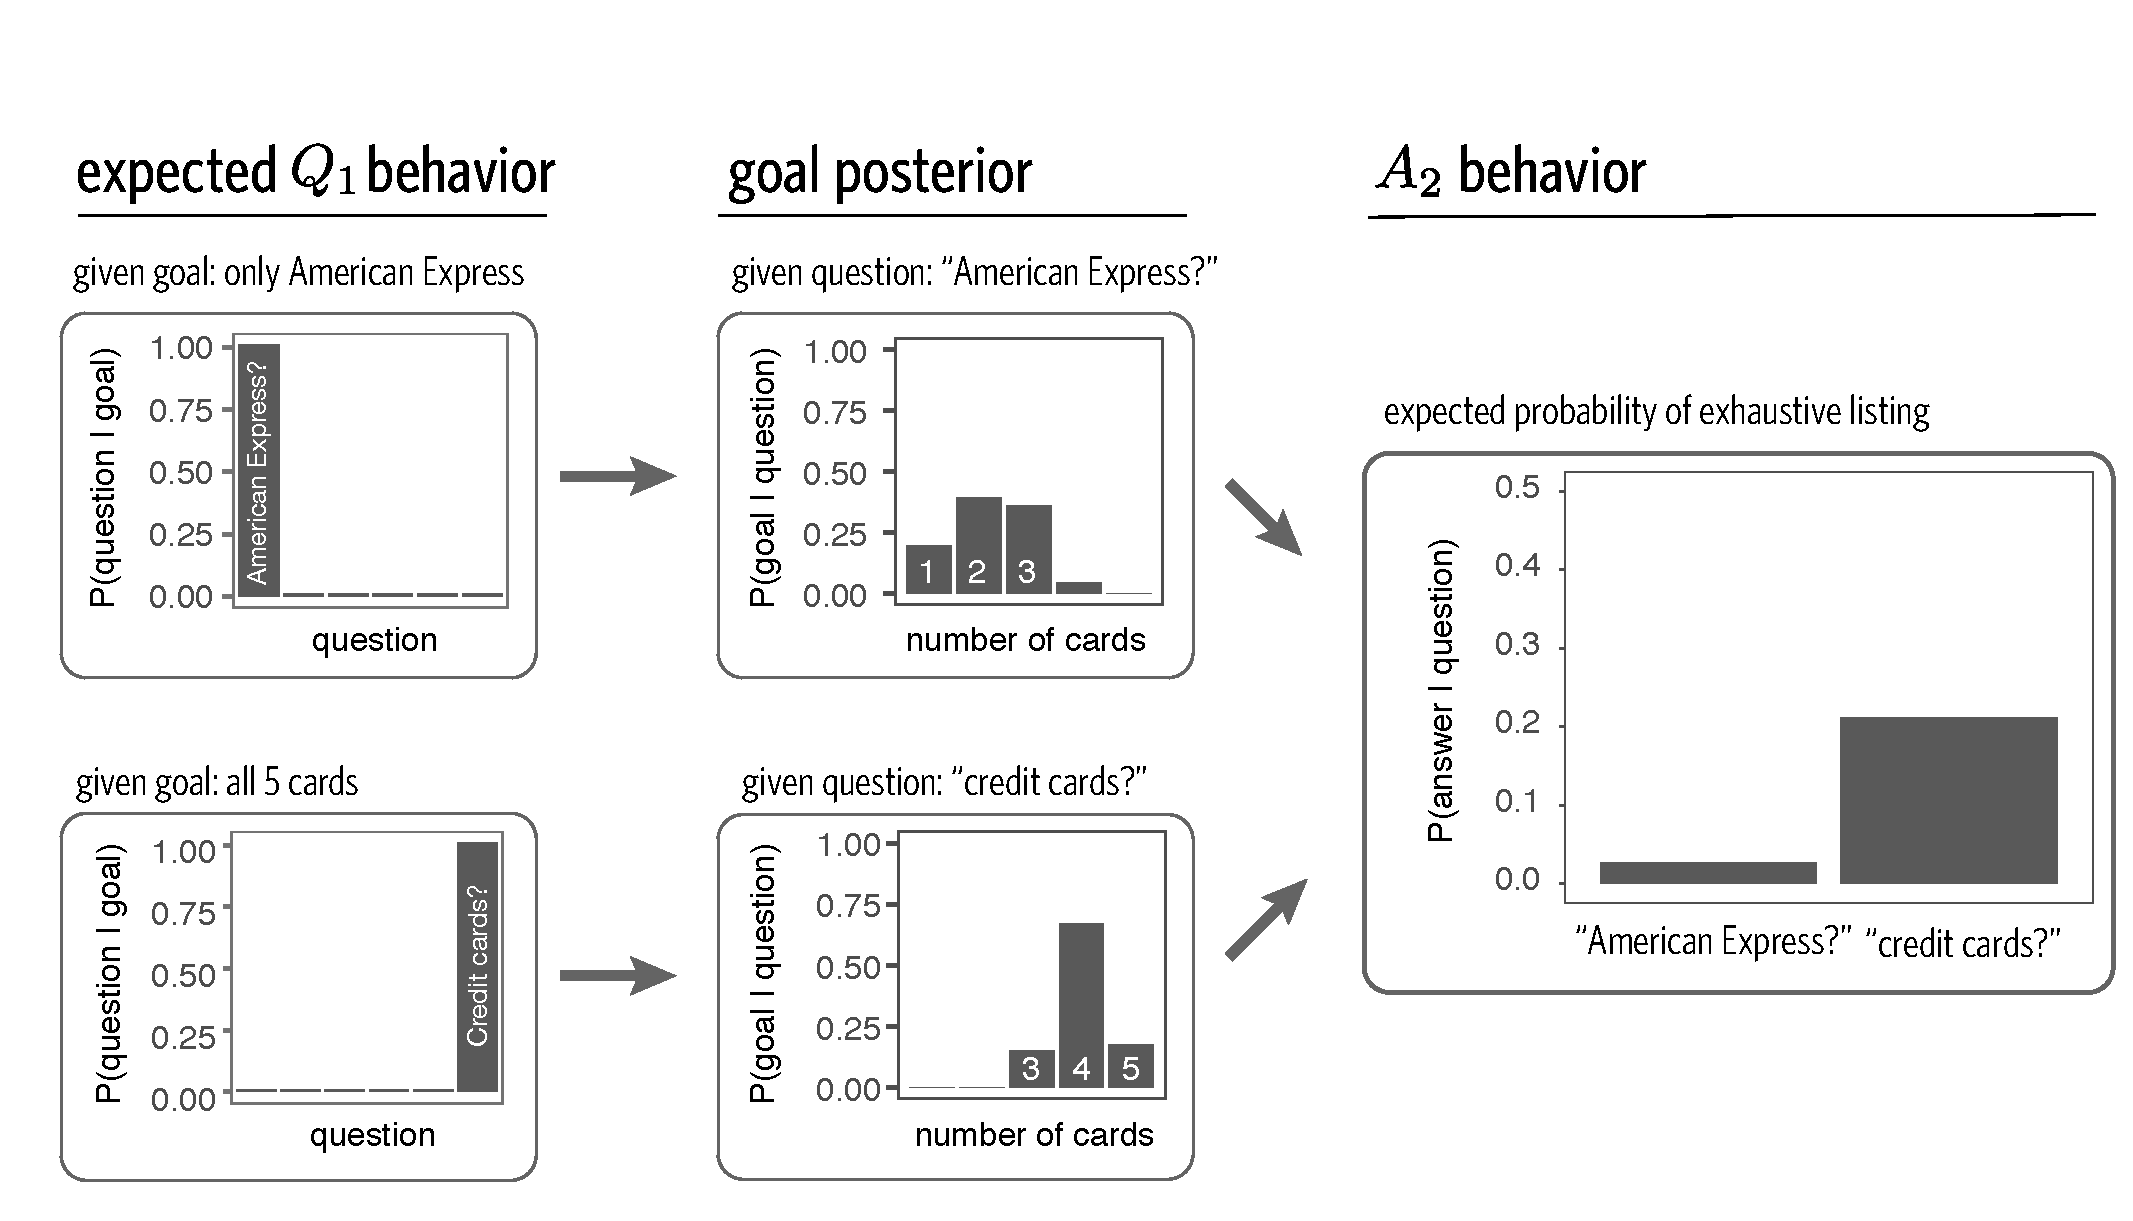
\includegraphics[scale=.5]{simulations/clarkExampleFig}
\end{center}
\vspace{-2cm}
\caption{Illustration of how $A_2$ uses the questioner's utterance as a cue to their underlying goal and responds relevantly, thus producing the sensitivity reported by Clark (1979). We set the optimality parameter $\alpha = 100$ to make the effect clearer; the middle column is the marginal posterior projected to the number of cards in the goal.}
\label{fig:clarkExample}
\end{figure*}

\subsection{Sensitivity to relationship between goal and question utterance}

% Our final scenario demonstrates the role of the questioner component in our pragmatic answerer model. Because the question space in the previous computational experiments only contained one element for simplicity, the pragmatic answerers' inferences were entirely based on the context and the QUD prior. One of the most interesting and novel predictions of the RSA model, however, is that the questioner's choice of utterance itself should guide a pragmatic answerer's inferences about likely underlying goals. The choice to ask one question instead of another provides information about the questioner's goal. While there are few previous experimental results using questioner behavior as the \emph{dependent variable}, there is some work manipulating the question asked as an \emph{independent variable} and testing how it affects answers.

The subtlest effects of answerer sensitivity go beyond the overt question utterance and context alone; given the same context, answerers may respond to one question according to its literal meaning but another using more indirect or overinformative statements. One of the key predictions of  $A_2$ is that these effects are due to different inferences about the questioner's \emph{underlying goals} on the basis of the questioner's choice of utterance itself. 

For our final case study, we consider Experiment 5 from \citeA{Clark79_IndirectSpeechActs}, which called restaurants and asked one of four yes/no questions about which \emph{credit cards} the restaurant accepted. We focus on three\footnote{
The fourth question was ``Do you accept any kinds of credit cards?'' We view Clark's results for this question as an example of M-implicature: by using a more costly utterance with the same literal meaning as question (3), the meaning becomes marked. Rational speech act models capture M-implicature by introducing \emph{lexical uncertainty} \cite{BergenGoodmanLevy12_Alternatives}, where both speaker and listener begin their inference with uncertainty over the literal meaning of utterances. % By jointly reasoning about an utterance's meaning and the world state the speaker is trying to convey, more costly utterances are mapped to meanings with lower prior probability, allowing a pragmatic inference that ``Do you accept any kinds of credit cards?'' most likely means something like ``What kinds of credit card do you accept?'' 
Because this is the only example of M-implicature that arises in this paper, and this is not the critical result from the experiment, we exclude it from our discussion.%believe that a presentation of the full lexical uncertainty model would be unnecessary and confusing to the reader.
}:
%%%
\begin{enumerate}
\item ``Do you accept Master Charge cards?'' 
\item ``Do you accept American Express cards?''
\item ``Do you accept credit cards?'' 
\end{enumerate}
%He analyzed the likelihood that the respondent gave a literal yes/no answer, compared to the likelihood of giving the exhaustive list of exactly which cards were accepted.  
\citeA{Clark79_IndirectSpeechActs} found that (1) and (2) were nearly always answered literally, with a `yes' or `no', while (3) was significantly more likely to be answered with full information. Which, if any, of our answerer models show this pattern of responses? % (see Table \ref{table:clark79exp5}). 
%As in the first case study above, we are only interested in the ratio of literal answers vs. over-informative answers $p_l = n_l/(n_l + n_i)$ and $p_i = n_i/(n_l + n_i)$, not in responses including both. 

We formalize the scenario as follows. The set of possible worlds $\mathcal{W}$ is given by the power set $\mathcal{P}(\mathcal{C})$, where $\mathcal{C} = \{$Visa, Master Card, American Express, Diner's Club, and Carte Blanche$\}$, the set of five possible credit cards. %This power set contains all $2^5 = 32$ subsets of cards that the restaurant might accept. 
The prior distribution over worlds, $P(w)$, can in principle take into account the empirical likelihoods of restaurants accepting different cards, but we treat them as uniform to make the dynamics of our simulations clearer. % Clark reports these likelihoods to be 72, 71, 38, 12, and 10\% for Visa, Master Card, American Express, Diner's Club, and Carte Blanche, respectively. 

The question space $\mathcal{Q}$ contains the five basic questions (``Do you accept $c$?" with $c \in \mathcal{C}$ one of the five cards) in addition to ``Do you accept credit cards?'' For the literal semantics of the five basic questions, indexed by $c$, we use the function $q_c(w) = \delta_{c \in w}$, which projects worlds to a boolean corresponding to whether they accept card $c$ or not.
%partitions the space of possible worlds into two cells: one  in which card $c$ is accepted and another in which it is not accepted. 
The latter question $q_{any}(w)  = \delta_{|w| > 0}$ projects to a boolean corresponding to whether any cards are accepted at all. %The prior distribution $P(q)$ over these questions is proportional to question length, which happens to be uniform.

The answer space $\mathcal{A}$ includes lists of cards (e.g. ``the cards we accept are Visa and MasterCard''), which are interpreted exhaustively, and  `yes' and `no.' We take the denotations of these polar responses to depend on the literal meaning of the previous question: $a_{\text{yes}}(w;q) = \delta_{\textrm{\den{q}}(w)}$ and $a_{\text{no}}(w;q) = \delta_{\neg \textrm{\den{q}}(w)}$.
 %Thus, the restauranteur could respond to the question ``Do you accept Master Charge cards?" by saying ``Yes'' or by saying something like ``We accept Visa and Diner's Club." 
%As in our early case study of Clark's (1979) whiskey experiment, we assign prior probability $p = 0.5$ to ``yes''/``no'' type responses, and prior probability $p = 0.5$ to card type responses, with uniform distributions within each category. 

Finally, all goal projections $g \in \mathcal{G}$ correspond to solving a simple problem: finding out whether the restaurant accepts at least one of a set of cards of interest (i.e. ``does the restaurant take any card in my wallet?''). This family of goals is parametrized by $\mathcal{C}_q \in \mathcal{W}$, the set of cards that the questioner is actually interested in: 
$g_{\mathcal{C}_q}(w) = \delta_{|\mathcal{C}_q \cap w | > 0}$.
%The prior $P(g)$ over goals is the same that governs the world prior. 
%\footnote{This corresponds to an assumption that restaurants accept cards proportional to the percentage of people being interested in those cards. This assumption was suggested by Clark (1979), but not used in his informal analysis).}. 
%Formally, for the goal $g_{\mathcal{C}_q}$, we define a projection to a boolean corresponding to whether the restaurant accepts at least one card in $\mathcal{C}_q$:
%$g_{\mathcal{C}_q}(w) = \delta_{|\mathcal{C}_q \cap w | > 0}$.

%For each possible question in the experiment, we tested the likelihood of our pragmatic answerer responding with a literal ``yes''/``no'' vs. an exhaustive list of accepted cards, marginalizing over all possible world states. For quantitative fit, we tuned a single rationality parameter $\alpha$, shared by all model components. For the results presented in Table \ref{table:clark79exp5}, we found the best quantitative fit when $\alpha \rightarrow \infty$. We use $\alpha = 10000$, since the predictions stabilize above this value. Recall that a high value of $\alpha$ corresponds to an agent that maximizes with respect to their probability distribution (i.e. always picks the utterance with highest probability, which is technically optimal)\footnote{Note that while we use deterministic QUDs for all scenarios in this paper, our implementation of the model in a probabilistic programming language makes it just as easy to use \emph{probabilistic} projections: mappings that partition the world space in different ways with different probabilities. If we instead use a family of goals $\mathcal{G}$ that samples uniformly from the cards of interest and project to 1 on worlds that contain \emph{the sampled card}, then we achieve the same results with a much lower $\alpha$. Probabilistic QUDs are currently non-standard in the semantics literature, and it will be interesting in future work to test the extent to which they provide a better pragmatic model}. 

% \begin{figure*}[t!]
%\begin{center}
%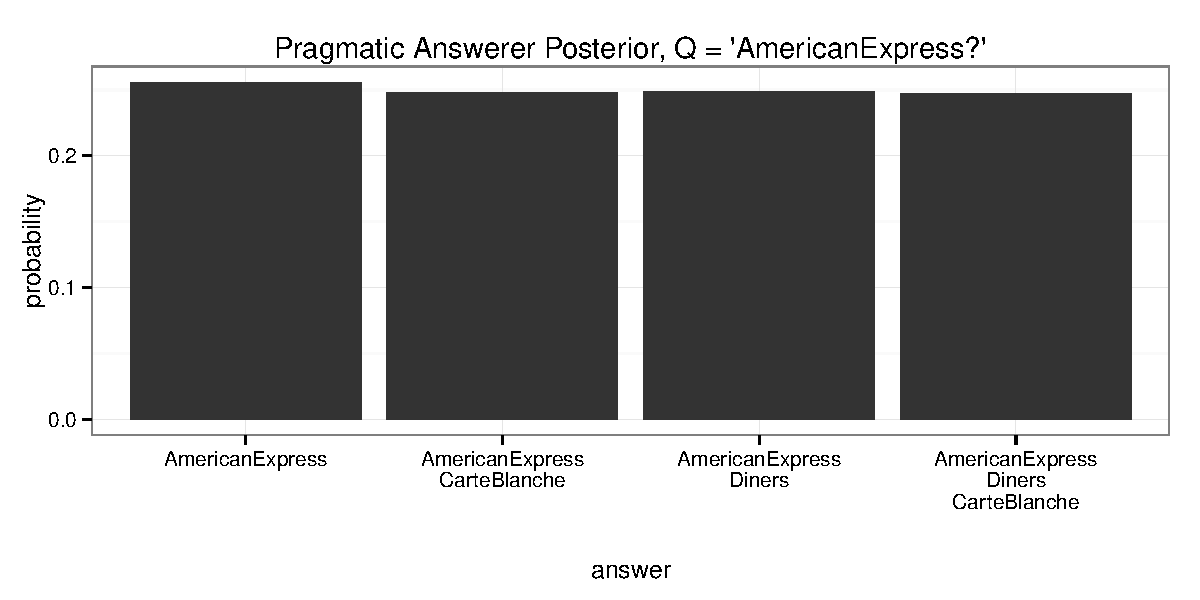
\includegraphics[scale = .6]{americanExpressPosterior.pdf}
%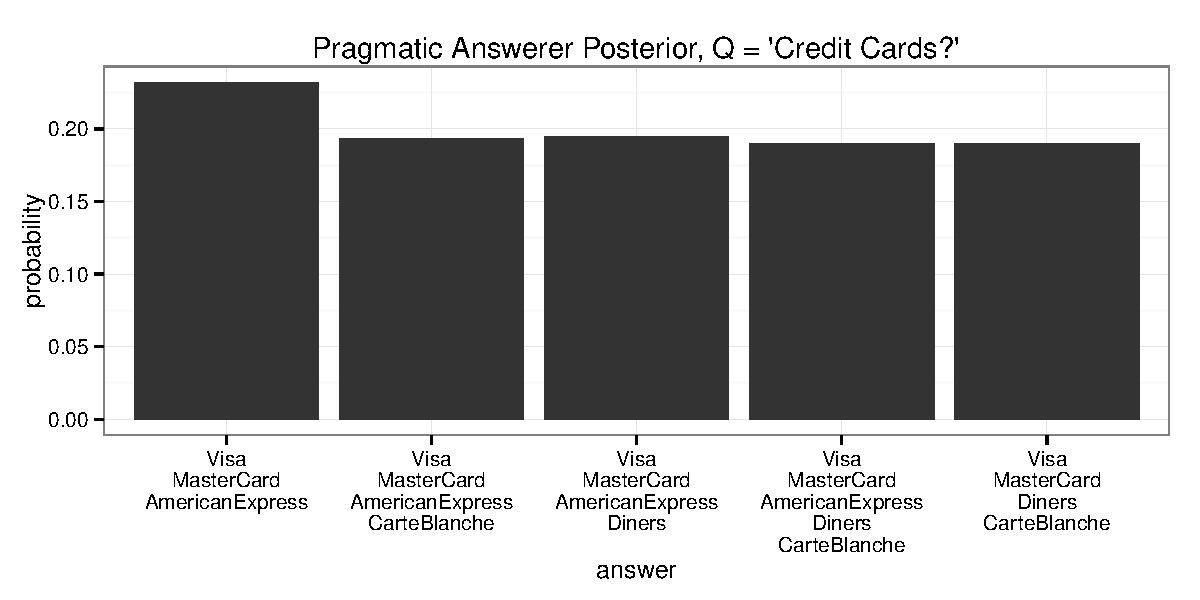
\includegraphics[scale = .6]{creditCardsPosterior.pdf}
%\end{center}
%\vspace{-.25cm}
%\caption{Comparison of questioner goal posteriors that the pragmatic answerer model infers after hearing two different question utterances in Clark (1979), Experiment 5. 
%\todo[inline]{There has to be a better way of presenting this result\dots}
%}
%\label{fig:clarkExperiment5posteriors}
%\end{figure*}

Because $A_0$ does not consider the question meaning, ``yes'' and ``no'' are not well-defined: the true list of cards is the most informative answer to any question, as it provides the exact identity of the true world. $A_1$, on the other hand, gives either a literal yes/no answer or indirect answer in proportion to their prior probability, regardless of which question is asked. Both answers provide complete information under the question projection.

By reasoning about the questioner's underlying goals, $A_2$ displays the pattern that \citeA{Clark79_IndirectSpeechActs} observed: a higher probability of giving a literal yes/no response to ``MasterCard?'' and ''American Express?'' than to "Credit cards?''. To understand \emph{why} $A_2$ behaves this way, we walk through the chain of pragmatic reasoning (Fig. \ref{fig:clarkExample}).

The key observation lies in the evidence provided by the question about the questioner's likely goal: $P(g | q) \propto P_{Q_1}(q|g)P(g)$. Consider two cases, beginning with the questioner's perspective  (right-most column of Fig. \ref{fig:clarkExample}). First, suppose $Q_1$ is only interested in an American Express card (goal $g_{\{AmEx\}}$). Any answer $A_1$ gives to $q_{AmEx}$ (the question ``American Express?'') would fully resolve her goal. ``Yes'' would yield certainty in accepting it and ``no'' in not accepting it. On the other hand, some answers to $q_{any}$ (``Credit cards?'') would not be resolving: if $A_1$ responded ``yes'', there would still be substantial uncertainty over whether the shop takes American Express in particular (for example, $A_1$ could informatively say ``yes'' if they only accepted Visa). A questioner with goal $g_{\{AmEx\}}$  is thus more likely to ask $q_{AmEx}$


%We find that when the questioner asks ``Do you accept MasterCard?'', the pragmatic answerer gives a literal ``yes''/``no'' answer with probability $p = 0.92$ (compared to $p=1.00$ empirically). Similarly, when the questioner asks ``Do you accept American Express?'', the pragmatic answerer gives a literal answer with probability $p = 0.96$ (also compared to $p=1.00$ empirically). The small difference between these predicted response probabilities comes from the relative likelihoods of the different cards in the true world. However, when the questioner asks ``Do you accept credit cards?'', the probability of a literal response drops to $p = 0.76$ (compared to $p=0.73$ empirically). Our model output therefore provides a good fit to the original experiment data, both qualitatively and quantitatively.

%\todo[inline]{integrate this paragraph}
%Under the literal semantics of questions that $Q_1$ is assumed to be using, a negative answer to a more specific question (e.g. finding out that the store does not take MasterCard) would leave $Q_1$ with uncertainty about whether any of her other cards would be accepted. Meanwhile, both positive and negative answers to ``Credit cards?''  would be quite informative: a negative answer would leave her certain about  Knowing whether the shop takes \emph{any} cards (as opposed to no cards) is more informative than knowing whether or not they take a specific one. 


Now, suppose instead that $Q_1$ has a long list of cards (say, all five: $g_{all}$). Then getting a yes/no for any one card would fail to address her goals: if she asked $q_{AmEx}$ and got a ``no'', she is still uncertain whether another card on her list would be accepted. On the other hand, $q_{any}$ is expected to be highly informative under $A_1$; if she gets a ``no'', she is certain that no card on her list is accepted and if she gets a ``yes'', she is certainty that all of them are. A questioner with goal $g_{all}$ is thus more likely to ask $q_{any}$.

This asymmetry in question behavior given different goals provides $A_2$ information about the goal given a question: he can invert this generative model to obtain a posterior $P(g | q)$ over goals (center column of Fig. \ref{fig:clarkExample}). By Bayes' rule, a singleton goal is more likely if the questioner asks $q_{AmEx}$ and a longer list of cards is more likely if she asks $q_{any}$. The latter goal is precisely the case where an exhaustive answer is most informative (left-most column of Fig. \ref{fig:clarkExample}), thus leading to the empirical result: answerers are more likely to give indirect, exhaustive answers when asked ``Do you accept credit cards?'' 


%What makes $A_2$ \emph{pragmatic} is that the answerer will take into account the alternative questions a particular questioner \emph{could have} asked but didn't. Thus, a pragmatic answerer who hears the question ``Do you accept American Express?'' reasons that the questioner would have asked the other question if they were interested in a long list of cards. %Because they didn't ask that question, they must not have been interested in a long list of cards -- just American Express and perhaps a few less common cards (see Figure \ref{fig:clarkExperiment5posteriors}, top panel). The pragmatic answerer is then justified in preferring the resolving ``yes/no'' response; giving an exhaustive list of accepted credit cards is still a \emph{valid} answer, but useful only in a small number of worlds (e.g. where American Express is not accepted but Carte Blanche and/or Diner's card \emph{are} accepted).

% Similarly, when asked "Do you accept credit cards?'' the pragmatic answerer reasons that if the questioner were interested in a particular card $c$, they would have asked the more direct question ``Do you accept card $c$?'' and because they did not ask this question, it must not have been the goal. This inference also rules out goals where the questioner has one common card $c$ plus one or more rarer cards, since these goals also lead to the question ``Do you accept card $c$?'' With all these goals ruled out, we are left with five goals in which the caller has \emph{both} common cards (Visa and MasterCard) along with various other less common cards (see Figure \ref{fig:clarkExperiment5posteriors}, bottom panel). The answerer is uncertain as to which set of less common cards are owned. Thus, for any world where the restaurant does not accept Visa or MasterCard, an exhaustive list of accepted cards is determined to be the most informative answer on average. Note that these inferences are made purely on the basis of the questioner model's behavior under possible goals, rather than cues from context as in the previous simulations.

\subsection{Discussion}

In these case studies, we examined three empirical answerer-sensitivity effects that serve as desiderata for how a dialogue agent ought to interpret and respond to questions. 
They should be sensitive to the question utterance, the context, and the relationship between the questioner's goal and the utterance they produce to fulfill that goal.

A simple informative speaker $A_0$ was insensitive to all of these factors: it lacked a listener component that could induce any dependence on its partner's utterance. 
An informative answerer $A_1$ who also attempted to be \emph{relevant} with respect to the meaning of the question was sensitive to the question utterance, but it was unable to adapt its responses to different contexts or give more or less literal answers to different questions. 
Finally, a more sophisticated answerer $A_2$, who inferred the questioner's underlying goals and attempted to be directly relevant to those goals, qualitatively captured all three effects.
% in the same fashion \citeA{Clark79_IndirectSpeechActs} observed. %In the Appendix, we also show that only $A_2$ captures two additional answerer-sensitivity effects with similar characteristics from \citeA{GroenendijkStokhof84_SemanticsOfQuestions} and  \citeA{GibbsBryant08_OptimalRelevance}.

%can use these mechanisms to explain a range of sophisticated psycholinguistic phenomena, both qualitatively and quantitatively.

%One salient issue with our computational experiments is that our resulting answer distribution depends in each case on hard-coded settings such as the space of alternative questions, answers, and goals and the mathematical form of the various priors. We set these components to be simple and natural in the context of the scenario being modeled, but there is still some concern over the amount of flexibility afforded to the modeler in making these choices. For example, the answer prior for both Clark studies uses a parameter to determine the answerer's baseline preference for `yes' and `no' responses versus prices or lists of card types. In both cases we set this parameter to be $p = 0.5$, but other numbers could have been chosen to achieve a better or worse quantitative fit. 

%This raises concerns that our model could fit \emph{any} question-answer data by choosing the appropriate set of priors. Indeed, we regard all of these choices as scientific hypotheses, not free parameters. For the experiments presented later in this paper, we test these hypotheses or fix them via our experiment design. The choices in the computational experiments above were simply intended to be reasonable enough to illustrate how our model framework accommodates various results from the literature on question-answer pragmatics.

%Of course, making flexible post-hoc assumptions to capture phenomena inside our computational framework does not, by itself, provide a \emph{test} of our model. 
These case studies showcase the answerer models and demonstrate how social reasoning explains prior experimental findings under a unified formal framework. 
However, our framework also generates novel predictions not addressed by existing experimental data.
Most conspicuously, there is a relative lack of data on how people \emph{choose questions} in the same kinds of social scenarios as our case studies, when the questioner knows her partner wants to be helpful but may not know ahead of time exactly what goal she is pursing.
We therefore designed a new experimental paradigm---the \emph{Hidden Goal} paradigm---to simultaneously probe questioner and answerer behavior under such conditions.
This paradigm allows us to rigorously compare our different models, and to empirically justify our modeling assumptions.

\section{The Hidden Goal paradigm}

The functional motivations for asking (epistemic) questions lie in two sources of informational asymmetry. 
Agents have both (1) private goals and (2) private knowledge about the world. 
If the questioner already knew the relevant information about the world, there would be no need to ask about it.
Similarly, if a cooperative answerer already knew the questioner's goal, they would just provide the necessary information without needing to hear a question.
Thus, studying how people ask and answer questions in dialogue requires an experimental paradigm that can induce and manipulate these two forms of uncertainty.

Prominent paradigms for studying question asking in the lab, including \emph{Battleship} \cite{RotheEtAl16_NaturalLanguageQuestions, rothe2018people} or \emph{20 Questions}-style games \cite{Siegler77_TwentyQuestions, cohen2016searching, NelsonDivjak___Meder14_GuessWho, RuggeriEtAl15_HierarchicalTwentyQs}, have been ideal for investigating how people select between different possible queries.
By withholding from the questioner the ground truth location of the ships in \emph{Battleship}, or the identity of the object that their partner is thinking of in \emph{20 Questions}, they effectively induce an asymmetry in knowledge about the world.

However, by design, the answerer in these paradigms knows the questioner's true goal with certainty (e.g. to ``find all battleships'') and is constrained to respond truthfully but otherwise uncooperatively.
This simplification---fixing a single goal and limiting the expected behavior of the answerer---is desirable for measuring question preferences over large, unbounded spaces \cite{cohen2016searching, rothe2017question} or probing developmental change in basic informational search \cite{RuggeriEtAl15_HierarchicalTwentyQs, ruggeri2016sources}, but severely limits the pragmatic interplay that is characteristic of real-world dialogue. 

\begin{figure*}[t!]
\begin{center}
\includegraphics[scale = .89]{Exp1/Exp1Task.pdf}
\end{center}
\caption{\footnotesize Task display and procedure for Experiment 1. (A) Questioner is privately assigned a goal object to find, but does not know which objects are behind which doors; answerer is privately shown the locations of objects but does not know which object the questioner is trying to find. Possible questions are shared. (B) Example of a single trial proceeding through 4 phases: goal assignment, question selection, answer selection, and location guess.}
\label{fig:expviews}
\end{figure*}


We developed the \emph{Hidden Goal} paradigm to address the challenge of creating the functional conditions for question and answer pragmatics in a controlled lab setting.
There are two key features that distinguish this paradigm from those used in prior work.
First, while preserving the asymmetry in world knowledge between questioner and answerer used in prior work, it also explicitly introduces an asymmetry in access to \emph{goals}.
We privately assign one of several possible goals to the questioner and withhold information about the identity of this goal from the answerer. 
Second, it establishes a \emph{joint task} shared by both participants---the answerer is only rewarded when the questioner meets their goal---thus emphasizing the need for cooperation in combining these different sources of private knowledge. 

%First, while our case studies were drawn from extensive experimental work on \emph{answerer} behavior, data on questioner pragmatics is scare.
% directly tested whether people behave as the questioner models predict, or compared the different levels of questioner models against one another. 
% To do so, we must collect data on which question a questioner prefers to ask given a particular goal. 
%Second, we must provide empirical evidence for the assumptions we make about internal model choices: for instance, the priors and spaces of alternative questions, answers, or goals in a particular scenario. 
%Finally, validate the predicted goal inference. 

%To satisfy these three requirements, we designed a reference game to simultaneously collect data on question-asking behavior \emph{and} answering behavior in interaction, carefully controlling or measuring priors and utterance sets. 
%Since \citeA{Wittgenstein09_PhilosophicalInvestigations}, reference games have provided a simple but productive testbed for eliciting pragmatic behavior: one participant must choose an utterance to communicate the identity of a target object to their partner in a shared context. 

In the remainder of the paper, we present three behavioral experiments in this paradigm that provide a more rigorous evaluation of both questioner and answerer models in our framework.
Each experiment additionally demonstrates how the core computational mechanisms of our theory can be elegantly composed with other linguistic and cognitive primitives to capture more sophisticated question and answer behaviors.
In Experiment 1, we extend our model with an underlying formal account of definite reference in questions (e.g. ``where is \emph{the} dog?'') which uses graded knowledge of concept typicality.
In Experiment 2, we show how the model extends to more structured spaces of hierarchical goals.
And finally, in Experiment 3, we show how the same framework straightforwardly extends to multi-round dialogue, where the answer to one question affects the next.

\begin{figure*}[th!]
\begin{center}
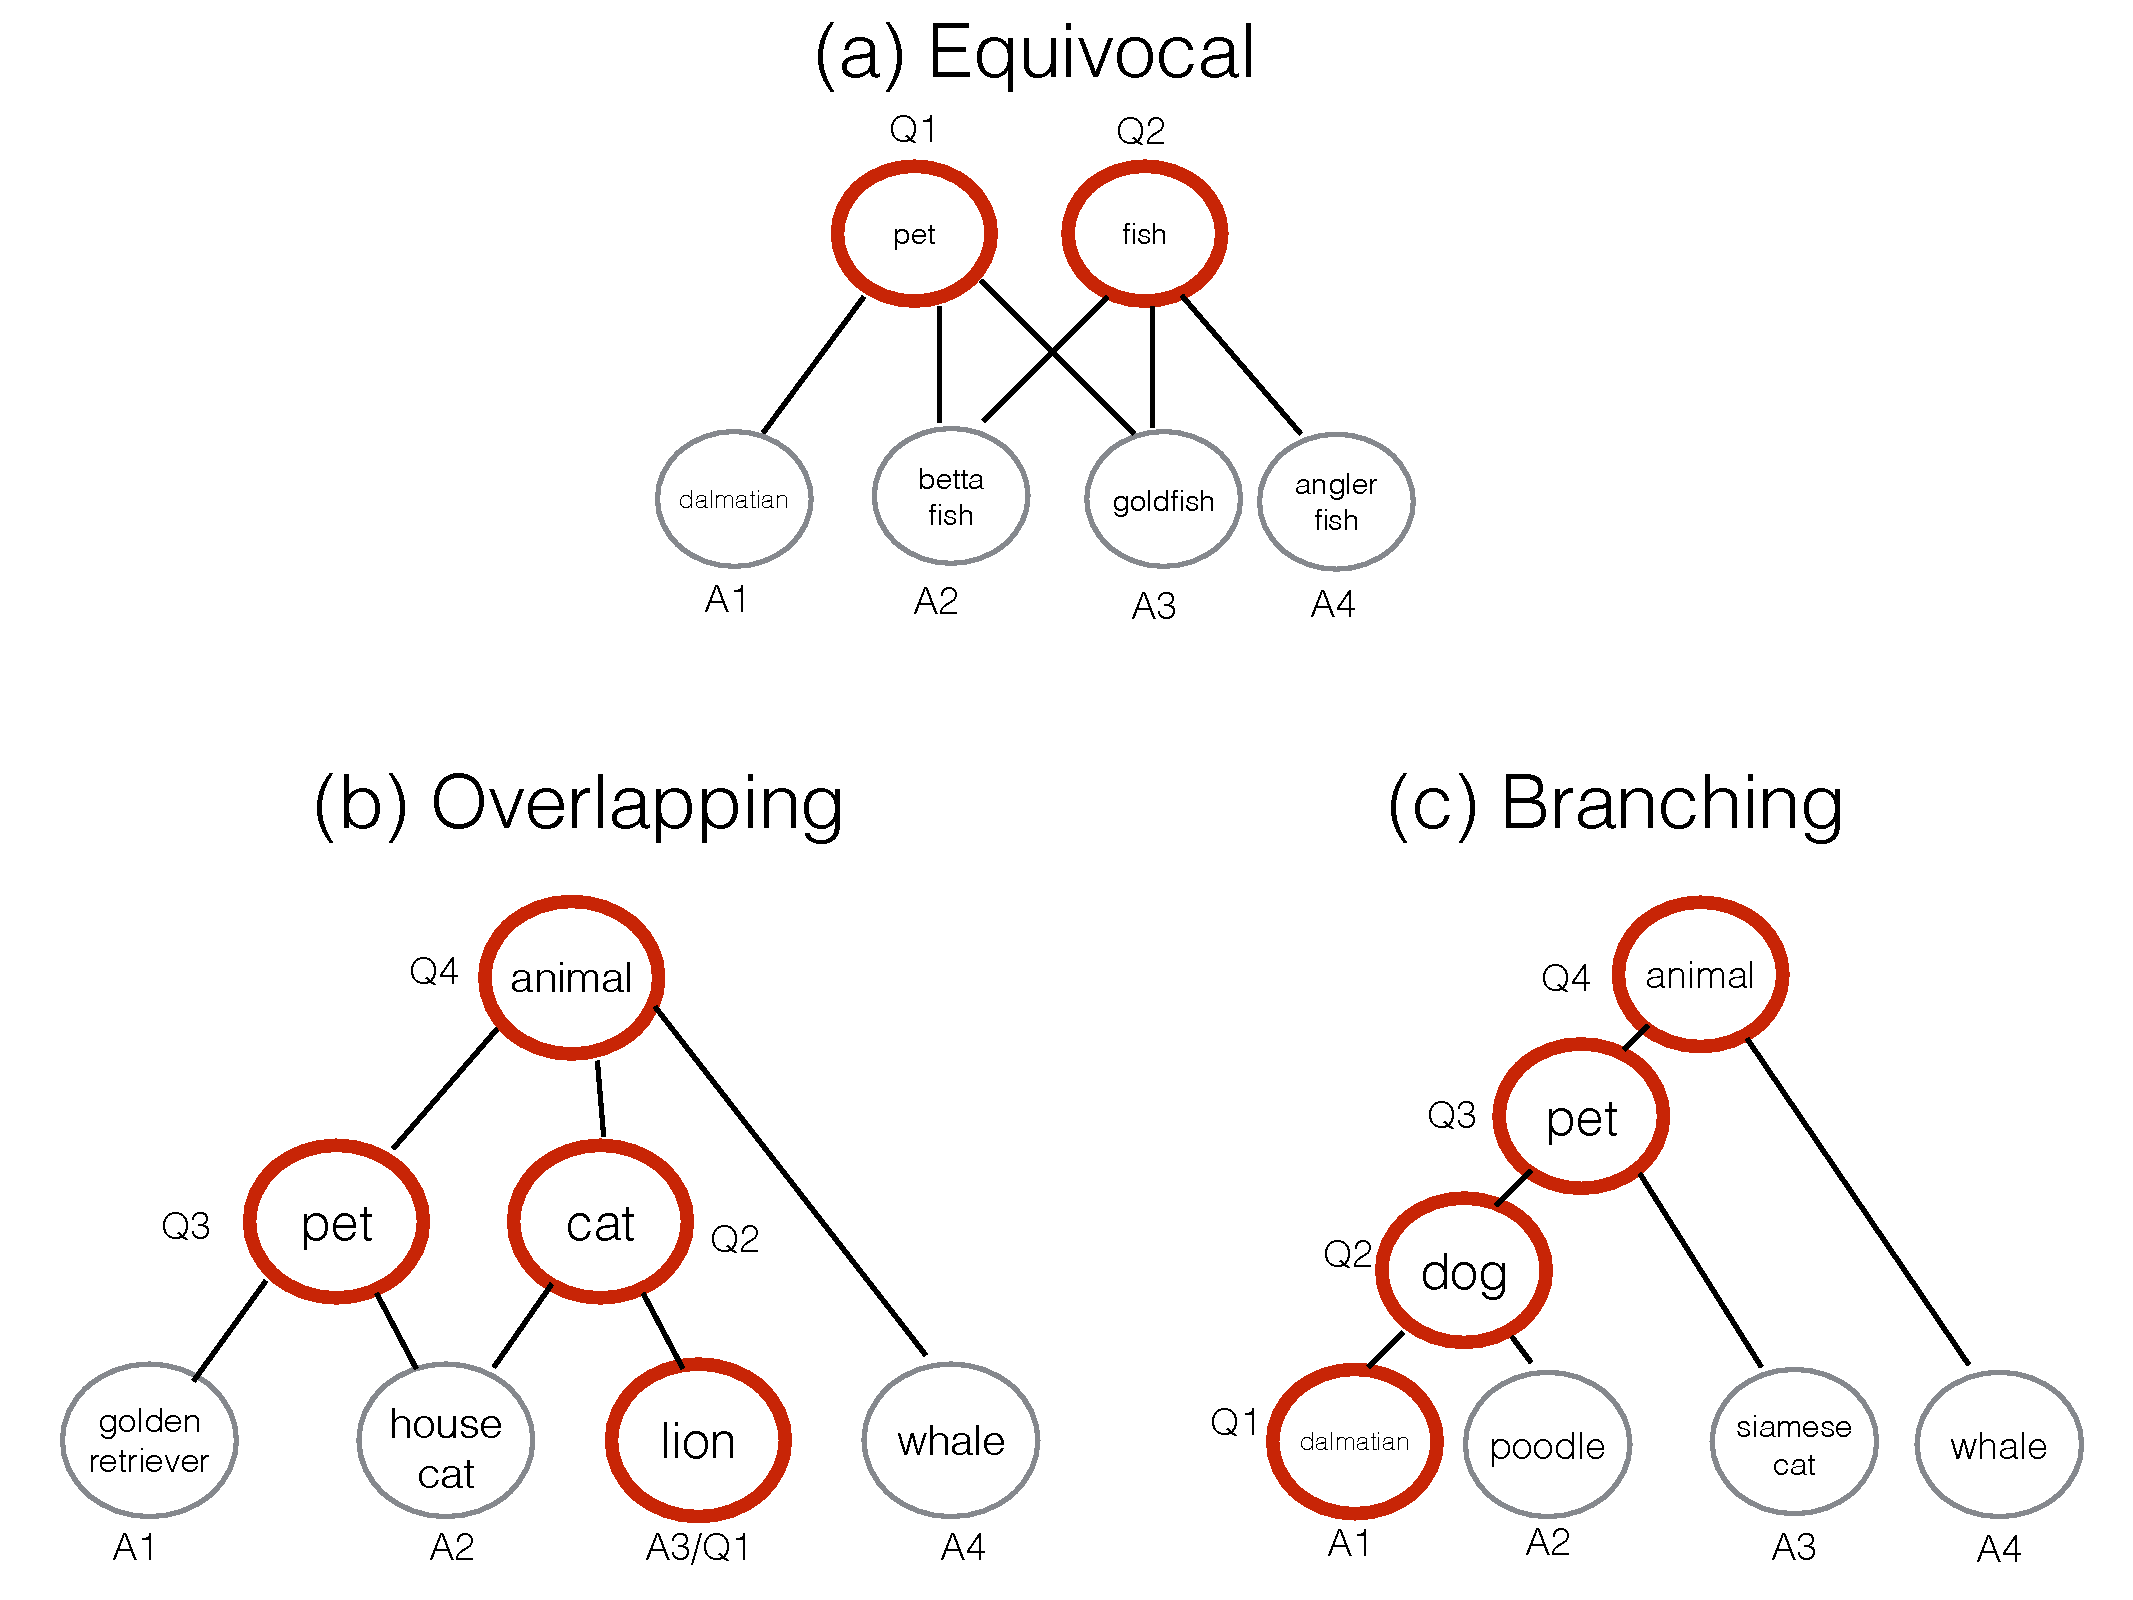
\includegraphics[scale = .5]{Exp1/hierarchyStructureExamples.pdf}
\end{center}
\caption{\footnotesize  Example of each type of conceptual hierarchy used in our experiment. The bottom row served as the goal and answer spaces, and the possible questions are highlighted in red. }
\label{fig:hierarchyStructures}
\end{figure*}
\section{Experiment 1: \\ Definite reference and salience}

%%%
As a first quantitative test of our models, we designed a cooperative guessing game that relies on knowledge of concept structure. 
% This game served as a minimal case of the Hidden Goal paradigm.
On each trial, four objects are hidden behind four doors.
One player -- the \emph{questioner} -- is assigned one of the objects to find as a private goal but does not know which object is behind which door (Fig. \ref{fig:expviews}A).
The other player -- the \emph{answerer} -- knows each object's true location but does not know which one the questioner is looking for (Fig. \ref{fig:expviews}B). 
To succeed in the face of this knowledge asymmetry, the questioner must first ask a question (i.e. \emph{where is the\dots?}), then the answerer must respond helpfully so that his partner can guess the location of her goal object more accurately (Fig. \ref{fig:expviews}C).

Critically, we manipulated the sets of goals, questions, and answers across trials to create a number of different scenarios where our models make distinguishable predictions.
To do so, we exploited the hierarchical conceptual structure provided by nominal referring expressions.
For example, a questioner could ask about the ``Dalmatian,'' ``dog,'' ``pet,'' or ``animal'' and all could plausibly be referring to a Dalmatian in the answerer's view \cite{Brown58_HowShallAThingBeCalled,GrafEtAl16_BasicLevel}. 
However, among these labels, only ``animal'' could truthfully refer to a whale.
This structure allowed us to introduce a family of indirect questions and answers by carefully selecting how the four objects are conceptually related to one another, and which questions are made available.

%These restrictions were motivated by one of the key features of indirect questioning: when the direct question (e.g. ``may I eat your food?'') is suppressed due to politeness, utterance length, complexity, or some other intervening factor, questioners instead rely on a pragmatic indirect question (e.g. ``are you going to eat that?''). 


\subsection{Methods}
\subsubsection{Participants} 
200 participants from Amazon's Mechanical Turk were recruited and paired into teams of two.
We excluded 50 participants due to a server crash that terminated the task before completion, and
excluded two additional games because participants reported that they were not native English speakers. 
This left 74 unique completed games (148 participants).

\subsubsection{Stimuli} 

To support quantitative model comparison, we needed to elicit graded behavior under a variety of different scenarios.
We thus constructed twelve items by crossing four conceptual domains (\emph{animals}, \emph{plants}, \emph{places}, and \emph{artifacts}) with three concept hierarchy structures (\emph{nested}, \emph{overlapping}, and \emph{equivocal}; see Figure \ref{fig:hierarchyStructures}).
Each item consisted of four objects and four labels, such that different labels referred to different subsets of objects at different levels of abstraction. 
The four objects served as possible goals and answers, while the labels served as possible questions\footnote{A document containing these mappings for all items, as well as their hierarchical relationships, is available online at \scriptsize\url{https://github.com/hawkrobe/Q\_and\_A/stimuliLabels.pdf}}.
The different concept hierarchy structures were intended to serve as conditions driving qualitatively different model predictions, while the conceptual domains were intended to support item-level generalizability within each condition.

%The objects in context on a given trial belong to a conceptual hierarchy (see Fig. \ref{fig:hierarchyStructures} for several examples).
%As discussed in detail below, our models make qualitatively and quantitatively different predictions about (1) which of these levels the questioner will choose in different contexts and (2) how answerers will respond to underspecified questions like ``Where is the dog?'' when there are multiple dogs in context.

\subsubsection{Procedure}

\begin{figure*}[h]
\begin{center}
\includegraphics[scale = .9]{Exp1/QualitativePredictions.pdf}
\end{center}
\caption{\footnotesize  Qualitative model predictions and results for (A) answerers in nested condition and (B) questioners in overlapping condition. Highlighted rows indicate clearest qualitative differences. Labels shown from `animals' domain; response counts aggregated across all four domains.}
\label{fig:exp1qualitative}
\end{figure*}

After passing a short comprehension quiz on the game instructions, participants were randomly assigned to the role of questioner or answerer and paired with another participant in a shared virtual environment using the infrastructure described in \citeA{Hawkins15_RealTimeWebExperiments}. 
Some aspects of each participant's environment were denoted as private (i.e. the questioner's goal and the answerer's knowledge of object locations) while others were explicitly flagged as common ground (i.e. the sets of possible questions and objects).
%The questioner and answerer interfaces are displayed in Figure \ref{fig:expviews}. %Information was presented on the left side of the screen, and players used the right side as a workspace to view goals, ask questions, and respond with answers. 
%It was important to sets were presented alternatives are fixed and held in common ground for all participants. 
Fixing these sets and making them explicit as common ground allowed us to avoid ad hoc assumptions about these sets in our model formulation, and also reduced the memory load on participants.


We constructed the trial sequence such that each participant provided one response for each of the twelve items, in a random order.
Each trial proceeded through four phases. 
First, the questioner was randomly assigned one of the four possible goals by a spinning wheel animation.
They then used a drag-and-drop interface to select one of the four questions to send.
Upon seeing this question appear, the answerer responded with a location (``The X is behind door Y'') by dragging the object they wanted to reveal into a box. 
Each of these drag-and-drop actions was rendered for the other participant in real time to emphasize that they were playing with a real human partner.
Finally, after receiving the answer, the questioner clicked on one of the gates to make their guess. 
Both players received feedback about the outcome of the guess: the questioner saw the true locations of the objects, and the answerer saw the true goal. 

\subsection{Qualitative behavioral predictions}

Before proceeding to quantitative model comparisons, we highlight several key patterns in the behavioral data where models make qualitatively different predictions. 
Because there was high pairwise correlation $(r = 0.91 \textrm{ to } 0.97)$ in response probabilities among different domains for both questioners and answerers\footnote{with the exception of the `place' domain in answerers, which is likely due to a confusing choice of object images ($r = 0.78$; see Supp. Table \ref{table:experiment4correlations})}, we pool response counts across domains.
For readability, we continue using examples from the ``animal'' domain when reporting these qualitative results.

\subsubsection{Answerer behavior}
The most straightforward qualitative prediction distinguishing our answerer models concerns the \emph{nested} condition. 
This condition was characterized by four successively more specific labels, ranging from the super-ordinate ``animal'' to the sub-ordinate ``Dalmatian.'' 
At each layer of conceptual nesting, one of the objects in context was excluded: ``animal'' is true of all four objects, ``pet'' is true of three, and so on.
Thus, some answerer behavior is obvious and predicted by both $A_1$ and $A_2$: when asked ``Where is the \emph{Dalmatian}?'', 100\% of participants revealed the location of the Dalmatian.

Other questions, however, lead to sharp qualitative differences.
Suppose the questioner asks ``Where is the \emph{animal}?''. 
Neither $A_0$ nor $A_1$ have a preference over which of the animals to provide information about, because all four satisfy the literal meaning of the question. 
Human participants, on the other hand, have a strong preference: 94\% provided the location of the ``whale,'' the object that isn't queried by any of the other questions, $\chi^2(3) = 210.8, p < 0.001$ (see Fig. \ref{fig:exp1qualitative}A).

This strong non-uniform pattern %, also found by \citeA{HawkinsStuhlmullerDegen15_qAndA}, 
is only consistent with $A_2$. 
To understand this, consider the Gricean inference that can be made about the underlying goal from the utterance ``Where is the animal?''
$A_2$ reasons that if the questioner were looking for the Dalmatian, they would be more likely to ask ``Where is the Dalmatian?'' 
If looking for the other dog, the poodle, they would have asked ``Where is the dog?''
More generally, they would have been more likely to ask a more direct question under any goal except the ``whale'', and the fact that they \emph{didn't} ask one of these more direct questions is evidence that they didn't have these goals.
Having inferred that the most likely goal is the whale, $A_2$ gives the most informative, relevant answer: the location of the whale.

\subsubsection{Questioner behavior}
Next, we turn to a subtler qualitative pattern in the ``overlapping'' condition, which was specifically designed to distinguish between our \emph{questioner} models. 
Suppose the questioner is assigned the ``house cat'' as their goal object. 
What question do they ask? 
$Q_0$ is equally likely to ask any of the four questions, since $A_0$ ignores their utterance anyway. 
$Q_1$, in turn, is evenly split between the two parents in the tree -- ``Pet?'' and ``Cat?'' -- since $A_1$ would have a 50\% chance of responding with the house cat's location in either case. 

$Q_2$, however, takes into account the goal inferences $A_2$ would make after hearing her question. 
Once $A_2$ hears ``Cat?'' he will infer, using the same Gricean logic described above, that because the more specific ``Lion?'' is an available alternative for the questioner, she would have \emph{directly} asked about it if it were her goal. 
Because she didn't, he infers that she must be interested the other cat (her true goal). 
``Pet?'' on the other hand, gives no clue to her goals and is therefore less preferred. 
Thus, we have a pair of sharply distinguishable predictions: $Q_0$ predicts all four questions will be equally likely, $Q_1$ predicts that ``Pet?'' and ``Cat?'' will be equally likely, and $Q_2$ predicts an asymmetry where ``Cat?'' is the preferred question.

%
%\begin{figure}[t!]
%\begin{center}
%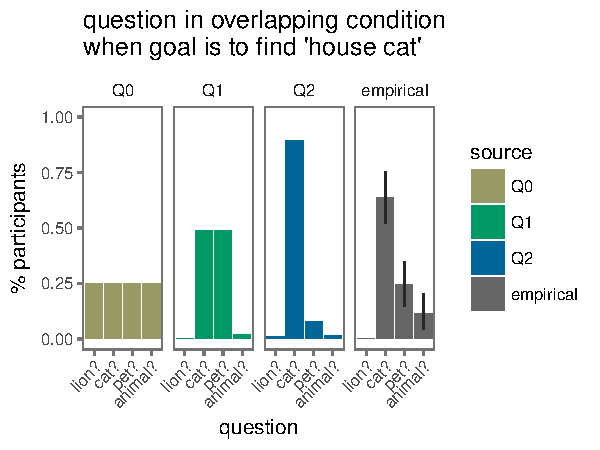
\includegraphics[scale=.9]{OverlappingModelComparison.pdf}
%\end{center}
%\caption{.}
%\label{fig:Exp4ZoomedIn}
%\end{figure}

The counts of participants asking each possible question in this scenario, collapsed across domains, is shown in Fig. \ref{fig:exp1qualitative}B. 
We find that the pragmatic model $Q_2$ makes the correct qualitative prediction -- the empirical probability of asking ``Cat?'' ($\hat{p} = 0.64$) is significantly different from the  probability of asking ``Pet?'' ($\hat{p} = 0.25$; bootstrapped $95\%$ CI on difference: $[0.17, 0.58]$). 
This critical condition thus provides qualitative evidence for $Q_2$: in some cases, questioners consider the answerer's inference about their goals when selecting their question. 

%Thus, in examining the results below we will collapse across domains for simplicity of analysis. 
%Still, it is worth noting that the ``place'' domain has the lowest inter-domain correlations for both questioners and answerers, indicating that it may be an outlier -- we will return to this point in the discussion below.  Next, we step through the response patterns for each hierarchy type. For concreteness, though all statistical tests were conducted on data pooled across domains, we report our results in terms of the `animal' domain instead of the abstract goal, question, and answer labels (see Figure \ref{fig:exp4res} for the full response distributions).
%
%\begin{figure*}[t!]
%\begin{center}
%\includegraphics[scale = .75]{Exp2QuestResults}
%\includegraphics[scale = .75]{Exp2AnsResults}
%\end{center}
%\caption{Results and model fits, for the best-performing questioner (left) and answerer (right) models, collapsing over the different domains. Error bars represent bootstrapped 95\% confidence intervals.\todo[inline]{Judith: axes difficult to read. Maybe just use animal labels here? Or move to supplemental?}}
%\label{fig:exp4res}
%\end{figure*}

%In the `overlapping' condition (Figure \ref{fig:hierarchyStructures}(b)), questioners preferentially asked about the `lion' when looking for the lion, $\chi^2(3) = 205, p < 0.001$; about the `cat' when looking for the Siamese cat, $\chi^2(3) = 63, p < 0.001$, even though the lion is also a cat; about the `pet' when looking for the dalmatian, $\chi^2(3) = 232, p < 0.001$, even though the Siamese cat is also a pet; and about the `animal' when looking for the whale, $\chi^2(3) = 213, p < 0.001$. Answerers preferentially revealed the lion when asked about the `lion,' $\chi^2(3) = 229, p < 0.001$, the Siamese cat when asked about the `cat,' $\chi^2(3) = 59, p < 0.001$, the dalmatian when asked about the `pet,' $\chi^2(3) = 120, p < 0.001$, and the whale when asked about the `animal,' $\chi^2(3) = 187, p < 0.001$. 

%In the `branching' hierarchy (Figure \ref{fig:hierarchyStructures}(c)), we found that questioners strongly prefer to ask about the `dalmatian' when trying to find the dalmatian, $\chi^2(3) = 190, p < 0.001$, about the `dog' when trying to find the poodle, $\chi^2(3) = 152, p < 0.001$, about the `pet' when trying to find the siamese cat, $\chi^2(3) = 168, p < 0.001$, and about the `animal' when trying to find the whale, $\chi^2(3) = 210, p < 0.001$. %Answerers respond in kind. , and in an earlier version of the multi-player study we report in this section.

To summarize, our non-pragmatic models cannot account for key qualitative phenomena while our pragmatic models ($A_2$ and $Q_2$) make the correct predictions. 
Next, we show that our pragmatic models also provide better overall quantitative fits to the raw behavioral data. 
Before describing the results of our model comparison, we formalize the task setup in our modeling framework. 

\subsection{Quantitative model comparison}

\begin{figure*}[tbh!]
\begin{center}
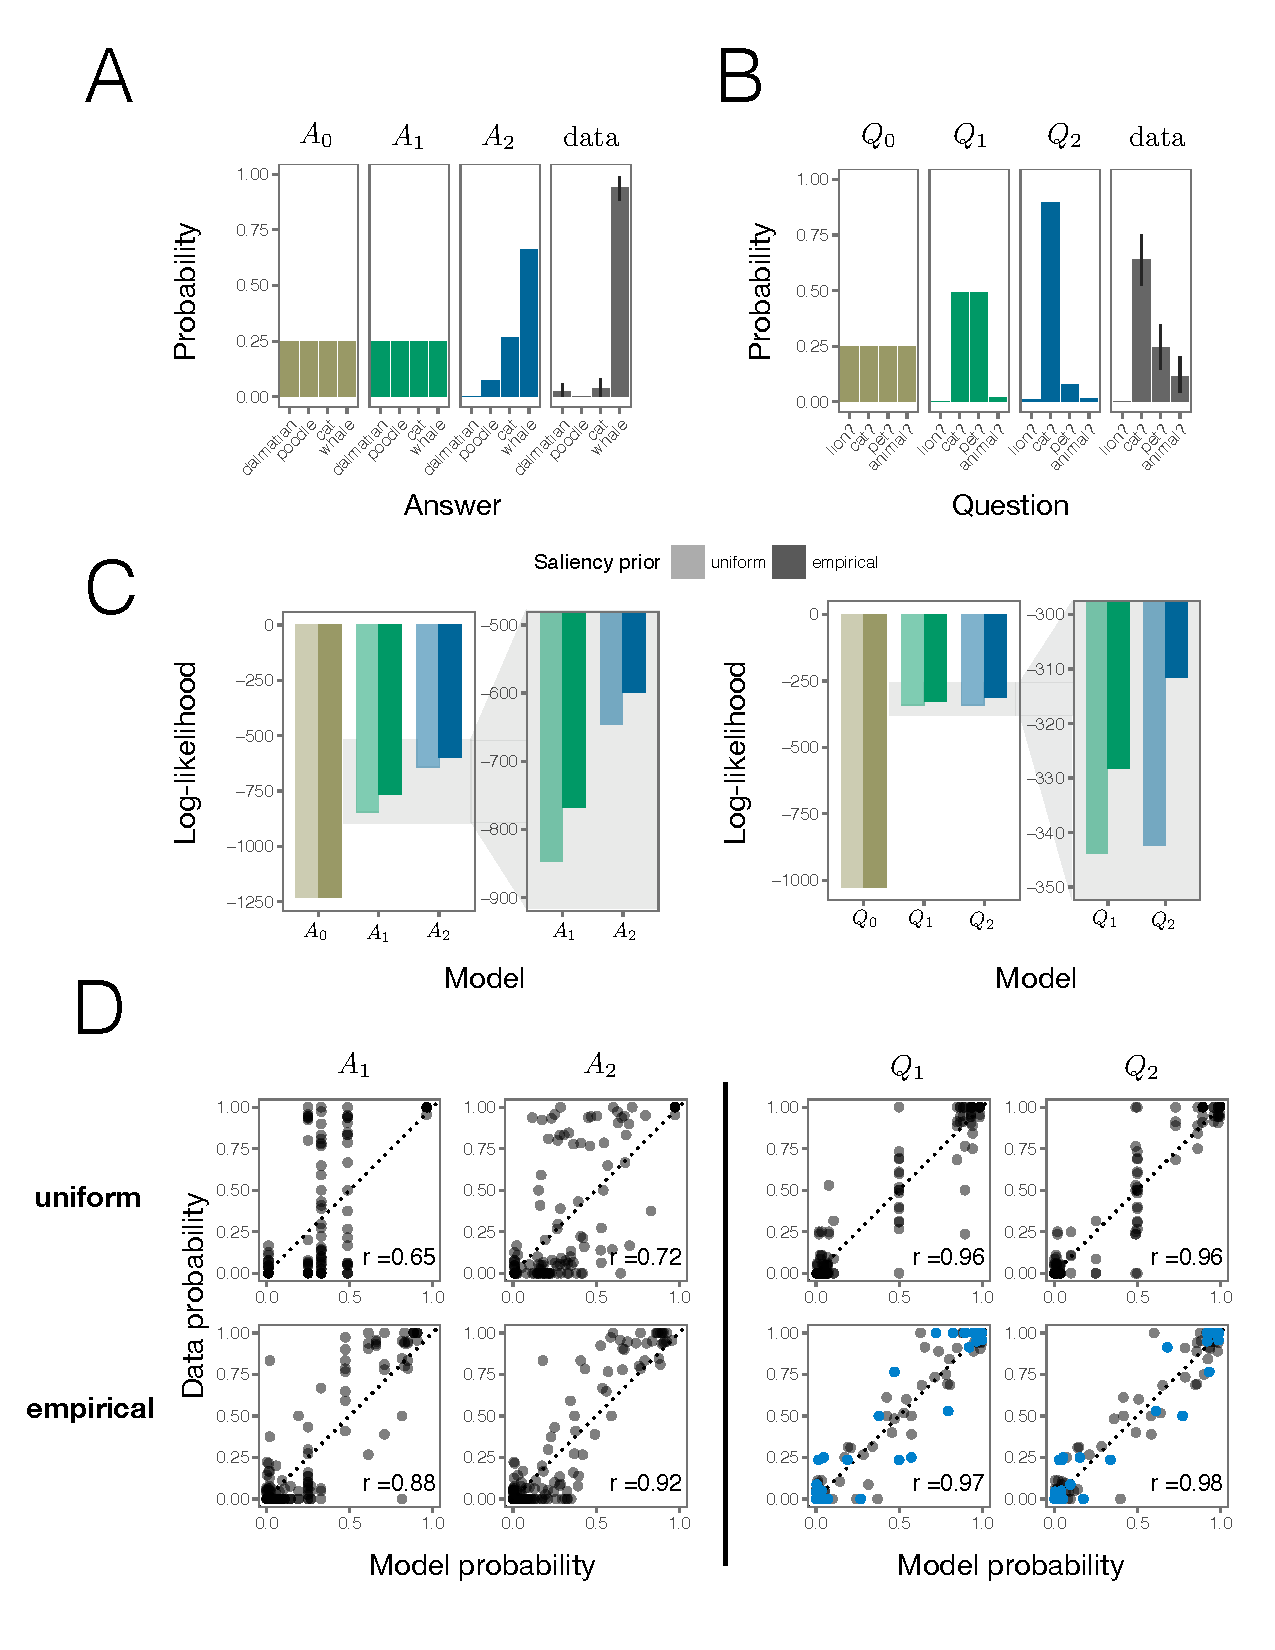
\includegraphics[scale = .77]{Exp1/ResultsFig.pdf}
\end{center}
\caption{Posterior predictives for each model, which indicate good overall fit (excluding $A_0$ and $Q_0$). Blue dots on $Q$ plots indicate overlapping condition.}
%\vspace{-1cm}
\label{fig:exp1predictives}
\end{figure*}

% Please add the following required packages to your document preamble:
% \usepackage{booktabs}
% \usepackage{multirow}

\subsubsection{Setup} 
Corresponding to the structure of our experiment design, we take the set of possible worlds $\mathcal{W}$ on a given trial to be the set of possible permutations of the four objects to the four locations (yielding $4! = 24$ possibilities). 
Because we explicitly instructed questioners to find the location of a particular object, we then take the space of goals $\mathcal{G}$ to be the set of goal projections $$g_o(w) = \textrm{loc}(o,w)$$ where $\textrm{loc(o,w)}$ is a simple function looking up the location of object $o$ in world $w$. 
Similarly, the answer space $\mathcal{A}$ is the set of constructions ``The $o$ is behind gate $i$.'' which evaluate to true in worlds where $o$ is at location $i$ and false otherwise.
We assume uniform prior probability over worlds, goals, questions, and answers. 

%The formal semantics of the questions in our experiment  several classic problems in linguistics.
%The semantics of questions in this domain is 
%To populate our question space $\mathcal{Q}$, we must specify the explicit meaning of the question ``Where is the $x$?'' for each of the four labels allowed in a given trial (see Fig. \ref{fig:hierarchyStructures}). 
Specifying the formal semantics of the question space $\mathcal{Q}$ draws upon several results from linguistics. 
The denotation of a noun phrase containing a definite article is only defined if there is a unique, salient object that the noun picks out in the world; pragmatically, then, the use of a definite article \emph{presupposes} the uniqueness or salience of some object in shared context \cite{Lewis79_Scorekeeping, clark1983common, Roberts03_UniquenessDefiniteNounPhrases}. 

Thus we take the literal meaning of each question $q$ to be: 
$$\textrm{\den{Where is the x?}} = q_{x}(w) = \textrm{loc}(s_x,w)$$ where $s_x$ is the \emph{salient} object of category $x$. 
In contexts where there are multiple objects of category $x$, the question is interpreted by drawing an object from a prior saliency distribution, given the category in the noun phrase: $s_x \sim \mathcal{S}(o | x)$. 
This distribution may depend on typicality for the category \cite{Rosch75}, world knowledge about what labels people tend to use to refer to different objects, and so on. 

\subsubsection{Eliciting saliency priors}
In prior work, there have been two approaches to setting such model-internal prior distributions in a principled manner.
The first is to treat these internal distributions as additional free parameters and jointly infer them from the behavioral data along with other parameters of interest \cite<e.g.>{TesslerGoodman16_Generics, tauber2017bayesian}. 
The second is to use an independent task to empirically elicit these priors from a separate population of participants, and then use this (parameter-free) distribution in the model \cite<e.g>{KaoWuBergenGoodman14_NonliteralNumberWords}.
Here, we take a hybrid approach. 
We elicit empirical saliency priors from an external sample, as in the second approach, but then infer the extent to which these empirical priors are actually necessary for explaining participants' question and answer behavior in our model comparison.

We thus designed a simple language saliency elicitation task using the stimuli from our communication task.
On each trial, we presented participants with a set of four pictures and a label $X$ and were asked to ``Click \emph{the} $X$.''
Each participant was given one trial for each of the twelve items used above; to obtain the label $X$, we sampled one of the four possible category nouns that could be used in questions. 
In this way, no participant saw the same set of objects more than once. 
%The order of trials and positions of pictures within trials were randomized.
Of 192 participants recruited from Amazon's Mechanical Turk, 13 participants were excluded after reporting a non-English native language, and 15 more were excluded due to self-reported confusion over the instructions. 
This left data for 164 participants.
To form an empirical saliency distribution $s_x \sim \mathcal{S}(o | x)$ that can be used in the model, we computed the proportion of participants that clicked on each of the objects $o$ for each label $x$. 

Before formally testing the usefulness of these empirical saliency estimates in our model comparison, we conducted a simple test of the null hypothesis that participants use a uniform saliency prior over within-category objects when interpreting the definite article. 
We performed $\chi^2$ goodness of fit tests on the response distribution for each label: a total of 32 tests. 
We found that 69\% of these tests rejected the null hypothesis of uniformity at a (Bonferroni-corrected) significance level of $\alpha = 0.05/32 = 0.002$ indicating that saliency distribution often deviates from uniform.

\subsubsection{Results of model comparison}
\begin{table}[]
\begin{center}
\begin{tabular}{@{}llrr@{}}
\toprule
 &  & \multicolumn{1}{l}{\begin{tabular}[c]{@{}l@{}}uniform\\ saliency\end{tabular}} & \multicolumn{1}{l}{\begin{tabular}[c]{@{}l@{}}empirical\\ saliency\end{tabular}} \\ \midrule
\multirow{3}{*}{\begin{tabular}[c]{@{}l@{}}answerer\\ models\end{tabular}} & $A_0$ & -1231.0 & -1231.0 \\ \cmidrule(l){2-4} 
 & $A_1$ & -847.5 & -767.2 \\ \cmidrule(l){2-4} 
 & $A_2$ & -645.7 & \textbf{-599.6} \\ \midrule
\multirow{3}{*}{\begin{tabular}[c]{@{}l@{}}questioner\\ models\end{tabular}} & $Q_0$ & -1025.9 & -1025.9 \\ \cmidrule(l){2-4} 
 & $Q_1$ & -343.8 & -328.3 \\ \cmidrule(l){2-4} 
 & $Q_2$ & -342.3 & \textbf{-311.5} \\ \bottomrule
\end{tabular}
\vspace{1em}
\end{center}
\caption{\footnotesize Results of quantitative model comparison; marginal likelihoods shown on log scale.}
\label{tab:exp1likelihoods}
\end{table}

%How does correcting this assumption affect our quantitative model predictions? 
%The empirical saliency distributions we collected can be directly substituted in for $\mathcal{S}(o|x)$ when defining the literal semantics of ``Where is \emph{the}\dots?'' questions. 


%We assume uniform prior probability over worlds, goals, questions, and answers. 
%This finishes the specification of the three Questioner models and three Answerer models for our experimental situation.
For a rigorous model comparison among our different questioner and answerer models, we conducted a Bayesian data analysis \cite{LeeWagenmakers14_BDA}. 
We introduce a discrete hyperparameter $\gamma \in \{0, 1, 2\}$  determining which model to use, and jointly infer this parameter along with the continuous rationality parameter $\alpha$.
Additionally, to test whether a model using our non-uniform empirically-measured saliency distribution provides a better fit to the data, we add an additional parameter $\beta$ which interpolates between a uniform salience prior ($\beta = 0$) and the empirical salience distribution we measured ($\beta = 1$). 
In other words, we assume participants use some mixture between the pure uniform and empirical saliency and we infer the mixture weight.
We place uninformative priors over these parameters,
$\gamma \sim  \textrm{unif}\{0, 1, 2\}$ and 
$\alpha   \sim  \textrm{unif}(0,20)$, 
$\beta \sim \textrm{unif}(0, 1)$
and performed inference using enumeration over discrete bins. 

After marginalizing over values of $\alpha$ and $\beta$, the posterior $P(\gamma | \textrm{data})$ can be interpreted as the relative evidence for each model \cite{KruschkeVanPaemel15_OxfordHandbook}.
Results are shown as marginal likelihoods in Table \ref{tab:exp1likelihoods}. 
We can immediately rule out $A_0$ and $Q_0$, which predict a uniform distribution of responses within each condition and performed many orders of magnitude worse than the other models.
Among the remaining answerer models, we found overwhelming evidence for $A_2$ relative to $A_1$ (BF~$\approx~6~\times~10^{72}$). 
For our questioner models, we found substantial evidence for $Q_2$ relative to $Q_1$ (BF~$\approx2\times~10^{7}$). 

Next, having established support for $A_2$ and $Q_2$, we test the extent to which the introduction of empirical saliencies improved our predictions. 
Again using Bayes Factors, which automatically penalize our empirical saliency model for its additional flexibility, we found strong evidence against the $\beta=0$ model for both the answerer (BF = $1.12\times 10^{20}$) and questioner ($2.44 \times 10^{13}$), suggesting that participants interpret questions using non-uniform saliencies.
Finally, the posterior predictives for $A_2$ and $Q_2$ after including empirical saliencies explain a substantial proportion of the item-wise variance: $R^2 = .92$ and $R^2 = .98$, respectively (see Fig. \ref{fig:exp1predictives}). %Posteriors over alpha are similar to our previous results. \ndg{Appendix}% (see Appendix).


%
%\begin{figure*}[t!]
%\begin{center}
%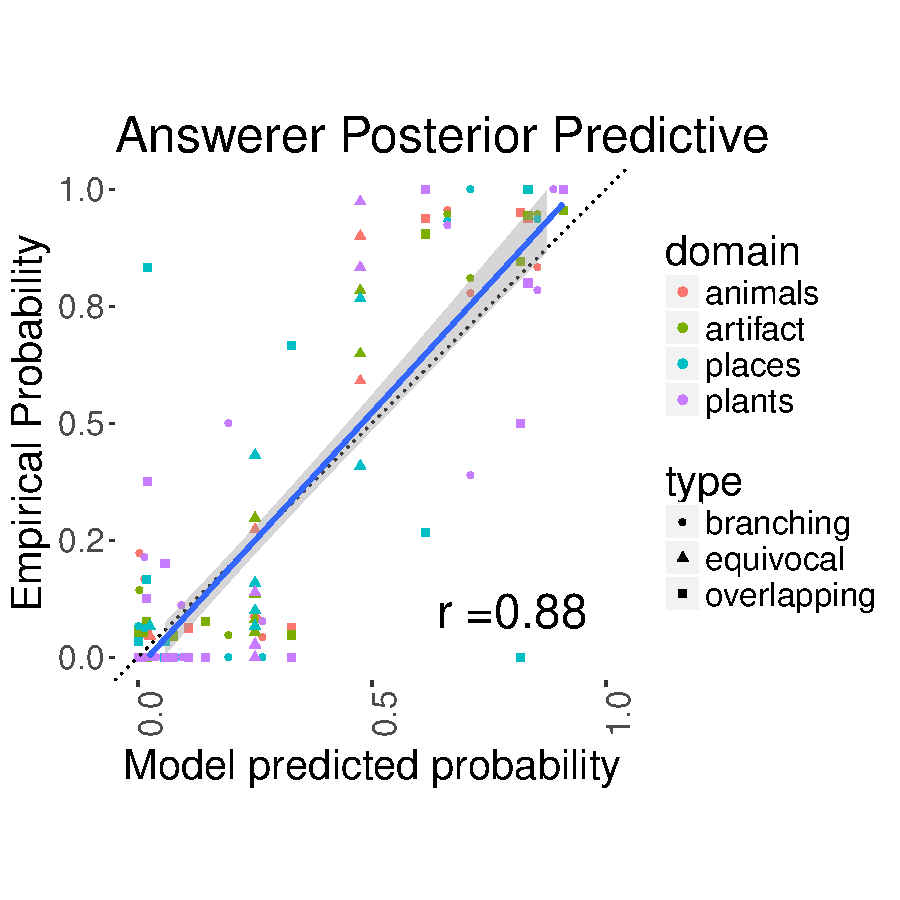
\includegraphics[scale=.5]{betaZeroAnswerer_Predictives}
%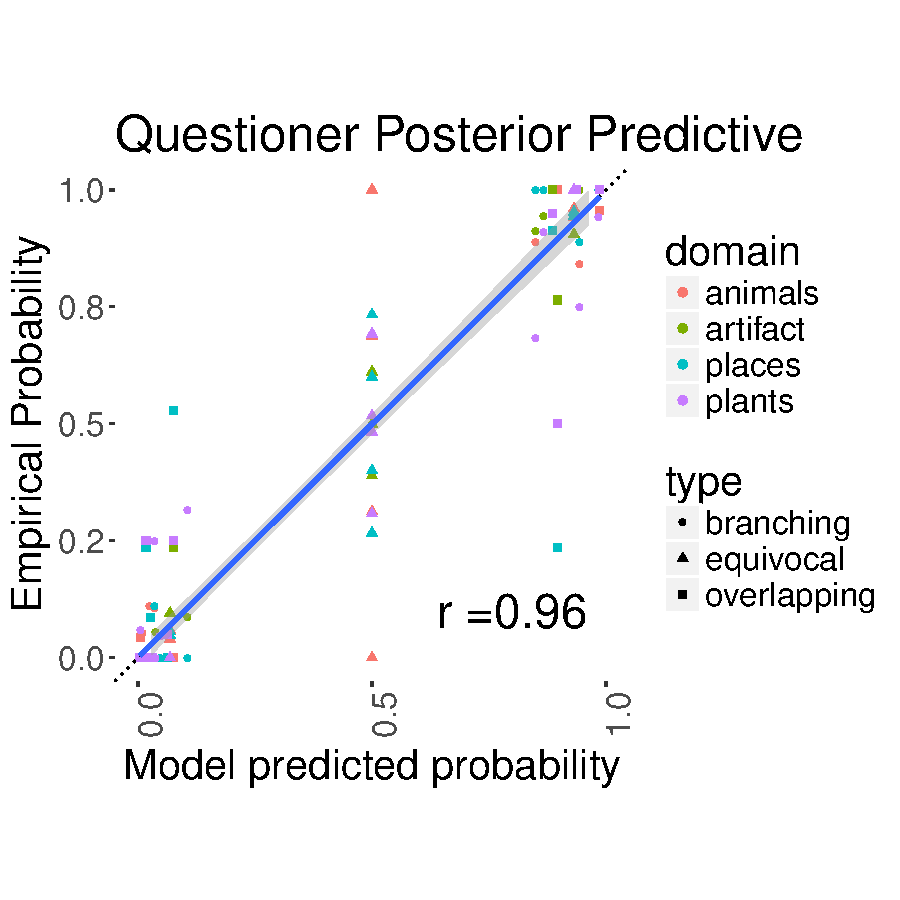
\includegraphics[scale=.5]{betaZeroQuestioner_Predictives}
%\end{center}
%\caption{Full space of models, and their correlations with the data, broken down by item and type.}
%\label{fig:answererPredictives}
%\end{figure*}


%

%

%\subsection{Discussion}

%%We also identified four shortcomings of Experiment 1. First, despite the success in distinguishing between answerer models, our data are not sufficient to distinguish between the explicit and pragmatic \emph{questioner} models. The two models did not make significantly different predictions for this experiment (and both are sufficient to account for the data). 
%
%
%

%First, we found additional evidence that $A_2$ answerer can account for essential qualitative features of the response data. For example, the explicit answerer predicts a uniform distribution over responses to the `animal?' question in the branching hierarchy. All four of the objects are animals and under the assumption that all four are equally salient, the question meaning projection is equally likely to pick out any of them. Contrary to these predictions, we found that answerers overwhelmingly preferred the response ``whale'' to the other three responses, which is accurately predicted by the Gricean dynamics of the pragmatic model. If the questioner were interested in any animal other than the whale, they would have asked a different question; since they didn't, they must have meant the whale. Like our final case study, this task required the answerer to use the questioner's utterance as a signal of their underlying goals.

%Additionally, we were able to test the predictions of the \emph{questioner} component of the model for the first time. We found that at an aggregate level, both $Q_1$ and $Q_2$ accurately predict what questions an agent will pick when faced with a particular goal. However, our results for the overlapping hierarchy in particular show that the pragmatic model is necessary to account for some critical aspects of the data. 

%% NOTE ABOUT OUTLIER, if necessary... 
%The ``place'' domain that we flagged as a potential outlier earlier in the results is the only domain that does not show the pattern of responses predicted by the pragmatic questioner model. This is likely due to the choice of images displayed to participants: the two ``parent'' nodes of the critical goal are ``bar'' and ``restaurant,'' and we represented the intersection of these two categories as a hotel lobby. However, the image we chose placed emphasis in the bar in the hotel, which likely biased participants toward the ``bar'' response instead of the ``restaurant response'' predicted by the pragmatic model. 

%Finally, we made certain assumptions in modeling our hierarchies, such as the assumption that participants do not consider whales to be pets despite the fact that it's technically possible. 

%We address these issues by collecting independent estimates of participants' saliency knowledge in interpreting definite articles. 
%We then recompute our model's predictions using empirical saliency priors, in place of our previous assumption of uniform saliency within a category. We conduct a new Bayesian data analysis using these new predictions to test (1) whether our models more appropriately capture item-level variability and (2) whether the pragmatic models still provides a better fit after controlling for typicality knowledge.

\subsection{Discussion}

%In three case studies, we first established that among our answerer models only $A_2$, which goes beyond the literal meaning of the question to infer and address underlying \emph{goals}, could account for classic qualitative answerer-sensitivity effects. 
In Experiment 1, presented both answerer and questioner models with the  \emph{quantitative} challenge of accounting for trial-level variance in a Hidden Goal task. 
We found strong converging support for $A_2$ relative to our other answerer models and, for the first time, tested the predictions of our questioner models. 
While both $Q_1$ and $Q_2$ provided good predictive fits to our question-asking data, only $Q_2$ could account for asymmetries in the critical \emph{overlapping} condition and was therefore also preferred in a Bayesian model comparison. 
We also found that incorporating realistic saliency priors to interpret definite questions provided a substantially better fit to our data. 

There are two reasons incorporating typicality into our model is important. 
First, failures to account for typicality could potentially invalidate the conclusions of our model comparison. 
For example, we expect a house cat to be a much more typical exemplar of the category `cat' than a lion. 
Hence, participants may not be choosing the house cat in this item for pragmatic reasons; they may just be selecting the more salient member of the category. 
If this were the case, including saliency knowledge should improve the predictions of $A_1$ and $Q_1$, thus potentially `explaining away' any benefit of deeper pragmatics. 
After accounting for this potential confound, we still found strong evidence for $A_2$ and $Q_2$ over simpler models.

Second, Fig. \ref{fig:exp1predictives} makes it clear that without these saliencies, $A_2$ and $Q_2$ fail to capture graded responses across different domains. 
This is especially striking in the `equivocal' condition where our models predict no preference in questioner behavior: if asking about the goldfish, which is both a ``pet'' and a ``fish,'' then the symmetry of the alternatives provides no reason to favor one label over the other. 
Instead, we found a high degree of variability across domains. 

For example, when questioners were trying to find a pet goldfish, 85\% of participants preferred the label `fish' to the label `pet,' even though both are technically true. 
In the `artifacts' domain, on the other hand, questioners had no preference between asking about the `seat' or `metal thing' when the objects (metal chairs) fell into both categories.
To understand how our empirical saliency distribution captured this data, consider that a Dalmatian is a far more typical and salient member of the `pet' category than a goldfish \cite{Rosch75}. 
Hence a questioner considering this knowledge as common ground would know that asking ``Where is the pet?'' would tend to elicit information about the Dalmatian, not the goldfish. 
If they were looking for information about the goldfish, they would then prefer to ask about the `fish' category, where a goldfish is a highly typical example. 
In these cases, saliency strongly guides interpretation of the definite article in questions.

Our model for Experiment 1 also served as a first demonstration of the ``compositionality'' of our computational framework with other formal proposals in linguistics and cognitive science.
Because our model framework derives question and answer pragmatics given more elemental choices of literal question and answer semantics, world states, and goals, we could neatly accommodate definite reference and salience in questions by importing formal semantic proposals for definiteness developed in linguistics and philosophy.
In other words, the core computational framework itself did not need to be extended, only applied to the appropriate space of questions. 
In Experiment 2, we design a more targeted experiment to test our pragmatic questioner $Q_2$ and show that our model can similarly accommodate more structured \emph{goals}.

\section{Experiment 2: Structured goals}

The construct of a goal has a long history in psychology \cite{miller1960plans, Schank:1977hh, austin1996goal}.
The simplest spaces of goals, like those used in Experiment 1, are discrete sets of projections on the world state.
For example, in the Stroop task commonly used to study cognitive mechanisms of goal-directed behavior, the goal is either to (1) read the presented word or (2) name the color in which they are written \cite{miller2001integrative}.
However, for more complex behaviors, it is often useful to represent goals in \emph{hierarchically structured} spaces \cite{badre2008cognitive,botvinick2008hierarchical}. 
We often need to achieve multiple subgoals in pursuit of a larger, more abstract goal. 
These more structured representations have also been key to explaining third-party goal inferences in Bayesian models of theory of mind \cite{BakerSaxeTenenbaum09_ActionUnderstandingInversePlanning}. 
For example, if we know an agent takes the same route home every day, but one day we observe them veering off of this route toward the grocery store, we simply infer that they intend to run this errand as a subgoal of their ultimate goal of getting home. 

The hierarchical structure of goals has also long been recognized in linguistic theories of questions in discourse  \cite{Kuppevelt95_TopicalityDiscourse,Roberts96_InformationStructureDiscourse,Buring03_DtreesBeansBaccents,Groenendijk99_LogicOfInterrogation,rojas2014discourse}.
For instance, if a traveler asks \emph{Are there window seat tickets to Berlin at 7:00?} and there are no such tickets available, it would be more helpful for the travel agent to respond \emph{the next available tickets are for 10:00} than \emph{no} \cite{rojas2013roadsigns}.
This has been understood as a recognition by the agent that the specific flight and seat preference mentioned by the traveler are subgoals in a hierarchy below the broader goal of getting to Berlin. 

Structured goals of this type are naturally accommodated by our framework. 
To show this, we designed a simple Hidden Goal collection game inspired by recent experiments in multi-task reinforcement learning \cite{oh2017zero, andreas2017modular}.
Furthermore, this task presented the opportunity to more strongly test the pragmatic questioner model $Q_2$.

\begin{figure*}[tbh!]
\begin{center}
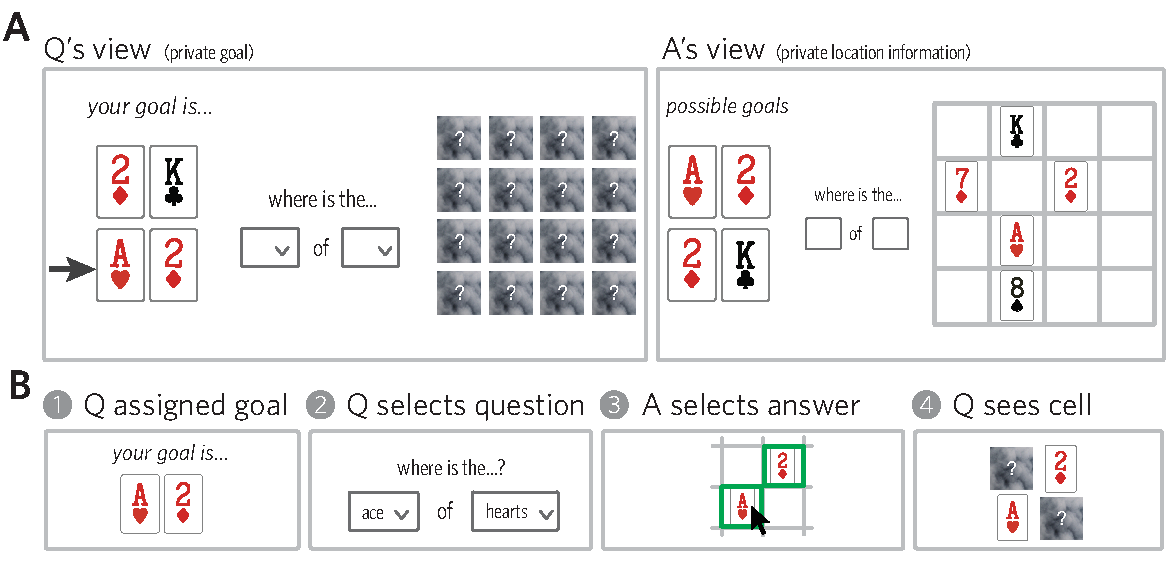
\includegraphics[scale = .7]{Exp2/task.pdf}
\end{center}
\caption{(A) Task displays and (B) procedure for Experiment 2.}
%\vspace{-1cm}
\label{fig:exp2task}
\end{figure*}


As in Experiment 1, participants were either assigned the role of questioner or answerer, the questioner was given a private goal, and the answerer was given private information that was necessary for the questioner to fulfill this goal.
Unlike in Experiment 1, however, each goal was a \emph{combination} of multiple objects that must be collected rather than a single object.
More specifically, the questioner was privately assigned a hand of playing cards to find (Fig. \ref{fig:exp2task}A, left). 
The cards were scattered around a grid, and only the answerer had visibility of where the cards were located (Fig. \ref{fig:exp2task}A, right).
The possible hands of cards the questioner might be assigned were shared in common ground.

These multi-object goals induce a hierarchy where the ultimate goal of collecting the full set was decomposed into subgoals of finding each individual object in the set.
A pragmatic answerer, then, ought to infer and relevantly respond not only to the questioner's current subgoal but also their likely ultimate goal.
A pragmatic questioner, in turn, ought to be sensitive to which questions best signal the ultimate goal, beyond any particular subgoal.


\subsection{Methods}
\subsubsection{Participants}

We recruited 62 participants from Amazon Mechanical Turk to play a communication game.
We excluded 4 participants who disconnected before completion, 10 participants who failed pre-specified catch trials (see below), and 3 additional participants who self-reported confusion about the instructions.
This left 45 participants in our final sample, each of whom provided responses in both the questioner role and the answerer role.

\subsubsection{Stimuli}

Stimuli were constructed from a standard deck of 52 playing cards (4 suits $\times$ 13 ranks). 
For each trial, we randomly sampled between 5 and 9 cards from the desk. 
These cards were randomly assigned to locations in the grid. 

We constructed the space of goal ``combos'' on each trial in two different ways, leading to two conditions where our questioner models made qualitatively different predictions.
In the \emph{baseline} condition, we sampled two disjoint sets containing two cards each. 
In this case, both models predict that the questioner should have no preference over which card to ask about.
In the \emph{overlapping} condition, we again sampled two sets containing two cards each but ensured that one card appears in both sets. 
Here, our pragmatic model predicts that the questioner will avoid asking about this card; although it is a necessary subgoal, it would provide an ambiguous signal to a pragmatic answerer about the ultimate goal.

Finally, we constructed catch trials using single-object goals. 
Because there is only one card that must be found to complete the hand, questioners ought to ask about this card and answerers hearing this question ought to (at least) reveal the requested card.
If the questioner asked about a different card, or the answerer failed to reveal the card that was asked about, we took this as a grounds for exclusion due to inattentiveness.

\subsubsection{Procedure}

Each trial proceeded through the same four phases as Experiment 1. 
Questioners were first assigned a ``combo'' to complete out of a shared list of possible alternatives and used dropdown menus to choose a suit and rank to ask about (e.g. ``Where is the king of hearts?'').
Upon seeing this question, the answerer selected either one or two cards to reveal to the questioner and the questioner was then shown the locations of these cards.

If all of the cards in their combo were revealed, participants advanced to the next trial; if not, the questioner was prompted to ask a follow-up question.
It was always possible to complete the combo in a single question.
To incentivize performance, we therefore gave a bonus when the exact cards in the combo were revealed. 

The trial sequence was thus constructed such that each participant saw each of the three trial types (baseline, overlapping, and catch trials) once as questioner and once as answerer for a total of six trials.
Trials thus appeared in two blocks corresponding to each role, with the sequence of conditions randomized within each block. 
The starting role was counterbalanced across participants.

Unlike Experiment 1, which used a real-time multi-player methodology to ensure participants knew they were playing with a real partner, we decided in this experiment that the benefit of such minimal interaction was not worth the loss in control over the input given to participants.
Instead, participants were paired with an artificial agent that played the opposite role.
When in the questioner role, this agent selected question stimulus with maximum probability according to $Q_2$. 
This choice ensured that we densely sampled answer responses in the cases where the answerer models made diverging predictions.
In the answerer role, the artificial agent similarly responded according to $A_2$, which was intended to minimize participant frustration.

Using our models directly in the task admittedly presents a potential for `contamination' where participants imitate or learn from the model's behavior. 
We addressed this concern in two ways. 
First, the experiment is limited to only six trials, minimizing the potential for learning.
Second, because we counterbalanced the order in which roles were assigned, we will empirically test whether patterns of responses differed for participants who had already seen their partner respond in arole.

\subsection{Predictions and results}

\subsubsection{Model setup}

Experiment 2 was designed to provide a strong \emph{qualitative} test of the questioner models in a scenario with more structured goals.
We formalize the notion of a goal hierarchy by extending the goal space $\mathcal{G}$ from a set of possible goal projections $\{g_i\}$ to a set of ordered pairs $\{g_{ij}\} = \{(g_i, g_i^{(j)})\}$ where $g_i$ represents an ultimate goal and $g_i^{(j)}$ represents a subgoal of $g_i$. 
In the case of Experiment 2, $g_i$ represents the goal of finding an entire combo $i$ --- the projection from the world $w$ to the exhaustive list of locations of all cards in the combo --- while $g_i^{(j)}$ represents the simpler goal of finding just the single $j$th card in the $i$th combo. 


\begin{figure*}[th!]
\begin{center}
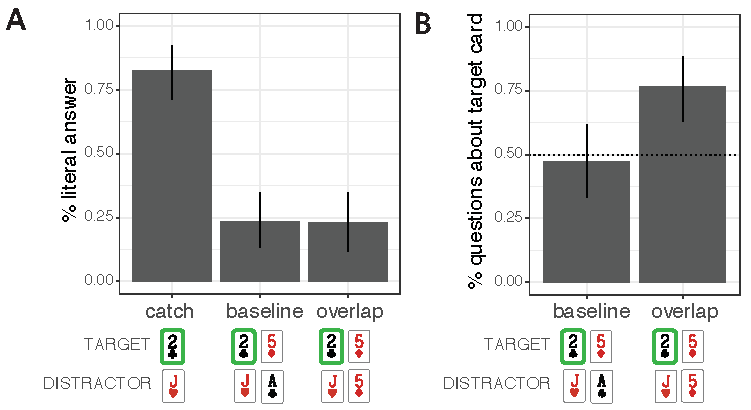
\includegraphics[scale = 1]{Exp2/qualitativeResults.pdf}
\end{center}
\caption{Results for Experiment 2. (A) Answerers are more likely to go beyond the literal question and reveal additional cards in the baseline and overlap conditions. (B) Questioners are more likely to ask about the non-overlapping card relative to baseline. Dotted line is chance, and error bars are bootstrapped 95\% CIs.}
%\vspace{-1cm}
\label{fig:exp2results}
\end{figure*}

The primary computational consequences of introducing a hierarchical goal space emerge from the pragmatic answerer $A_2$. 
Upon hearing a question, $A_2$ must jointly infer the ultimate goal along with the current subgoal.
First, we assume that a questioner acting under an ordered pair $g_{ij} = (g_i, g_i^{(j)})$ attempts to gain information towards both goals:
$$P_{Q}(q | g_{ij}) = \prod_{g\in \{g_i, g_i^{(j)}\}} P(q | g)$$
In other words, a question is preferred if it is both good for the current subgoal and the ultimate goal.
% of finding the entire privately assigned combo $i$.
Combining this assumption about the questioner $Q_1$ with the dependence between subgoal and ultimate goal, $A_2$'s goal inference factors as:
$$\begin{array}{rcl}
P(g_{ij} | q) & \propto & P(q | g_{ij})P(g_{ij}) \\
 & = & P(q | g_i)P(g_i) \cdot P(q | g_i^{(j)}) P(g_i^{(j)} | g_i)
 \end{array}$$
Given a posterior over the goal tuple $g_{ij}$, we then assume the answerer attempts to be informative with respect to both goals in the tuple: 
$$U_{A_2}(a; q, w) = \sum_{g_{ij} \in \mathcal{G}} P(g_{ij}|q) \sum_{g\in \{g_i, g_i^{(j)}\}}\widehat{P^g_I}(w|\,a)$$
While this presentation was written in terms of ordered pairs, it straightforwardly extends to deeper goal hierarchies represented as $n$-tuples. 
The simpler goal spaces considered earlier in the paper are special cases of this more general formulation taking goal tuples to be singletons.

Given this generalization of the model to more structured goal spaces, we can derive predictions for Experiment 2. 
The world space $\mathcal{W}$ consisted of all assignments of cards to locations.
Questions in the question space $\mathcal{Q}$ were of the same form as in Experiment 1 (``Where is the X?''), but because X was always constrained to be a unique card, issues of saliency do not arise. 
Finally, the answer space $\mathcal{A}$ consisted of any combination of one or two card locations, which evaluate to true in worlds where the card or cards are in fact at location that was mentioned, and false otherwise.


\subsubsection{Answerer results}

Although the different conditions of the experiment were primarily designed as a stronger qualitative test of the questioner model, it also provides another opportunity to test the answerer models. 
To begin, consider the simple catch trials, where each goal contained only one card.
Here, both $A_1$ and $A_2$ make the same prediction: that participants will reveal the single card that was asked about with high probability and, with lower probability, they may be ``overinformative'' by revealing both the card that was asked about along with some other card.
Indeed, we found that 83\% of participants responded literally with the exact card asked about, while the remaining 17\% gave overinformative responses (Fig. \ref{fig:exp2results}A).
The precise probability the models put on such overinformative responses depends on the optimality parameter $\alpha$ and a cost parameter penalizing longer answers; at a cost penalty of $1$, the empirical response distribution is obtained with moderate values of $\alpha=3$ for $A_2$ and $\alpha = 3.5$ for $A_1$.

In the \emph{baseline} and \emph{overlapping} conditions, however, $A_1$ and $A_2$ make diverging predictions. 
$A_1$ treats these conditions the same as the catch trial, since it attempts to be directly informative with respect to the goal inherent in the question, and all questions are about a single card.
$A_2$, on the other hand, goes beyond the literal question to infer that the questioner asked about just one subgoal of one of the ultimate goals.
When asked about a card that appears in one goal combo but not the other, $A_2$ infers with high probability which of the two ultimate goals is most likely the hidden goal. 
It is thus much more likely to respond with \emph{both cards} than about only the single card that was asked about (or any other combination of cards). 
We found that only 23\% of participants gave literal answers in each of these conditions, which is significantly different than the proportion (83\%) in catch trials, $\chi^2(1) = 35, p < 0.001$, Fig. \ref{fig:exp2results}A.
The empirical response distributions for these conditions are thus consistent with the predictions of $A_2$ and strongly falsify $A_1$.

\subsubsection{Questioner results}

Next, we turn to questioner behavior, the primary focus of Experiment 2.
The $Q_1$ and $Q_2$ models make qualitatively different predictions about which questions participants chose in the \emph{overlap} and \emph{baseline} conditions.
$Q_1$ predicts no difference in behavior across these two conditions.
Because it reasons that $A_1$ will always provide a literal or (indiscriminately) overinformative response, as we saw in the previous section, then asking about either card is equally useful for completing the target combo.

The pragmatic questioner $Q_2$, on the other hand, recognizes that certain questions may provide better signals about the ultimate goal than others.
In particular, for the \emph{overlap} condition, $Q_2$ reasons that if they asked about the card appearing in both combos, $A_2$ would not be able to infer which of the two combos is their ultimate goal.
If they instead asked about the unique card, however, $A_2$ would infer their true goal with high probability and subsequently be more likely to reveal the needed information.
Thus, $Q_2$ predicts that participants will prefer to ask about the unique card.
The \emph{baseline} condition serves as a control where both cards are unique, hence both questioner models predict no preference over the two cards.

We found that 77\% of participants asked about the unique card in the overlap condition, which is significantly different from the null probability of 50\% predicted by $Q_1$, $\chi^2(1) = 11.3, p < 0.001$. 
Meanwhile, the proportion of participants (48\%) who asked about the card in the same position in baseline trials did not differ from chance: the Bayes Factor for binomial proportions  \cite{morey2016philosophy, morey2015package} shows weak evidence in favor of the null, $BF = 0.37$, Fig. \ref{fig:exp2results}B. 
This qualitative pattern of responses is consistent with the predictions of $Q_2$ but cannot be explained by $Q_1$.

It was possible, however, that this pattern was driven by participants who had already seen their partner ask about the unique card on a previous trial and were copying their behavior. 
To address this concern, we examined these response patterns for the subset of participants who were assigned the role of the questioner on the first half of trials and thus had no opportunity to learn from their partner: 18 of these 21 participants (87\%) asked about the unique card, which remained significantly different from chance: $\chi^2(1) = 9.3, p = 0.002$.

\subsection{Discussion}

Experiment 2 was motivated by two primary aims: to provide a stronger evaluation for the questioner models, and to demonstrate how our core framework generalizes to more structured spaces of goals.
To meet these challenges, we designed a Hidden Goal task where questioners were privately assigned a set of \emph{multiple} objects to find, inducing a hierarchy of subgoals.
By manipulating whether objects overlapped or differed across sets in the space of possible goals, we constructed scenarios where our different models made sharply different predictions. 

We found that answerers reasoned beyond the literal subgoal prompted by the question to respond helpfully to the inferred ultimate goal in the hierarchy.
Questioners, in turn, chose to ask about the objects that would most clearly signal their ultimate goal to their partner, even though these different questions would have equal expected information gain under traditional models. 

The minimal goal hierarchy studied in Experiment 2 is a key first step toward formally addressing more structured spaces of goals in cognitive models of question asking and answering. 
However, handling more complex goal structures will require composing our core computational framework with additional mechanisms.
In particular, we relied on the simplifying assumption of different subgoals being \emph{conditionally independent} given their parent in the hierarchy. 
This assumption justified the representation of subgoals as ordered pairs with their parent, as well as the decomposition of the utility such that each subgoal equally contributes to the ultimate goal. 

This assumption is clearly violated in certain real-world cases.
For example, the overarching goal of making coffee decomposes into subgoals of turning on the faucet, boiling water, grinding beans, and so on \cite{jackendoff2007language}. 
These subgoals unfold in time, introducing sequential dependencies.
If we are trying to make coffee in an unfamiliar kitchen, certain questions may only be useful once earlier subgoals have been satisfied, leading to more or less optimal sequences of questions.
Conversely, answerers may take advantage of schematic knowledge of this sequential structure to anticipate subsequent subgoals: if a questioner asks ``Where do you keep your coffee beans?'', they are likely earlier in the process than if they asked ``Do you have a mug?'' 

Deciding how to ask and answer questions in the presence of such sequential dependences in the goal space likely requires a \emph{planning} mechanism over a persistent state.
Planning may also be necessary for integrating the pragmatics of question asking and answering into longer dialogue sequences, as it has been for other domains \cite<e.g.>{bramley2015conservative}.
While introducing such a planning mechanism into our model is outside the scope of this paper\footnote{The optimality of asking questions based on global planning policies, compared to locally `greedy' policies, is not yet well-understood even in the non-social case of querying an oracle, though see \cite{nelson_meder_jones_2018} for recent theoretical progress.}, our final experiment aims to set a foundation for future work by (1) introducing a notion of persistent state into the model and (2) investigating several pragmatic phenomena that emerge from iterating our model forward in time in a step-wise manner.
%In the next section, we set the foundation for future work on more extended dialogue by investigating certain features of multi-round dialogue that do not require planning.

\section{Experiment 3: Extended dialogue}

In our computational framework, an answerer updates their beliefs about the questioner's goals after hearing a question, and a questioner updates their beliefs about the world state after hearing an answer. 
In principle, this step can be repeated multiple times until the questioner's goal is resolved, allowing for an extended sequence of questions and answers: the questioner's posterior over worlds after hearing an answer to their first question becomes the prior for selecting their second, and so on.

In Experiment 3, we developed a final task in the Hidden Goal paradigm to investigate how the pragmatics of asking and answering questions unfolded over multiple exchanges.
This task was designed with several desiderata in mind.
First, we needed a larger and more natural space of goals that weren't always possible to satisfy in a single round.
This would allow us to test our models' predictions about how the answer to one question may influence the choice of a subsequent question, or how the answerer's beliefs about the questioner's goal may shift after hearing additional questions.
Second, although $A_2$'s internal goal inference mechanism was implicit in the success of our model predictions in Experiments 1 and 2, we sought explicit validation of this model component by directly eliciting answerers' beliefs about the questioner's goal.

\begin{figure*}[tbh!]
\begin{center}
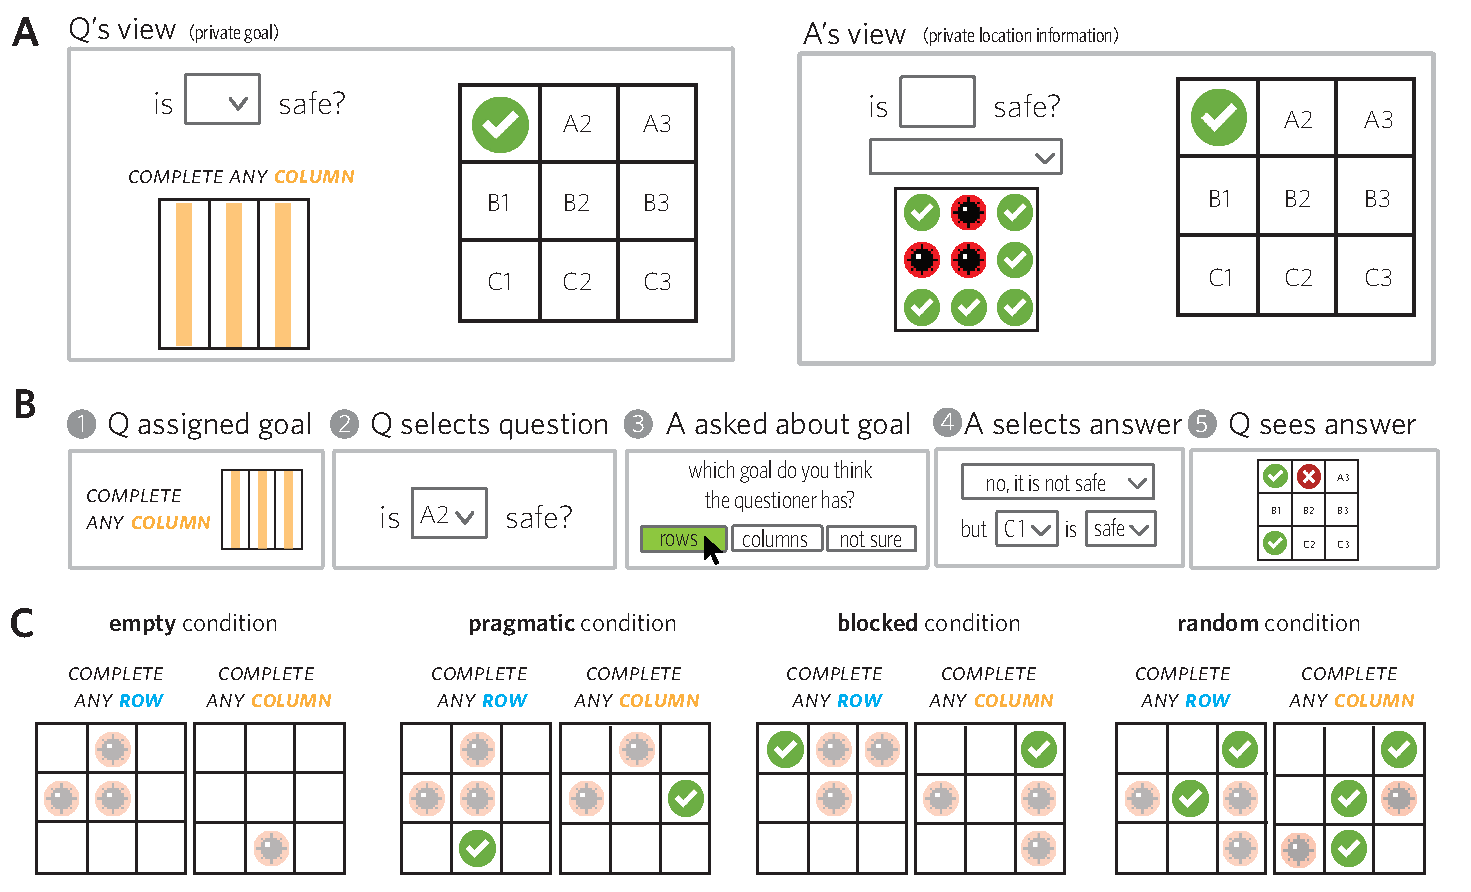
\includegraphics[scale = .7]{Exp3/spatialDemo.pdf}
\end{center}
\caption{(A) Task design and procedure for Experiment 3. Answerers are shown a private map with bomb locations, while questioners are assigned a private goal. Both participants see a common board over which extended dialogues can take place. (B) Examples of initial board states in different conditions.}
%\vspace{-1cm}
\label{fig:exp3task}
\end{figure*}

The \emph{Don't Explode} task is a cooperative communication game inspired by Battleship and Minesweeper (see Fig. \ref{fig:exp3task}). 
Participants are presented with a shared $3 \times 3$ grid and told that some tiles are safe but others contain bombs.
One player---the questioner---is privately assigned a particular goal pattern they must complete by revealing tiles.
The other player---the answerer---is given a map showing where the bombs are.
As in our previous experiments in this paradigm, the answerer has uncertainty about the questioner's goal, and the questioner has uncertainty about the map.
To succeed, then, the questioner must ask questions (e.g. \emph{Is tile X safe?}) and the answerer choose what information to reveal in response.

\subsection{Methods}

\subsubsection{Participants}

We recruited 124 participants from Amazon Mechanical Turk, 21 of whom were excluded for disconnecting before the end of the task. 
This left 104 participants in our final sample. 
All participants were self-reported native English speakers.

\subsubsection{Stimuli}

Each trial was defined by three stimulus choices: (1) a choice of goal, (2) an underlying `map' assigning bombs to locations, and (3) an `initial state' indicating which tiles were shown as safe to both players at the outset of the trial.
By manipulating the state of the initial grid, we generated a large number of items where our models make different predictions. 

Goals were sampled from a space of two ultimate objectives: complete any \emph{row} or complete any \emph{column} (see Fig. \ref{fig:exp3task}A).
Because these goals are logical disjunctions, they could be satisfied in as many ways as there are rows or columns, inducing a hierarchical goal space with each row/column as a possible subgoal the questioner could pursue.
This goal space was intended to be intuitive for participants, given its resemblance to the win conditions of well-known games like Tic-Tac-Toe or Connect Four.

Underlying bomb maps were rejection sampled from the space of all $2^9$ assignments of bombs to locations, subject to the constraint that it was possible to win given either goal. 
We included this constraint so that the arrangement of bombs did not give the answerer any cues to the questioner's goal.
Finally, the initial state of the shared board was chosen from four different conditions to create a variety of different scenarios (see Fig. \ref{fig:exp3task}B for examples).
Cells in the shared board were labeled with coordinates (A1, A2, $\dots$ ) for easy reference.
\begin{itemize}
\item In the \emph{empty} condition, no tiles were included in the initial state%, such that a single question could provide no information to the answerer about the goal.
\item In the \emph{pragmatic} condition, a single tile was included in the initial state. This tile was chosen from a completely safe row or column, depending on the goal.%, such that asking another question in that row or column would provide a clear signal of the goal and allow the answerer to complete the goal after a single question.
\item The \emph{blocked} condition was similar to the pragmatic condition, except a bomb was placed in the row or column partially completed by the initially revealed cell. %This set the grounds for a scenario where questioners may have to adjust their subgoal upon hearing a response.
\item The \emph{random} condition randomly sampled a subset of safe tiles from the map, under the constraint that they did not fully complete a row or column. 
\end{itemize}

\subsubsection{Procedure}

The task procedure was adapted from that of Experiments 1 and 2 to support extended exchanges. 
First, questioners were shown their assigned goal and selected a cell label from a dropdown menu to ask a question of the form ``Is X safe?''. 
Answerers selected a yes/no answer to this question and were presented with the option to either send more information or to continue with only this yes/no answer.
If they chose to send more information, we showed dropdown menus with all possible cells, allowing for responses like ``no, X is not safe, but Y is.''
Finally, this answer was shown to the questioner.
If the new information fulfilled the goal, participants advanced to the next trial.
If the goal was not fulfilled, the questioner was prompted to ask another question, and the cycle repeated.
Participants received a bonus on each trial related to the number of exchanges taken before completing the goal: one cent was subtracted from a total of \$0.05 for each additional question, down to a minimum of \$0.00.

We elicited the answerer's beliefs about the hidden goal after they saw the questioner's message but before they made their response.
Three response options (``rows,'' ``columns,'' or ``not sure'') were provided to the prompt ``Which goal do you think your partner has?'' 
No feedback was provided for this response.
For the other responses, answerers were prevented from sending blatantly false information (e.g. saying there was a bomb when there was no bomb), and questioners were prevented from asking about tiles that had already been revealed.

Participants alternated between the roles of questioner and answerer for a sequence of 20 trials. 
To acquaint participants how the task worked, all trial sequences began with two practice trials, followed by four random trials.
Practice trials were constructed by including two of the three cells of a goal-relevant column or row in the initial state. 
It should have been clear from a basic understanding of the instructions that the questioner needed to ask about the third cell and the answerer ought to reveal it. 
After these initial six trials, we constructed a scrambled sequence where each condition appeared once in each role and these critical trials were interspersed with more random trials.
As in Experiment 2, participants were paired with an artificial agent playing the opposite role. 
This agent responded deterministically according to the output of our $Q_2$ and $A_2$ models. 

\subsection{Results}

\begin{figure*}[tbh!]
\begin{center}
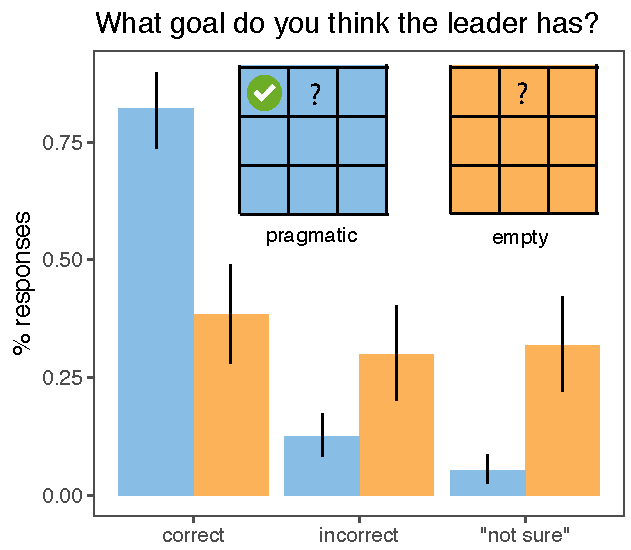
\includegraphics[scale = .7]{Exp3/spatialGoalInference_final.pdf}
\end{center}
\caption{Posterior predictives for each model, which indicate good overall fit (excluding $A_0$ and $Q_0$). Blue dots on $Q$ plots indicate overlapping condition.}
%\vspace{-1cm}
\label{fig:exp3goalinference}
\end{figure*}

\subsubsection{Goal inference results}

The core mechanism driving pragmatic behavior in our models is the goal inference performed by the pragmatic answerer $A_2$, conditioned on the question. 
While the success of $A_2$ in predicting the results of Experiments 1 and 2 provided indirect evidence for this mechanism, the goal belief elicitation step included in the design Experiment 3 provides the opportunity for a more direct test of this mechanism.
How accurately can answerers recover the questioner's true hidden goal from their question utterance?



\subsubsection{Answerer model comparison}

\subsubsection{Questioner model comparison}

\begin{figure*}[tbh!]
\begin{center}
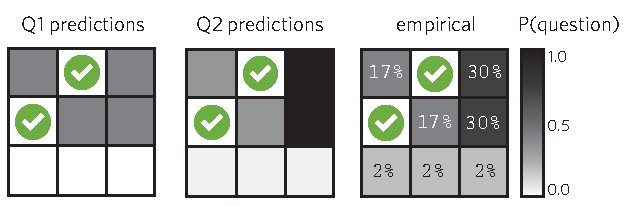
\includegraphics[scale = .7]{Exp3/spatialQualitativeQuestioner.pdf}
\end{center}
\caption{Posterior predictives for each model, which indicate good overall fit (excluding $A_0$ and $Q_0$). Blue dots on $Q$ plots indicate overlapping condition.}
%\vspace{-1cm}
\label{fig:exp1predictives}
\end{figure*}

\subsection{Discussion}

\cite<e.g>{khani2018planning,young2013pomdp,gao2019neural}

\section{General discussion}
\label{sec:gd}

%\todo[inline]{Might split this into subsections?}
% \subsection{Summary of what we did}

Asking questions is one of our most efficient and reliable means of learning about the world. Yet we do not often pose these questions to an impartial oracle; we ask other agents, in dialogue. In this paper, we jointly consider the decision problem faced by each agent. Questioners must plan over the possible answers they are likely to receive from their partner and seek to maximize the future reduction in their own uncertainty. Answerers, in turn, seek to informatively and relevantly address the underlying questioner goals most likely to have generated the question. 

%\todo[inline]{Refactor next paragraph to separate out stuff that's included in the model from external stuff}
We provided several lines of evidence supporting this theory---formalized in our $A_2$ and $Q_2$ models---over purely informative answerers and asocial oracle questioners. In a series of answerer simulations, we showed that only $A_2$ could qualitatively account for classic answerer-sensitivity effects from \citeA{Clark79_IndirectSpeechActs}: answers depend critically upon the question utterance, the context in which a question is asked, and the relationship between the questioner's underlying goal and their question. We then found strong evidence for $A_2$ and $Q_2$ using question and answer data jointly collected from a real-time, multi-player dialogue experiment, which was further bolstered by enriching our literal question semantics with measured saliency priors. %as well as strong quantitative evidence from a rigorous model comparison on trial-by-trial data. By  in this experiment, we also observed systematic use of indirect questions, as predicted by $Q_1$ and $Q_2$. However, only $Q_2$, who relies on higher-order pragmatic reasoning about what goals an answerer would infer from their question utterance, could account for the critical overlapping condition. 
%Finally, enriching the semantics of ``Where is \emph{the}\dots?'' questions to use more realistic saliency priors both eliminated a potential confound and also significantly improved our quantitative fit. %, questioners relied on higher-order pragmatic reasoning about what inferences an answerer would make about their own underlying goals when deciding what question to ask, but a Bayesian model comparison showed that the simpler explicit model is sufficient to explain the vast majority of our data.

%In the case of our Experiment 1 hierarchy, there exists a simple, heuristic strategy that produces the same pattern of responses as our model without requiring any social inference. Suppose questioners saw their goal on a given trial and ruled out labels that do not apply (e.g. a `cat' is neither a `dalmatian' nor a `dog'), then picked the most specific of the remaining labels (`pet' picks out a smaller set of objects than `animal'). Whether through use of this heuristic strategy or pragmatic inference (as our model suggests), questioners strongly converged on a single mapping from goals to question utterances. 

% Note that this behavior also could not be explained by the heuristic strategy raised in the earlier experiments: if questioners just ruled out labels that did not apply (e.g. ``lion''), they would have no mechanism for deciding between the two equally-good parent labels (``pet'' and ``cat'') to pick out their goal. 

A major formal advance of the models considered here is synthesizing current approaches to optimal question asking and answering from AI and linguistics with the recursive social reasoning captured in the Rational Speech Act framework. In addition to introducing pragmatics into the former approaches, this moves RSA models beyond production or interpretation of single utterances (in context) to consider the dynamics of simple dialogs where both listening and speaking---linguistic input and output---must be integrated within the same agent. 

Our computational framework also has implications for the theoretical treatment of question and answer meanings in linguistics and philosophy of language. 
First, while the projection-based question semantics we use as the explicit meaning of questions is equivalent to classic partition-based proposals \cite<e.g.>{GroenendijkStokhof84_SemanticsOfQuestions}, %the meaning of the question can technically be described as its set of possible ``answers,'' i.e. the set of states in the image of its projection map, 
our \emph{answerer} agent chooses from an independent set of declarative utterances $\mathcal{A}$, not from any set of cells constrained by the question. 
This critical dissociation of question meanings, which are informative about \emph{goals} or QUDs, and answer meanings, which are informative about the state of the \emph{world}, is conceptually similar to recent proposals for an \emph{inquisitive semantics} specified in formal logic \cite{ciardelli2013inquisitive, roelofsen2013algebraic}.
The precise relationship between fundamental notions of meaning in inquisitive semantics and meanings in our framework requires further exploration. 
Still, we conjecture that our further dissociation between underlying semantic meaning and recursive probabilistic mechanisms for goal inference and signaling \emph{given} these meanings may be key to grounding pragmatic question and answer behavior in basic social cognitive mechanisms.

\todo[inline]{Need to tune this up; maybe read inquisitive semantics stuff more closely?}
Second, our dissociation of question meanings and goals or QUDs raises the interesting possibility that the set of utterable questions is effectively a \emph{subset} of the possible goals one might have: there may not exist an easy-to-express question utterance for every underlying goal an agent may need to address, thus the need for pragmatics.
%The formulation of these utilities provides a useful connection to current game-theoretic and decision-theoretic models \cite{VogelBodoiaPottsJurafsky13_GricePOMDP, VanRooy03_QuestioningDecisionProblems}, which also emphasize the importance of goals and speaker beliefs in communication.
%Here, we focused specifically on two sub-cases that are of particular interest for psychological science: (1) selecting a question in the absence of any input, and (2) selecting a declarative statement in response to a question. 
%In principle this framework allows a dialogue agent to update their beliefs after hearing any type of utterance, then to select any type of utterance in response. 

%The former requires replacing the immediate motive to convey true information with the more distant motive to provoke useful information from one's interlocutor. The latter requires sophisticated inference about the underlying interests of the questioner instead of simply relying upon the literal question semantics. 

% Questioner behavior, however, appeared to be more sensitive to the experimental set-up. In a single-player pilot version of Exp.~1, for example, we did not emphasize certain aspects of the game in the instructions, such as the fact that the answerer knows about the restricted answer set. Our data in this pilot experiment appeared to contain a mixture of explicit and pragmatic answerers and questioners (though other confounds were present in this version). We found the interactive, multi-player version of the task, used in this paper to be more robust to these minor variations. 

%\subsection{Limitations of the model}

%We emphasize that all our models are situated firmly at the computational level \cite{Marr10_Vision} -- these models formalize hypotheses about the problem being solved by questioners and answerers in dialogue, and they make quantitative predictions about expected behavior under different assumptions. However, we do not propose that people are actively running a recursive probability calculation online every time they ask a question; further work is needed at the algorithmic and mechanistic levels to understand exactly what cognitive and neural processes give rise to the computations we predict, especially when it comes to integrating information across discourse contexts. 

%While these results provide strong evidence for our claim that question-asking and answering is grounded in sophisticated social reasoning, it is worth more closely examining some choices we made in formulating our Rational Speech Act model. For example, as in previous studies using RSA, we assume that the recursive reasoning process giving rise to pragmatic interpretations grounds out in a base case of literal semantics. We only consider two levels of recursion above this base case, but we could in principle consider a fixed-point at infinity \cite{Franke13_GameTheoryPragmatics}. Alternatively, social reasoning could be grounded not in iterated reasoning but in a joint project or shared intention established by other means \cite{Clark96_UsingLanguage, TomaselloCarpenter___Moll05_IntentionsCulturalCognition}. While we suspect the question-answer domain is not particularly informative for distinguishing between these formulations, we note that additional levels of reasoning tend not to qualitatively change RSA predictions and that our model contains elements of the latter proposal in its assumption that questioners and answerers share priors, sets of alternatives, and semantic meanings in common ground \cite<see>[for further discussion]{LassiterGoodman15_AdjectivalVagueness} 

Our model also complements recent work enriching active learning paradigms to allow rich natural-language questions as queries \cite{RotheEtAl16_NaturalLanguageQuestions, CohenLake16_20Q}. The expected information gain (EIG) measure used to choose new queries in these studies is closely related to our questioner formulation. Our most critical innovation to this line of work is embedding active learning in a social, communicative context \cite<see also>{ShaftoGoodmanFrank12_LearningFromOthers, ShaftoGoodmanGriffiths14_Pedagogical}. Instead of computing expected information gain across \emph{all possible} answers, our questioner models take the expected value over a cooperative \emph{dialogue partner} who seeks to be informative and relevant, often going beyond the literal question meaning. This allows questioners to effectively ask indirect questions and is especially important in real-world contexts where there is legitimate uncertainty over the questioner's goals; in a twenty-questions game, the questioner always has the goal of guessing the target object, but in a classroom context, the goal motivating a student's question may not be as obvious. 
%This allows many classic active learning tasks in cognitive psychology can be modeled as special cases of our \emph{explicit} questioner model. There are two main ways that our framework generalizes Bayesian models of active learning (e.g. XXX): first, it allows for the full range of questions expressible under our natural language semantics rather than restricting the learner to narrow yes/no questions like ``Is this an example of category A?'' Second, because the answerer is a social agent capable of reasoning about the questioner's underlying goals, the questioner could in principle rely on the cooperativity principle to ask additionally informative questions. 

How do our assumptions scale up to less constrained interactions? We suspect that the simple, discrete sets of QUDs used in our models above will need to be generalized to continuous spaces and broader mixtures of discourse topics \cite{BleiNgJordan03_LDA, GriffithsSteyversTenenbaum07_Topics}. The computational challenges associated with such complex QUD spaces may contribute to the difficulties young children face in answering broad, sentence-focus questions like ``what's happening?'' \cite{SalomoLievenTomasello13_ChildrenAnsweringQuestions}. To generalize beyond the hand-picked sets of alternative questions and answers used in our models above, we may need to consider conditional frequencies from past interactions or simple deletions and edits from the given question \cite<e.g.>{GibsonBergenPiantadosi13_RationalIntegrationNoisy}. To generalize to dialogues lasting longer than a single exchange, we must specify the way in which the contributions of questioner and answerer affect the \emph{context} in which later utterances operate, and the longer-term planning needed for agents to reason effectively about such interactions.

%Finally, although our Bayesian model comparison strongly favored the lower-level questioner model, indicating that the burden of pragmatic reasoning lies primarily on the answerer, it is still unclear under which circumstances questioners engage in an additional level of recursion. In a critical condition designed to test between the models, participants  displayed evidence of this additional level of reasoning, but the difficulty of constructing such a case suggests that such circumstances may be rare. 
%\todo[inline]{Not sure they're actually that rare... Might just be accessibility bias or difficulty of construction in our experimental paradigm?}
%It will ultimately be important to explore the mixture of explicit- and pragmatic-questioning across an even larger range of situations: these issues may be a product of our artificial game paradigm, or they may be reflective of real tendencies in language use, raising novel questions about audience design in question-answer behavior. 

%\subsection{Extensions and comparisons to previous models}

%The probabilistic model we have presented bears some resemblance to recent decision theoretic \cite{VogelBodoiaPottsJurafsky13_GricePOMDP} and game theoretic \cite{Franke13_GameTheoryPragmatics} models of pragmatic reasoning in language use. In particular, all these approaches emphasize \emph{inference} about a partner's underlying mental state. In this respect, these theories contrast with the interactive alignment model \cite{PickeringGarrod04_BBS_Dialogue} and competing dynamical systems models of dialogue \cite<e.g.>{FusaroliTylen15_Synergy}, where coordination occurs through a low-level process of priming and adjusting to a partner's syntactic, lexical, and phonological choices. 


%Second, note that our model assumed basic prosociality on the part of the answerer: the questioner expects the answerer to be helpful even though there is often no direct reward for stopping to help. Some of the most intriguing question-answering scenarios, however, flout this expectation. In politics or court of law, for instance, it is sometimes in the answerer's best interest to be minimally informative while still  addressing the explicit semantics of the question. To understand answers in these cases, or to identify when an answerer is being uncooperative, we might flip the answerer's utility to \emph{minimize} the reduction in questioner uncertainty or ``lift'' this variable such that the questioner is uncertain and must infer whether the answerer is prosocial. 

%Next, consider how we could account for questions asked by parents or educators \cite{MaradlouGinzburg14_SemDial, Gall70_QuestionsInTeaching}.: a math instructor asking a question like ``what is $2+2$?'' already knows the answer, so what utility could there be in asking? Instead of trying to reduce their own uncertainty over the result of the math problem, perhaps the teacher is instead trying to reduce their uncertainty over the child's knowledge state. In all the simulations and experiments reported above, we assumed that questioner and answerer share a fixed knowledge structure in common ground (e.g. of the hierarchical relationship between dalmatians, dogs, and animals). If we relax this assumption and allow uncertainty over the answerer's knowledge, then the questioner might ask targeted questions to learn exactly what the answerer believes. 

%As a final example of potential extensions of our model, we return to the case of politeness, which often motivates indirect questions like ``Do you know where I can find a restroom?'' The same considerations may influence answerer behavior as well. We often use more words than necessary to avoid seeming curt. For instance, literal `yes' answers are often something like `yes, I do' or `no, but good luck!' One way to think about this is that the questioner has some uncertainty over the answerer's relative balance between utterance cost and helpfulness, and questioners will jointly infer this. A pragmatic answerer reasoning about this kind of questioner, then, will choose answers not just to reduce the questioner's uncertainty over the QUD but also to signal that they value helping. 

%While the artificiality of our question-answer game may distance the behavior of participants from the natural use of language, there are also some benefits to this design. In particular, it is easy in this setting to control the exact space of questions, goals, and answers. While the restrictions on question space may seem peculiar, it is directly motivated by conversational scenarios in everyday usage which feature restrictions on the set of things one can ask about, due to politeness, salience, time cost, and other factors. 

Humans are experts at inferring the intentions of other agents from their actions \cite{TomaselloCarpenter___Moll05_IntentionsCulturalCognition, BakerSaxeTenenbaum09_ActionUnderstandingInversePlanning}. Given simple motion cues, for example, we are able to reliably discern high-level goals such as chasing, fighting, courting, or playing \cite{BarrettToddMillerBlythe05_IntentionFromMotionCues, HeiderSimmel44_Animacy}. A long tradition in psycholinguistics has shown that this expertise extends to speech acts.  Behind every question lies a goal or intention. This could be an intention to obtain an explicit piece of information (``Where can I get a newspaper?''), signal some common ground (``Did you see the game last night?''), test the answerer's knowledge (``If I add these numbers together, what do I get?''), politely request the audience to take some action (``Could you pass the salt?''), or just to make open-ended small talk (``How was your weekend?''). These wildly different intentions seem to warrant different kinds of answers. %, even if the explicit question is expressed using the same words
%\todo[inline]{Reformulate this last sentence so that it doesn't sound like we've already accomplished this; make clear that this is something for the future, but that the framework is really exciting because it?s so clear about where one would start fiddling with it}
By formalizing the recursive utilities of questioner and answerer agents and the computational principles by which agents infer each other's intentions from verbal behavior, our theoretical framework provides a foundation for re-situating dialogue in its social context and capturing the full richness of dialogue behavior.

\section{\bf Acknowledgments}
\small
\noindent We thank Leon Bergen, Judith Degen, Arianna Yuan, MH Tessler, and Judith Fan for thoughtful conversations and comments. This work was supported by ONR grants N00014-13-1-0788 and N00014-13-10341. RXDH was supported by the Stanford Graduate Fellowship and the National Science Foundation Graduate Research Fellowship under Grant No. DGE-114747.

\bibliography{qa}
\bibliographystyle{apacite}


\begin{table*}[t!]
\centering
\begin{tabular}{ p{1.5cm} | r | r | r | r |||||| r | r | r | r |}
& \multicolumn{4}{c||||||}{Questioners} & \multicolumn{4}{c}{Answerers} \\
&             animal &     place &     plant &  artifact &            animal &     place &     plant &  artifact \\
\hline
animal &   1.00 &  0.91 & 0.94 & 0.94 & 1.00 & 0.78 & 0.92 &  0.97 \\
\hline
place &    0.91 &  1.00 & 0.96 & 0.95 & 0.78 & 1.00 &  0.78 & 0.78 \\
\hline
plant &    0.94 & 0.96 & 1.00 & 0.97 & 0.92  & 0.78 &  1.00 & 0.91\\
\hline
artifact & 0.94 & 0.95 & 0.97 & 1.00 & 0.97 & 0.78 &  0.91 & 1.00\\
\end{tabular}
\\[1.5pt]
\caption{Appendix: Inter-domain correlations on corresponding response rates} 
\label{table:experiment4correlations}
\end{table*}

%\section{Appendix}
%
%\subsection{Groenendijk and Stokhof (1984)}
%%\begin{figure*}[t!]
%%\begin{center}
%%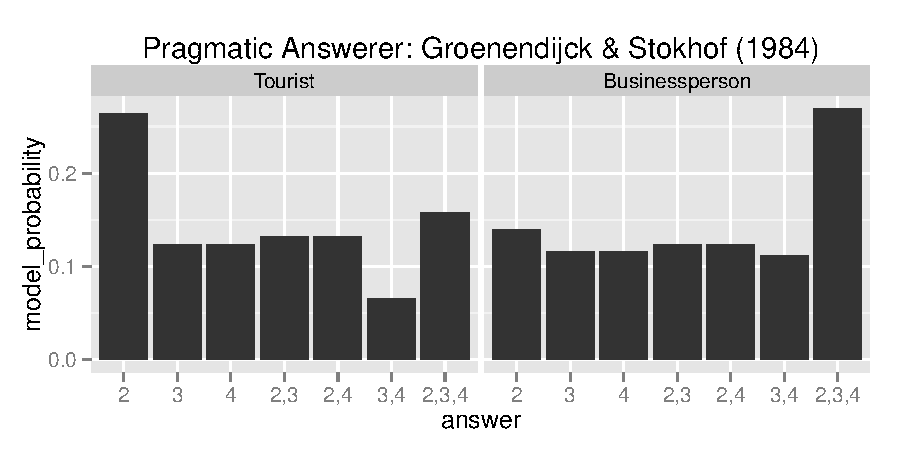
\includegraphics[scale = 1]{groenendijckPlot.pdf}
%%\end{center}
%%\vspace{-.25cm}
%%\caption{Results for our computational experiments implementing the Groenendijck \& Stokhof (1984) \emph{mention-some} problem.}
%%\label{fig:cafeExperimentResults}
%%\end{figure*}
%
%%Here, we consider the classic puzzle of \emph{mention-some} and \emph{mention-all} readings of wh-questions  \cite{GroenendijkStokhof84_SemanticsOfQuestions}. 
%Some \emph{wh-}questions, like ``Who is coming to dinner tonight?'' are intended to elicit an \emph{exhaustive} list of the entities that are answers. For ostensibly similar questions, like ``Where can I find a bathroom in this building?'', a mention of a single location would be sufficient. Many recent theoretical explanations of this phenomenon in the linguistics literature appeal to questioner goals \cite<e.g.>{SchulzVanRooij06_ExhaustiveInterpretation, Ginzburg95_ResolvingQuestions}, which is easily formalized in our model as a context-prior. 
%
%We focus on a question like ``Where do they sell Italian newspapers in Amsterdam?'' that can intuitively be ambiguous between these meanings depending on who is asking: if it is a tourist, they probably just want to know the nearest place, but if it is a businessperson trying to build a newspaper distribution network, they likely want the whole list \cite<see>{GroenendijkStokhof84_SemanticsOfQuestions}. The puzzle is  one of disambiguation\footnote{Our modeling framework is compatible with another account where the `mention-some' reading is derived from the exhaustive reading via implicature \cite<e.g.>[Chapter 6]{George11_Dissertation}, but this debate lies outside the scope of this paper}: how can the same question take on different meaning in different contexts? According to our account, this happens via an inference about the questioner's underlying goal. This explanation relies on the same mechanism as the previous section, but shows how the model can operate over more complex world states and arbitrarily large spaces of possible answers.
%
%Our world space $\mathcal{W}$ consists of all possible assignments of properties to a set of four cafes in town. Each cafe has two properties: its distance from the speaker and whether or not it sells Italian newspapers. There are two possible goals (or QUDs) $g \in \mathcal{G}$: $g_{n}$, learning the identity of the \emph{lowest-cost} cafe selling a newspaper, and $g_{a}$, learning the identity of \emph{all} cafes selling a newspaper. Both of these are represented by projections on world states, mapping a list of cafes to the single cafe selling newspapers with the lowest distance -- assuming that additional distance incurs additional cost -- or to the sublist that sell newspapers, respectively. \ndg{why talk about cost, rather than just saying closest?} The space of answers $\mathcal{A}$ is the infinite set containing all conjunctions of locations. \ndg{is that infinite? up to redundancy it's large but finite?} Again, our question space $\mathcal{Q}$ consists of a single question: ``Where can one buy an Italian newspaper?'' \ndg{what literal meaning do we assign to this question?}
%
%For the prior $P(a)$ over answer utterances, we use a geometric distribution, which is common over spaces where probabilities should naturally scale with some count. Let $\ell(a)$ be the number of locations named in the answer (e.g. $\ell(\textrm{`none'})~=~0, \ell(\textrm{`cafe 1'})~=~1$, etc). Then the probability of an answer $a$ is given by:
%
%$$P(a) \propto (1 - p)^{\ell(a)}p$$
%In our computational experiment, we fix $p = 0.8$. 
%This simple distribution has two advantageous properties: 
%\begin{enumerate}[(1)]
%\item the probability mass assigned to a given utterance length -- operationalized as number of conjunctions -- by the geometric distribution is spread evenly across different answers of that length.
%\item we naturally assign longer answers successively lower probability, reflecting their higher cost of utterance. \end{enumerate}
%
%\ndg{i think we can a say a lot less about this prior: just that we assume the cost of an answer is proportional to it's length, hence the prior is proportional to $\exp(length)$...}
%
%
%We model the non-verbal context as affecting the questioner's goal prior $P(g)$: if they are a tourist on the street then there's a high chance that they are interested in buying a single newspaper, and hence knowing the identity of the closest shop that sells Italian newspapers ($P(g_n | c) = 0.99$); if they're a businessperson in a boardroom, then there's a high chance that they are interested in the exhaustive list of all of the Italian newspaper locations ($P(g_a | c) = 0.99$).
%
%%\footnote{Note that this formulation of the problem differs slightly from the one given by \citeA{GroenendijkStokhof84_SemanticsOfQuestions}, although they easily map onto one another. In the original formulation, the \emph{answer} is fixed and the \emph{meaning} of the answer must be inferred to either be mention-some or mention-all. In our formulation, the meaning of each answer is unique and fixed, but the answerer must choose among a set of different possible answers. The same inferential machinery that our questioner uses to reason about which answer utterance the answerer will give could also be used to reason about which \emph{meaning} the answerer intends by their fixed utterance. The only difference is that the questioner would have uncertainty over a set of possible meanings instead of uncertainty over a set of possible answer utterances. We chose the latter because it more closely resembles the other scenarios we are modeling.}
%
%It is unclear where these goals and goal priors may come from in real-world situations: it is likely tied to background knowledge about tourists, newspapers, and the business world, as well as past experience in social situations. While these deeper explanations lie outside the scope of our model, we still have explanatory power in showing how goals interact with other terms, and how the prior differ across scenarios. 
%
% \begin{figure*}[t!]

%\ndg{i didn't re-read this appendix... there seem to be old comments of mine left?}

%\begin{figure*}[t!]
%\begin{center}
%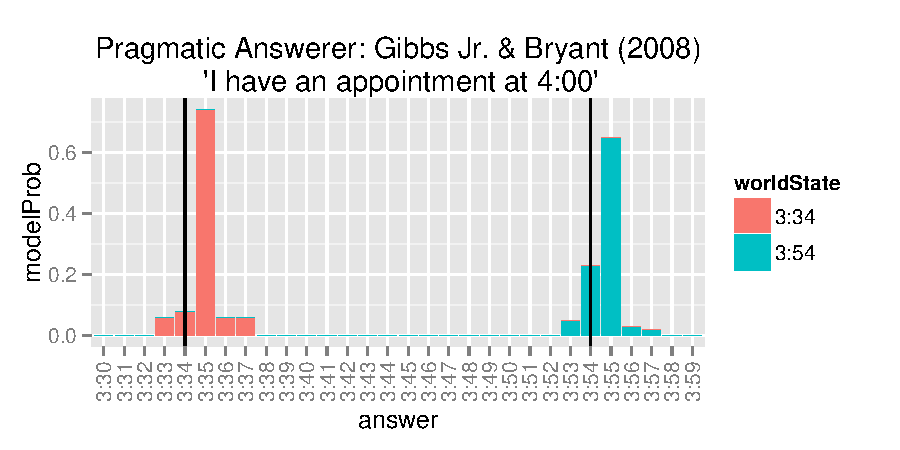
\includegraphics[scale = 1]{timeExpResults.pdf}
%\end{center}
%\vspace{-.25cm}
%\caption{Results for our computational experiments replicating Gibbs Jr. and Bryant (2008). Vertical lines represent the true world state.}
%\label{fig:timeExperimentResults}
%\end{figure*}
%
%\subsubsection{Results}
%
%For concreteness, we set the true world to be the following :
%
%\begin{lstlisting}
%world = {`cafe1' : [3, false],
%         `cafe2' : [1, true],
%         `cafe3' : [3, true],
%         `cafe4' : [3, true]}
%\end{lstlisting}
%meaning that `cafe1' is three blocks away from the speaker and does \emph{not} sell Italian newspapers, `cafe2' is one block away and \emph{does} sell Italian newspapers, and so on. We used \emph{likely-first enumeration} over the answerer model, stopping after 1000 executions of the infinite answer space (longer answers were assigned vanishingly small probability). We find that the highest probability response given the ``tourist'' context is the single location ``cafe2.'' When worlds consistent with this utterance (i.e. where cafe2 truly sells an Italian newspaper) have been projected to the closest location, the actual closest location has high probability, thus informatively fulfilling the contextually more likely goal $g_n$. Note that longer responses are unlikely for two converging reasons: they're less likely under the geometric answer prior and also may mislead the questioner into thinking another location is the closest. 
%
%Given the ``businessperson'' context, however, the highest probability response is the conjunction ``cafe2 and cafe3 and cafe4.'' This is the exhaustive answer, informatively fulfilling the contextually more likely goal $g_a$ of knowing the location of all cafes selling Italian newspapers. Shorter answers are less likely; they are consistent with more possible worlds in the projected space, hence the projection of the true world has lower probability. 
%
%\ndg{it occurs to me that if you ignored the question and just took the goal to be the qud you'd get the same results. maybe we'd like to have a more likely a priori goal that get's dis-preferred after hearing the question? for instance the identity goal could be a priori more likely, but then becomes less plausible after hearing the question about italian papers?}
%
%%The literal and explicit answerers, as in the Clark scenario, do not have the means of making inferences about the questioner's underlying goals. Thus, both models incorrectly predicted that the context would not affect the preferred response. The literal answerer predicted that all combinations of cafes 2, 3, and 4 would be given in proportion to their prior likelihood (with no special preference given to the closest one). The explicit answerer predicted that the exhaustive answer would be preferred in all contexts (as this is literal semantics we encoded for the question). 
%Crucially, the only difference between our model of this scenario and the Clark scenario is the richer representations of multi-dimensional world states, and the larger (unbounded) space of answers. The model itself was unchanged; we only enriched the content of its inputs. The mechanism by which goals were inferred in both cases, however, was the same: a direct function of verbal or non-verbal context. Next, we turn to a case where the world state itself provides a clue to the questioner's goal.
%%%%%
%
%
%\subsection{Gibbs Jr. \& Bryant (2008): Experiment 3}
%
%It has been shown in previous work that speakers typically round their answers to the nearest 5 minute interval when asked `Do you have the time?'', even when they're wearing a digital watch \cite{DerHenstCarlesSperber02_RelevanceTellingTime}.  \citeA{GibbsBryant08_OptimalRelevance} replicated this result, and then performed a follow-up study on analog-watch wearers where they preceded their question by the context ``I have a meeting at 4:00.'' 
%
%They found that the tendency to round times decreased as a function of the time remaining until the stated deadline: the group asked 30-16 minutes before the stated appointment rounded their responses 79\% of the time, while the group asked 14 minutes or closer to the appointment rounded significantly less (62\%). They explained this result by appealing to the questioner's goals: while an approximate time is sufficiently informative with respect to most goals, such as knowing how much time is left before heading to an appointment, a questioner who is running late may need to gauge how quickly they should move, whether they should call and warn about being late, or make other such decisions, in which case a precise time is highly relevant. 
%\begin{table*}[t]
%\centering
%\begin{tabular}{ p{2cm} | r |||||| r }
%&  \% round (Empirical) &  \% round (Model) \\
%\hline
%Early group &  0.79 & 0.77 \\
%\hline
%Late group     &0.62  & 0.60 \\
%\end{tabular}
%\\[1.5pt]
%\caption{Comparison of our model predictions with data from Gibbs Jr. and Bryan (2008). Shows the proportion of rounding in response to ``I have an appointment at 4:00. Do you have the time?'' for two groups: an ``early group'' where the appointment was in 30-15 minutes and a ``late group'' where the appointment was in less than 15 minutes.} 
%\label{table:gibbsJrExp3}
%\end{table*}
%
%To set up this scenario in our model, we take the world space to be the set of possible times, which we limit to a half hour interval (as in the experiment): $\mathcal{W}~=~\{\textrm{3:30}, \textrm{3:31}, \dots, \textrm{3:59}\}$. Unlike in the previous two case studies, where there were only two contrasting goals and two contexts that make each goal more or less likely, we now use a larger, parametrized goal space and a single context stating the time of the appointment that is held fixed across different conditions of the experiment. 
%
%This goal space $\mathcal{G}$ includes the trivial projection $g_0(w) = w$, corresponding to the context-independent goal of learning the true time, in addition to a set of goals parameterized by a threshold time $\tau$, representing the point at which the agent believes they are running late to their appointment (likely based on expectations about travel time, social norms concerning lateness, and other exogenous factors). If the agent has goal $g_\tau$ for a given $\tau$, then for times $t < \tau,$ the agent only cares about the approximate time, rounded to the nearest 5 minute increment, in order to know roughly how much time they have before leaving. For times $t > \tau$, the agent cares about the exact time in order to make the kind of decisions described above. Formally,
%
%\DeclarePairedDelimiter{\floor}{\lfloor}{\rfloor}
%
%$$g_\tau(w) = \left\{
%\begin{array}{rcl}
%w & & w \ge \tau\\
%5\floor{\frac{w}{5} + \frac{1}{2}} & & w < \tau;  \\
%\end{array}
%\right.
%$$
%where $\floor{w}$ returns the \emph{floor} of an integer and all operations are assumed to act on the minutes component of a time $w$. For example, the goal $g_{3:50}$ with the threshold set at $\tau = $3:50 corresponds to a projection function that rounds input worlds earlier than 3:50 and does not round worlds later than 3:50. This would be the case if the agent knew they would need to leave around 3:50 in order to make it to an appointment on time. 
%
%The goal prior $P(g_\tau)$ assigns probability $p=0.25$ to the context-independent goal $g_0$ of wanting to know the exact time. The remaining probability mass is divided across different threshold goals ($\tau \in \{$ 3:31, 3:32, \dots, 3:59 $\}$) according to the following rule: the likelihood of each goal $g_\tau$ is inversely proportional to the distance (in minutes) between the threshold $\tau$ and the given appointment time $c$, reflecting the intuition that the questioner will be more likely to be running late, and therefore in need of the exact time, as it approaches the appointment time:
%
%$$P(g_0) = 0.25$$
%$$P(g_\tau; c) = \frac{0.75}{\sum_{i=1}^{29}i}(30 - |\tau - c|)$$
%
%The set of answers is the set of times that could be given (e.g. 3:30, 3:31, \dots, 4:00), with multiples of 5 preferred:
%$$P(t) = \left\{
%\begin{array}{lcl}
%0.125 & & t \equiv 0 \mod 5 \\
%0.01 & & \textrm{otherwise} \\
%\end{array}
%\right.
%$$ As \citeA{GibbsBryant08_OptimalRelevance} point out, their participants all wore analog watches, hence precise answers have higher cost. In fact, an earlier study in the same paper showed that in the absence of any context, participants wearing analog watches responded with rounded answers 90\% of the time, so this prior is realistic. 
%
%For our answers, we use exact number semantics: the response ``3:35'' evaluates to true in worlds where the time is in fact 3:35, and false otherwise. While we suppressed \emph{a priori} false answers for convenience in other case studies (they would be naturally be assigned vanishingly small probability anyway), note that we cannot do so here: answerers must be allowed to make \emph{a priori} false utterances that get reinterpreted by the listener to be true under the QUD \cite<see>{KaoWuBergenGoodman14_NonliteralNumberWords}. 
%
%%\todo[inline]{return to this in the discussion}
%
% \subsubsection{Results}
% 
%To compare our model's performance against the `early group' and `late group' conditions in \citeA{GibbsBryant08_OptimalRelevance}, we ran two simulations. In both, the context is ``I have an appointment at 4:00.'' In the first, the true world state is between 3:30 and 3:45 (the `early' condition); in the second, the true world state is between 3:45 and 3:59 (the `late' condition). In each condition, we ran our pragmatic answerer model for all true worlds in the appropriate range of times, and report the average probability of responding with a rounded answer. Our results are compared against empirical data from Gibbs Jr. and Bryant \citeyear{GibbsBryant08_OptimalRelevance} in Table \ref{table:gibbsJrExp3}. 
%
%To more closely analyze what is driving our model's performance in these two conditions, we examine the answer behavior for two specific world states: one from the `early group' (3:34) and one from the `late group' (3:54). Answer probabilities for these two conditions are shown in Figure \ref{fig:timeExperimentResults}. We found that our pragmatic answerer model rounds the 3:34 to 3:35 in the `early' condition with probability $p = 0.74$, but rounds 3:54 to 3:55 with lower probability $p = 0.65$ in the `late' condition. 
%
%The goal prior is the key component of the model governing this difference. Note that that (1) \emph{all} states in the pre-image of the rounding projection from the true time $t_0$ are assigned lower probability than the rounded time $g_\tau(t_0)$, due to the influence of goals $g_\tau$ with thresholds $\tau > t_0$ and (2) the true time $t_0$ is assigned relatively higher probability than the other non-rounded times, due to the influence of the pure goal $g_0$ and goals $g_\tau$ with thresholds $\tau < t_0$. This dynamic, paired with the upward-skewed prior on goal priors discussed above, causes the `late' condition to assign a much higher relative probability to the true time, than the `early' condition. The pragmatic answerer thus accurately captures the empirical results both qualitatively and quantitatively. 

%Our literal and explicit answerer models fail to capture these contextual differences, as they do not reason about the space of underlying goals (which justify rounding) and always give the exact time. The literal answerer always gives the exact time because it is the only property of the world, which they are attempting to be informative about without regard to the question. The explicit answerer always gives the exact time because it uses the explicit question meaning, which simply asks for the time.

%\todo[inline]{rdh: Actually, in the experiment the question was ``Do you have the time?'' to which the literal and explicit answers would be ``yes'' or ``no'', right? We don't allow these responses in our model because they're not what we're interested in (i.e. \emph{no one} responded this way), but they are the kinds of answers our literal and explicit answerers would give}

\end{document}  
